% !TEX TS-program = pdflatex
% !TEX encoding = UTF-8 Unicode
% !BIB TS-program = biber
% !BIB program = biber
\documentclass[12pt]{article}
% REFERENCES
\usepackage[backend=biber,style = apa]{biblatex}
\bibliography{finance-honours.bib}
% \addbibresource{sources.bib}
%%% PAGE DIMENSIONS
\usepackage[margin=2.54cm]{geometry}
\usepackage{setspace}
\doublespacing
\geometry{a4paper}
%%% PACKAGES
% \usepackage{caption}
% \usepackage{subcaption}
\usepackage{graphicx} % For better graphics
% Sets graphics paths
\graphicspath{ {/Users/connor/Google Drive/Documents/University/Courses/2020-21/Finance 788/finance-honours/results/plots}{/Users/connor/Google Drive/Documents/University/Courses/2020-21/Finance 788/finance-honours/results/plots/model-performance} }
\usepackage{grffile}
\usepackage{pdfpages} % To insert pdfs into the library
\usepackage{tikz}
\usepackage{wrapfig}
\usepackage{siunitx}
\usepackage{lscape} % Create landscape orientation for tables
\usepackage{longtable}
\usepackage{booktabs} % for much better looking tables
\usepackage{amsmath} % for better maths
\usepackage{paralist} % very flexible & customisable lists (eg. enumerate/itemize, etc.)
\usepackage{verbatim} % adds environment for commenting out blocks of text & for better verbatim
\usepackage{subfig} % make it possible to include more than one captioned figure/table in a single float
\usepackage[framed,numbered]{matlab-prettifier} % enable inserting matlab code.
\usepackage{tikz} % Package for drawing flow diagrams
\usepackage[parfill]{parskip}
%\addtolength{\jot}{1em}
\usepackage{amssymb}
\usepackage{cancel}
\usepackage{color}
\usepackage{listings}
\usepackage{docmute}
\usepackage{indentfirst}
\usepackage{array}
% DECLARATIONS
\DeclareMathOperator*{\argmax}{arg\,max}
\DeclareMathOperator*{\argmin}{arg\,min} % thin space, limits underneath in displays
% STYLE FORMATTING
\usepackage{xcolor}
\definecolor{codegreen}{rgb}{0,0.6,0}
\definecolor{codegray}{rgb}{0.5,0.5,0.5}
\definecolor{codepurple}{rgb}{0.58,0,0.82}
\definecolor{backcolour}{rgb}{0.95,0.95,0.92}
\lstdefinestyle{mystyle}{
    backgroundcolor=\color{backcolour},   
    commentstyle=\color{codegreen},
    keywordstyle=\color{magenta},
    numberstyle=\tiny\color{codegray},
    stringstyle=\color{codepurple},
    basicstyle=\ttfamily\footnotesize,
    breakatwhitespace=false,         
    breaklines=true,                 
    captionpos=b,                    
    keepspaces=true,                 
    numbers=left,                    
    numbersep=5pt,                  
    showspaces=false,                
    showstringspaces=false,
    showtabs=false,                  
    tabsize=2}
\lstset{style=mystyle}
\usepackage{multicol}
\usepackage{float}
%%% FLOW DIAGRAM STYLE
\definecolor{inputlayercolour}{RGB}{88,129,243}
\definecolor{hiddenlayercolour}{RGB}{14,190,183}
\definecolor{outputlayercolour}{RGB}{146,182,255}
\definecolor{inputcolour}{RGB}{155,177,218}
\definecolor{outputcolour}{RGB}{245,164,191}
\usetikzlibrary{shapes.geometric, arrows}
\tikzstyle{hiddenlayer} = [rectangle, rounded corners, minimum width=3cm, minimum height=1cm,text centered, text width = 5cm, draw=black, fill=hiddenlayercolour]
\tikzstyle{inputlayer} = [rectangle, rounded corners, minimum width=3cm, minimum height=1cm, text centered, text width = 5cm, draw=black, fill=inputlayercolour]
\tikzstyle{outputlayer} = [rectangle, rounded corners, minimum width=3cm, minimum height=1cm, text centered, text width = 5cm, draw=black, fill=outputlayercolour]
\tikzstyle{inputs} = [rectangle, rounded corners, minimum width=3cm, minimum height=1cm, text centered, text width = 5cm, draw=black, fill=inputlayercolour]
\tikzstyle{predict} = [trapezium, trapezium left angle=70, trapezium right angle=110, minimum width=3cm, minimum height=1cm, text centered, text width = 5cm, draw=black, fill=outputcolour]
\tikzstyle{arrow} = [thick,->,>=stealth]
%%% HEADERS & FOOTERS
\usepackage{fancyhdr} % This should be set AFTER setting up the page geometry
\setlength{\headheight}{15pt}
\pagestyle{fancy} % options: empty , plain , fancy
\renewcommand{\headrulewidth}{0pt} % customize the layout...
\lhead{University of Auckland}\chead{Finance 788}\rhead{Connor McDowall}
\lfoot{}\cfoot{\thepage}\rfoot{}
%%% SECTION TITLE APPEARANCE
\usepackage{sectsty}
%%% TABLE OF CONTENTS APPEARANCE
\usepackage[nottoc,notlof,notlot]{tocbibind} % Put the bibliography in the ToC
\usepackage[titles,subfigure]{tocloft} % Alter the style of the Table of Contents
\renewcommand{\cftsecfont}{\rmfamily\mdseries\upshape}
\renewcommand{\cftsecpagefont}{\rmfamily\mdseries\upshape} % No bold!
%%% HYPERLINKING
\usepackage{hyperref}
%%% DOCUMENT
\begin{document}
%%% NEW COMMANDS
\newcommand{\listequationsname}{List of Equations}
\newlistof{myequations}{equ}{\listequationsname}
\newcommand{\myequations}[1]{%
\addcontentsline{equ}{myequations}{\protect\numberline{\theequation}#1}\par}
\newcommand\numberthis{\addtocounter{equation}{1}\tag{\theequation}}
%%% TITLE PAGE
\begin{titlepage}
	\newcommand{\HRule}{\rule{\linewidth}{0.5mm}} % Defines a new command for horizontal lines, change thickness here
	
	\center
	
	%------------------------------------------------
	%	Headings
	%------------------------------------------------
	
	\textsc{\LARGE }\\[1.5cm] % Main heading such as the name of your university/college
	
	\textsc{\Large University of Auckland\\Department of Accounting \& Finance}\\[0.5cm] % Major heading such as course name
	
	%------------------------------------------------
	%	Title
	%------------------------------------------------
	
	\HRule\\[0.5cm]
	
	{\huge\bfseries Finance 788: Research Essay}\\[0.4cm] % Title of your document
	
	\HRule\\[0.5cm]
	
	%------------------------------------------------
	%	Author(s)
	%------------------------------------------------
	
	{\large\textit{A research essay presented in part fulfillment of the \\ requirements for the degree of Bachelor of Commerce \\ (Honours) in the Department of Accounting and Finance \\ at The University of Auckland}}\\[0.5cm]
	{\large\textit{Author: Connor McDowall \\Supervisor: Dr Paul Geertsema}}\\
	%------------------------------------------------
	%	Date
	%------------------------------------------------
	
	\vfill\vfill\vfill % Position the date 3/4 down the remaining page
	
	{\large\today} % Date, change the \today to a set date if you want to be precise
	 
	%----------------------------------------------------------------------------------------
	
	\vfill % Push the date up 1/4 of the remaining page
\end{titlepage}
\pagenumbering{Roman}
\newpage
\section*{Acknowledgements}
\begin{center}
	\textbf{Paul Geertsema}
\end{center}
\newpage
\section*{Abstract}
\newpage
\tableofcontents
\listoffigures
\listoftables
\newpage 
\pagenumbering{arabic} 
\section{Introduction (2-3 pages)}
\subsection{[Placeholder I]}
\newpage
\subsection{[Placeholder II]}
\newpage
\subsection{[Placeholder III]}
\newpage
\section{Literature (3 pages)}\label{LR}
Overview of literature in asset pricing (761/751), ML application, factor pricing - very brief, 12pt, double spaced
\subsection{Asset Pricing}
Asset pricing in finance literature.
The use of the Capital Asset Pricing Model (CAPM) persists, regardless of the identifiable shortcomings in market proxies and empirical failings invalidating use (\cite{fama2004capital}).
Nonetheless, this research essay uses the model as a performance metric for comparative purposes.\\

E. Fama and K. French (\citeyear{eugene1992cross}) validate the explanatory power of size and value (book-to-market) factors
in their ability to capture the cross-sectional variation in average stock returns, in association with market risk, size, leverage, book-to-market, and earnings-price ratios.
E. Fama and K. French further their analysis on the common characteristics between stocks and bonds (\cite{fama2021common})\footnote{Reprinted. Originally published in 1993}, 
and add two additional factors to consider profitability and investment.
The main combinations are the Fama French Three (FF3) (\ref{ff3}) and Five (FF5) (\ref{ff5}) models.
E. Fama and K. French consider a momentum factor on international stock returns in subsequent years (\cite{fama2012size}).
The omission of momentum from the models stand.\\

K. French continues to maintain FF3 and FF5 related datasets (\cite{french-personal})
E. Fama, with J. MacBeth, developed the Fama-MacBeth regression (\cite{fama1973risk}) to estimate factor loadings and prices.
The methodology is a two-stage estimation process, similar for estimating factor loadings, and prices, for a given portfolio.
The first step requires determining each asset's $\beta$ exposures by regressing each of n asset returns against m proposed \ref{fb1}.
The second step determines the risk premium (factor pricing) for each asset by regressing all asset returns for each of T periods against previously estimated $\beta$s (\ref{fb2}).
\newpage
\subsection{Machine Learning in Finance}
A couple of recent publications highlight the increased application of machine learning algorithms in financial contexts.
\cite{corporate-culture}
Gu et al (\citeyear{eapvml}) explore the comparative use of machine learning in empirical asset pricing.
However, intepretability issus persist in machine learning applications.
\newpage
\subsection{Loss Functions}
\newpage
\section{Motivation (1 page)}
\subsection{Research Question}
\textbf{Can neural networks, optimizsed to maximise financial metrics (e.g., Hedge Portfolio Excess Return, Sharpe Ratio etc.,) outperform conventional loss minimisation optimisation strategies,
when predicting excess returns in individual equities and equity hedge portfolios?}
\subsection{Hypotheses}
\newpage
\section{Methodology}
The required methodology to construct the methods to build, develop, and deploy neural networks with custom objective functions.
\subsection{Data}\label{data}
\subsubsection{Global Factors Dataset}
Hou et al., (\citeyear{hou2020replicating}) use an extensive data library to assess 452 anomalies across anomalies literature.
Their analysis informs which abnormalities drive the cross section of expected returns. 
Most abnormalities fail under current standards of empirical finance when using a single hurdle test of absolute t-stat greater or equal to 1.96.
Firstly, the paper finds economic fundamentals take precedence over trading frictions in explanatory power, statistical and economic significance.
Secondly, micro-caps account for anomalies disproportionately, leading to NYSE breakpoints, value-weighted returns in both portfolio sorts and cross-sectional regressions with weighted least squares. 
Lastly, arguments in improving anomalies literature credibility follow a closer alignment to economic theory as the field persists to be statistical in nature.
Overall, capital market efficiency is higher than expected.
Jensen et al., \citeyear{jensen2021there} use the above dataset to explore hierarchical bayesian models of alphas emphasising the joint behaviours of factors, 
and provide an alternative multiple testing adjustment, more powerful than common methods.
Jensen et al., adapt the global dataset to focus only on one-month holding periods for all factors, only include most recent accounting data (quarterly or annually) and add 15 new factors.
Section \ref{dss} describes factor composition, resources for data acquisition, and summary statistics.
The complete global dataset has 406 characteristics, a superset of the original 153 in Jensen et al., with 2,739,928 firm-year observations, from January 1st 1961 to December 31st 2020.
Subsequently, the complete dataset has 1.112 billion data points. \textbf{One month lead excess returns} is the designated target variable for prediction as will inform the construction of hedge portfolios to
assess relative performance between optimisation functionalities.
The exhaustive nature and accessibility of the global dataset makes it well-suited for exploring optimisation functions, maximising renown financial metrics, in deep neural-networks.

\subsubsection{Processing} \label{data-processing}
Neural networks demand the partitioning of the dataset into training, validation, and testing subsets.
The initial training, testing, and validation sets consist of \textbf{1031516}, \textbf{706908}, and \textbf{1001504} global equity firm-year observations across 406 features, respectively.
The division of subsets is chronological with firm-year observations [1961-1990), [1990-2000), [2000-2020] for training, validation, and testing, respectively.
Two reasons rationalise the reduction in the number of factors from 406 in the Jensen et al., (\citeyear{jensen2021there}) superset to 153, and the removal of firm-year observations with Micro or Nano size grouping
\footnote{Mega, Large, and Small remain, reflecting equities with market capitalisations greater than the 80th, 50th, and 20th percentile of all NYSE stocks, respectively.
Micro equities reside between the 1st and 20th percentiles, with Nano between below the 1st percentile. The percentiles are non-overlapping and value weighted by market capitalisation on the New York Stock Exchange (NYSE).}
designations. Firstly, the retention of equities between 20th to 100th percentiles appeals to economic significance. 
The composition of aggregate market capitalisation is mostly from their contribution. 
Additionally, their higher liquidity increases the likelihood of analyst coverage and portfolio inclusion. 
Secondly, factor reduction appeals to parsimony in aligning explanatory variables to prior studies.
The training, testing, and validation sets consist of \textbf{532218}, \textbf{294581}, and \textbf{531461} global equity firm-year observations across 160 features after above revisions, respectively.
Subsequently, the revised dataset has 217,321,600 data points.
Tables \ref{table:ss-train}, \ref{table:ss-test}, and \ref{table:ss-val} in section \ref{dss:ss} describe summary statistics and factor retention after subset revision. 

\subsubsection{Cloud Infrastructure}
Cloud-centric computational products execute data processing and analysis.
Google Cloud Platform Cloud Storage buckets and Compute Engine virtual machine (VM) instances manage large datasets and build, train, and evaluate deep neural networks, respectively.
Cryptographic network protocols, mostly secure shells, establish remote connectivity between local and remote infrastructure to communicate and execute commands.
However, use of cloud computing does not resolve all resource constraints. 
\footnote{Resource constraints inhibit exploration of the entire dataset within reasonable timeframes at reasonable costs.
The most material inhibitions are the inability to explore all 406 factors for all size groupings, the reduction in level of precision for numerical features, and
the ability to shuffle training sets at lengths greater than or equal to the input sets when training neural networks.
However, the reasons necessitating factor reduction and size grouping exclusion stated in section \ref{data-processing} superseed resource constraints.}
Section \ref{technical} elaborates on cloud centric computational approaches and further technologies.

\subsection{Neural Networks}
\subsubsection{Normalisation \& Feature Encoding}
Deep neural networks require tensors as inputs for fitting, training, and evaluating data.
A tensor is a mathematical object describing the physical properties of an object with multilinear relationships between sets of algebraic objects related in vector space.
Furthermore, transformation laws govern tensors. 
Therefore, a tensor is considered an n dimensional array in conjunction with associated transformation laws.
The dataset, also known as the feature matrix (\textbf{X}), must take the form of a tensor.
The enumeration of a tensor conversion process for each data subset follows:
\singlespacing
\begin{enumerate} 
\item Identify target variable(s) for fitting, validation, and prediction.
\item Configure dataset into a series of tensor slices
\item Shuffle instances in convert dataset to promotes better training as accommodates randomness
\item Instantiate an input tensor layer and use to extract required normalisation or encoding layer per feature \label{step-i}
\item Normalise each numerical feature to zero mean/unit variance, and encode 
\footnote{Encoding transforms categorical features instances into a series of binary variables.
These may be one-hot encoded, and/or stored in sparse tensors, depending on input and desired application.} 
each categorical feature, using encoding layers to form encoded features
\item Combine instantiated input tensors (\ref{step-i}) into a set of inputs tensors, serving as the inputs fro a configured neural network
\item Concatenate all encoded features into an aggregate input tensor for an unconfigured neural network. 
The concatenation serves as the input layer when configuraing a neural network.
\end{enumerate}
\doublespacing
The revised datasets consist of eight categorical features
\footnote{Descriptions of the eight categorical features follow. 
\textbf{size\_group}, the aforementioned size grouping in section \label{data-processing}. 
\textbf{permno}, permanent unique firm identifier from CRSP.
\textbf{permco}, permanent unique issue identifier from CRSP.
\textbf{crsp\_shrcd}, CRSP share code.
\textbf{crsp\_exchcd},Compustat stock exchange code.
\textbf{sic},Firm SIC industry.
\textbf{ff49}, Classification of stocks in 49 industry groups, based on SIC codes and the methodology in F.Fama \& K.French \citeyear{fama1997industry}, with the addition of the software industry.
\textbf{adjfct}, Share Adjustment Factor}
and 152 numerical features.
\subsection{Neural Network Architecture} \label{nn-architecture}
\subsubsection{Activation Functions, Linear Threshold Units, \& Perceptrons}\label{mlp-math}
Artificial Neural Nets (ANN) frequently outperform other machine learning algorithms on large and complex problems.
Linear threshold units (LTU) compose neural networks, feeding the weighted sum of input values (\ref{w-sum}) into an activation (step) function (\ref{activation-function}).
A perceptron is a single layer of LTUs connected to every input, suitable for both regression and classification tasks.
Perceptrons utilize a training algorithm to assess the strength of connections between perceptrons in consideration of errors.
A perceptron is fed one training instance sequentially, making predictions for each instance.
For every output LTU that produced a wrong prediction, it re-enforces the connection weights using the perception learning rule (\ref{mlp-plr}) from the inputs that would have contributed to the right prediction.
One input perceptron, multiple hidden perceptrons, and an output perceptron create a Multi Layer Perceptron (MLP).
A non-linear activation function \footnote{\href{https://towardsdatascience.com/7-popular-activation-functions-you-should-know-in-deep-learning-and-how-to-use-them-with-keras-and-27b4d838dfe6}{There are several activation functions, each with different strengths and weaknesses}} (i.e.,Logistic (\ref{logistic-activation-function}), Rectified Linear Unit (ReLU) (\ref{relu-activation-function})) replaces the step functions for an LTU, in each perceptron, in an MLP.
A shared activation function replaces the individual activation functions in the output layer to enable exclusive classification or regression.
\begin{multicols}{3}
\noindent
    \begin{equation}
        \textbf{z} =\textbf{w}^{T} \cdot \textbf{x}\\
		\label{w-sum}
	\end{equation}
	\begin{equation}
		h_{w}(\textbf{x})=step(\textbf{z})
		\label{activation-function}
	\end{equation}
	\begin{equation}
		w_{i,j}^{\text{next step}} = w_{i,j} + \eta (\hat{y}_j - y_j)x_i 
		\label{mlp-plr}
    \end{equation}
\end{multicols}
\begin{multicols}{3}
	\noindent
	\begin{equation}
		\sigma(\textbf{z})=\frac{1}{1+ exp(-\textbf{z})} 
		\label{logistic-activation-function}
    \end{equation}
    \begin{equation}
		ReLU(\textbf{z}) = max(0,\textbf{z})
		\label{relu-activation-function}
	\end{equation}
	\begin{equation}
		Linear(\textbf{z}) = \textbf{z}
		\label{linear-activation-function}
	\end{equation}
\end{multicols}
Where
\singlespacing
\begin{itemize}
	\item $w_{i,j}$: Connection weights between the ith input neuron and the jth output neuron. 
	\item $x_i$: Ith input value of the current training instance.
	\item $\hat{y}_{j}$: Output of the jth output neuron for the current training instance.
	\item $y_{j}$: Output of the jth output neuron for the current training instance.
	\item $\eta$: Rate.
\end{itemize}
\doublespacing
\subsubsection{Model Configuration} \label{network-configuration}
Figure \ref{fig:neural-network} visualises a standard neural network topography
\begin{figure}[H]
    \centering
    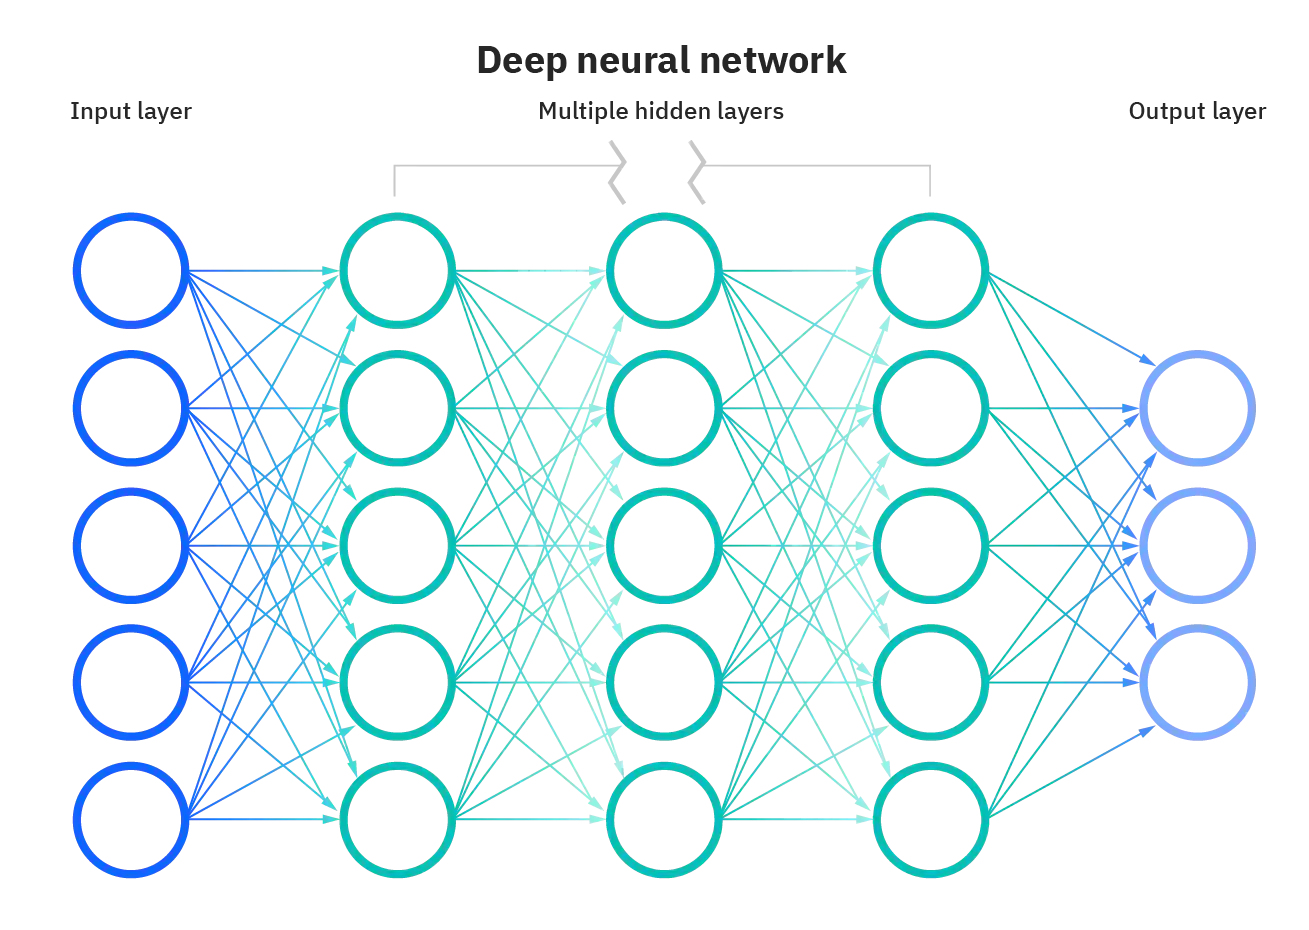
\includegraphics[width=0.75\textwidth]{{/Users/connor/Google Drive/Documents/University/Courses/2020-21/Finance 788/finance-honours/doc/reports/images/neural-network}.png}
    \caption{Standard Neural Network Topography (Source: IBM)}
    \label{fig:neural-network}
\end{figure}
The dots and lines represent nodes and connections between nodes, respectively.
The architecture of the network is derivative of intended use.
Figure \ref{fig:neural-network-configuration} illustrates the required configuration for evaluating excess returns.
$N(x,y)$ represents the yth node in xth layer.
\textbf{z} = $\sum_{a = 1}^{189} w_{(n,a,b)}x_{(n,a,b)} (= \textbf{w}^{T} \cdot \textbf{x})$ is the dot product between all outputs (x) and connection weights (w) from the nth layer, between all nodes a and b connecting layers n and n+1, respectively.
The use of dense layers deeply connects two layers where each node recieves an input from the previous layer.
The single dropout layer randomly sets input units to 0 with a frequency of rate = 50\% at each step during training time. Inputs not set to 0 are scaled up by 2 ($\frac{1}{(1-(rate = 0.5))}$ to leave the sum over all inputs unchanged.
The inclusion of a dropout layer helps prevent overfitting.
Hidden layers and output later use ReLU \ref{relu-activation-function} and linear \ref{linear-activation-function} activation functions, respectively.
An ouput linear activation (\ref{linear-activation-function}) is the most suitable for regression, predicting values ($Prediction_{k}$) between ($-\infty,\infty$) directly.
\newpage
\begin{figure}[H]
	\centering
	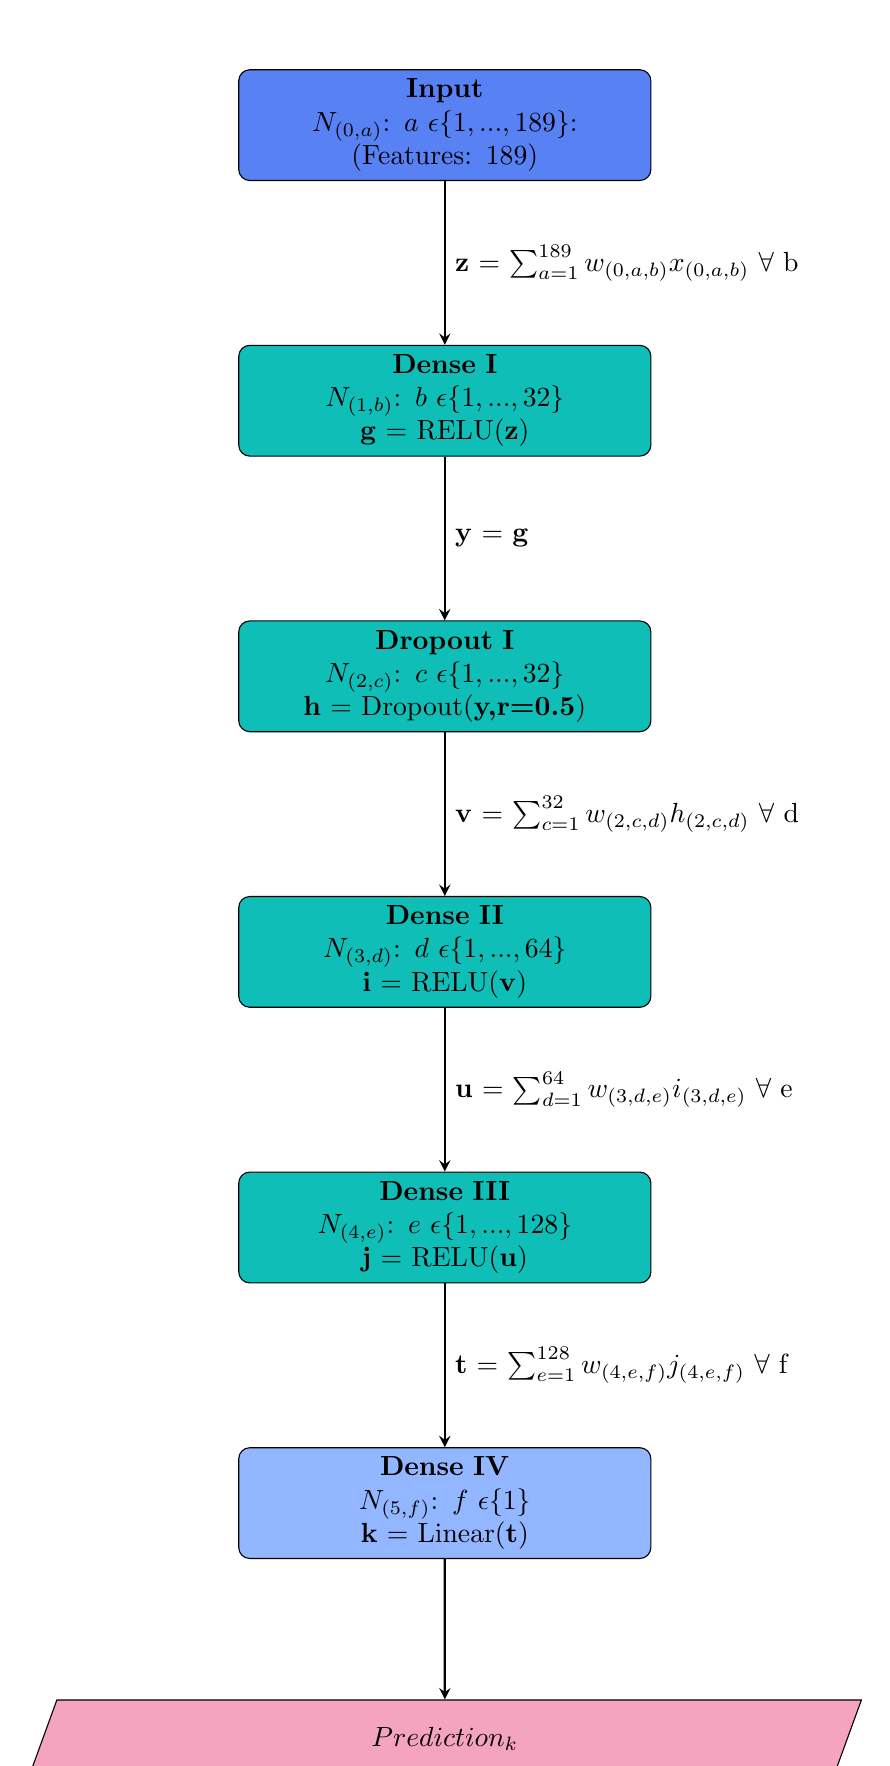
\begin{tikzpicture}[node distance=2cm]
	\node (in) [inputs] {\textbf{Input} \\ \text{$N_{(0,a)}$: \textbf{$a$ $\epsilon \{1,...,189 \}$}}: \\ (Features: 189)};
	\node (hidden1) [hiddenlayer, below of=in, yshift=-1.5cm] {\textbf{Dense I} \\ \text{$N_{(1,b)}$: \textbf{$b$ $\epsilon \{1,...,32 \}$}} \\ \textbf{g} = RELU(\textbf{z})};
	\node (hidden2) [hiddenlayer, below of=hidden1, yshift=-1.5cm] {\textbf{Dropout I} \\ \text{$N_{(2,c)}$: \textbf{$c$ $\epsilon \{1,...,32 \}$}}\\ \textbf{h} =  Dropout(\textbf{y,r=0.5})};
	\node (hidden3) [hiddenlayer, below of=hidden2, yshift=-1.5cm] {\textbf{Dense II} \\ \text{$N_{(3,d)}$: \textbf{$d$ $\epsilon \{1,...,64 \}$}} \\ \textbf{i} = RELU(\textbf{v})};
	\node (hidden4) [hiddenlayer, below of=hidden3, yshift=-1.5cm] {\textbf{Dense III} \\ \text{$N_{(4,e)}$: \textbf{$e$ $\epsilon \{1,...,128 \}$}} \\ \textbf{j} = RELU(\textbf{u})};
	\node (output) [outputlayer, below of=hidden4, yshift=-1.5cm] {\textbf{Dense IV} \\ \text{$N_{(5,f)}$: \textbf{$f$ $\epsilon \{1\}$}} \\ \textbf{k} = Linear(\textbf{t})};
	\node (predict) [predict, below of=output, yshift=-1cm] {\textbf{$Prediction_{k}$}};
	\draw [arrow] (in) -- node[anchor=west] {\textbf{z} = \text{$\sum_{a = 1}^{189} w_{(0,a,b)}x_{(0,a,b)}$} \text{$\forall$ b}} (hidden1);
	\draw [arrow] (hidden1) -- node[anchor=west] {\textbf{y} = \textbf{g}} (hidden2);
	\draw [arrow] (hidden2) -- node[anchor=west] {\textbf{v} = \text{$\sum_{c = 1}^{32} w_{(2,c,d)}h_{(2,c,d)}$} \text{$\forall$ d}} (hidden3);
	\draw [arrow] (hidden3) -- node[anchor=west] {\textbf{u} = \text{$\sum_{d = 1}^{64} w_{(3,d,e)}i_{(3,d,e)}$} \text{$\forall$ e}} (hidden4);
	\draw [arrow] (hidden4) -- node[anchor=west] {\textbf{t} = \text{$\sum_{e = 1}^{128} w_{(4,e,f)}j_{(4,e,f)}$} \text{$\forall$ f}} (output);
	\draw [arrow] (output) -- node[anchor=west] {} (predict);
	\end{tikzpicture}
	\caption{Neural Network Configuration}
    \label{fig:neural-network-configuration}
\end{figure}
\newpage
\subsubsection{Loss Functions}
Loss functions map an event or variable set, onto a real number, intuitively representing some loss, associated with the event e.g., difference between predicted and realised excess returns.
Optimisation algorithms seek to minimise loss functions by finding an exact analytical solution, or applying numerical methods to find an approximate solution, terminating after meeting exit criteria, when an analytical solution is not possible.
The training and evaluation of accurate neural networks uses this method.\footnote{The optimisation algorithm is synonymous with the training algorithm in section (\ref{mlp-math}).}
The configured neural network (figure \ref{fig:neural-network-configuration}) uses a stochastic gradient descent (SGD) algorithm (\ref{sgd}).

The relative performance between conventional minimisation loss functions, and maximisation of hedge portfolio excess returns, relies on comparing derivatives to these objectives.
The mathematical rigor and suitability of the OLS estimator (\ref{ols}) informs the widespread use of OLS regressions, and minimisation of sum of least squares, in prior asset pricing literature.
The proposition of three loss functions follow:
\singlespacing
\begin{enumerate}
	\item \textbf{In-Built Mean Square Error}: Optimized for neural networks in Tensorflow. \footnote{\href{https://www.tensorflow.org/}{activation-functionPython library for neural network modelling from Google}}
	\item \textbf{Custom Mean Square Error}: Confirm presence of automatic differentiation functionalities in Tensorflow.
	\footnote{A set of techniques to evaluate the derivative of a function specified by a computer programme,
	exploiting the sequential nature of elementary arithmetic operation and functions, repeatedly applying the chain rule in both forward and backward accumulations to compute gradients.
	Automatic differentiation solves code inefficiencies and round off error issues associated with symbolic and numerical differentiation methods, while easily calculating higher order derivatives, and partial derivatives with many inputs.}
	\item \textbf{Custom Hedge Portfolio}: A non-convex function seeking to maximise hedge portfolio returns with hedge portfolio weights determined by a monotonic ranking function mapping.
	The selected mapping weights individual equities by the proportion of their contributions to aggregate returns of all equities in a given month, considering all equities in the portfolio.
	Section \ref{hedge-portfolio-derivation} elaborates on hedge portfolio theory and formulation.
\end{enumerate}
Section \ref{loss-function-formulation} describes both mean squared error and hedge portfolio loss function formulation.
Best practice training, validation, and testing practice succeed configuration with one iteration per loss function.
The deployment of thirty epochs, shuffling of instances prior to every epoch run, and use of early stopping procedures in validation, help prevent over and under fitting.
\subsubsection{Performance Metrics}
Performance metrics inform comparisons between loss functions, to assess relative performance, after successfully training and validating a deep neural network for each loss function.
Methods for performance metrics inception and formulation follow:
\singlespacing
\begin{enumerate}
	\item The trained models predict one month lead excess returns for each instance (firm-year observation) in the testing dataset.
	\item Standard monthly sorts of predicted one month lead excess returns form standard decile ten (top 10\%) minus decile one (bottom 10\%) hedge portfolios returns per month.
	\item Use hedge portfolio to calculate the mean across all months, sharpe ratio, and treynor ratio \footnote{Uses the estimation for systematic risk from the CAPM OLS estimator}.
	\item Learning curves validate model representation.
	\item Ordinary least squares regression incorporating Newey-West estimators, (\cite{newey1987hypothesis})
	\footnote{The estimator aims to ensure autocorrelation and heteroskedasticity consistency for the regressions of time-series panel data}.
	regress: 
	\begin{itemize}
		\item Realised one month lead excess return on predicted one month lead excess return
		\item Realised hedge portfoliio excess return on predicted one month lead excess return 
		\item Hedge portfolio returns on monthly Fama-French factors, \footnote{https://mba.tuck.dartmouth.edu/pages/faculty/ken.french/data\_library.html} to find alpha in CAPM, FF3, FF4, and FF5 models (\ref{apt}).
	\end{itemize}
	\item Supplementary to OLS, Fama-MacBeth (\cite{fama1973risk})
	\footnote{Adjusted for clustered covariance with entity and time fixed effect. Standard Fama-MacBeth regressions only correct standard error for cross-sectional variation, omitting time-series autocorrelation.
	Standard forms suffice when using daily or weekly returns (and by extension, prices) as time-series correlation is weak.
	Stronger time-series autocorrelations may exist during longer period. Therefore, one month lead excess returns neccessitate time-series correction.}
	regressions validate OLS estimations. 
\end{enumerate}
\doublespacing
\newpage
\section{Results}
\subsection{Main Findings}
Table \ref{plfpe} summarises main findings
	\begin{table}[H]
		\centering
		\begin{tabular}{||c|c|c|c||}
			\hline
			Result & $MSE_{TF}$($\hat{y}$,y) & $MSE$($\hat{y}$,y) & HP($\hat{y}$)\\ [0.5ex]
			\hline \hline
			$\theta_{(Final)}$ & & & \\
			\hline
			$\lambda_{(Final)}$ & & & \\
			\hline \hline
			$\mu_{(HP)}$ & & & \\
			\hline
			$\alpha_{(HP,CAPM)}$ & & & \\
			\hline
			$\alpha_{(HP,FF3)}$ & & & \\
			\hline
			$\alpha_{(HP,FF4)}$ & & & \\
			\hline
			$\alpha_{(HP,FF5)}$& & &\\
			\hline
			$SR_{HP}$& & &\\ 
			\hline
			$TR_{HP}$ & & & \\ 
			\hline
		\end{tabular}
	\caption{Summary of Main Findings}
	\label{results summary}
\end{table}
\subsection{Performance Matrix}
\begin{tabular}{lrrr}
\toprule
     Loss Function &  HP Mean &  Sharpe Ratio &  Treynor Ratio \\
\midrule
mean\_squared\_error & 0.505614 &      3.628857 &      -6.425331 \\
        custom\_mse & 0.417429 &      3.462801 &     -11.406585 \\
         custom\_hp & 0.134763 &      3.673352 &       2.903001 \\
\bottomrule
\end{tabular}

.tex}
\cite{hlavac2018stargazer} enables the tables in the regression analysis.
\newpage
\subsection{Model Accuracy}
Section \ref{model-training-validation-performance} illustrates relative training and validation performance between loss functions.
\subsection{Learning Curves}

\subsubsection{Model Loss}
Table X illustrates the performance of each model during training, validation, and testing.
Table \ref{test-model-predict} informs the accruracy of predictions 
\begin{table}[H] \centering
  \begin{tabular}{@{\extracolsep{5pt}}lccc}
    \\[-1.8ex]\hline
    \hline                                                                                                                                                        \\[-1.8ex]
                        & \multicolumn{3}{c}{\textit{Dependent variable: One Month Lead Excess Returns (OMLER)}} \
    \cr \cline{2-4}
    \\[-1.8ex] &  MSE & MSE (Custom) & Hedge Portfolio \\
    \hline                                                                                                                                                        \\[-1.8ex]
    Predicted (OMLER)   & 0.129$^{***}$                                                                             & 0.238$^{***}$        & -1.319$^{***}$       \\
                        & (0.004)                                                                                   & (0.005)              & (0.210)              \\
    \hline                                                                                                                                                        \\[-1.8ex]
    Observations        & 531,461                                                                                   & 531,461              & 531,461              \\
    $R^2$               & 0.012                                                                                     & 0.042                & 0.001                \\
    Adjusted $R^2$      & 0.012                                                                                     & 0.042                & 0.001                \\
    Residual Std. Error & 0.137                                                                                     & 0.135                & 0.137                \\
                        & (df = 531460)                                                                             & (df = 531460)        & (df = 531460)        \\
    F Statistic         & 1188.583$^{***}$                                                                          & 2037.581$^{***}$     & 39.655$^{***}$       \\
                        & (df = 1.0; 531460.0)                                                                      & (df = 1.0; 531460.0) & (df = 1.0; 531460.0) \\
    \hline
    \hline                                                                                                                                                        \\[-1.8ex]
    \textit{Note:}      & \multicolumn{3}{r}{$^{*}$p$<$0.1; $^{**}$p$<$0.05; $^{***}$p$<$0.01}                                                                    \\
  \end{tabular}
  \caption{Predictability of One Month Lead Portfolio Excess Returns}
\end{table}
.tex}
Fama MacBeth Regressions using individual securities.
PooledOLS replaces Fama MacBeth in this instance.
\subsection{Hedge Portfolio Performance}

\subsubsection{Inbuilt Mean Square Error}
\subsubsection{Custom Mean Square Error}
\subsubsection{Custom Hedge Portfolio}
\newpage
\section{Discussion}
\section{Conclusion (2 pages)}
\subsection{Contributions}
\subsection{Further Research}
\subsection{Limitations}
Further research will rely on addressing severals limitation.
\subsubsection{Resources}
The lack of resources to explore the entire dataset within reasonable timeframes, and at reasonable costs.
The most material inhibitions are the inability to explore all 400 factors for all size groupings, the reduction in level of precision for numerical features, and
the ability to shuffle training sets at lengths greater than or equal to the input sets.
\newpage
\printbibliography
\newpage
\section{Appendix}
\subsection{Mathematics}
\subsubsection{Equations \& Derivations}
\subsubsection{Hedge Portfolio} \label{hedge-portfolio-derivation}
Hedge portfolios rely on monotonic ranking functions for optimisation as their monotonic nature preserves or reverses a given ordered set.
The analysis cross-section of one-month lead portfolio excess returns using monotonic functions 
\begin{align}
	R(y_{i,t}) \numberthis \label{ranking-function}
\end{align}
The ranking function (R($y_{i,t}$)) and thresholds (u,v) form subsets of long and short portfolios.
Long (L) or Short (S) sets include excess returns conditioned on the associated monotonic ranking given a threshold, bound by the cardinality of the excess return vector ($|y|$).
The subsequent truth sets mathematically express aforementioned time-series hedge portfolios.
\begin{align*}
	L &= \{ y_{i,t} | R(y_{i,t})\leq u\}\\
	S &= \{ y_{i,t} | R(y_{i,t})\geq v\}\\
	0 & < u \leq |y|\\
	0 & < v \leq |y|\\
	u & < v
\end{align*}
Equation \ref{htls} describes hedge portfolio lead excess returns ($H_t$) at a given time (t).
\begin{align}
	H_t &= \frac{1}{|L|}\sum_{i\epsilon L} y_{i,t} - \frac{1}{|S|}\sum_{i\epsilon S} y_{i,t} \label{htls}
\end{align}
Figure \ref{fig:mrf}) illustrates an approximate linear monotonic ranking function with a sample of 100 uniformly distributed excess returns  between -10\% and 10\%.
Boundary conditions u and v are set to 20 and 80 , respectively.
Subsequently, excess returns above (below) the green (blue) dotted line belong to the long (L) (short (S)) set. 
\begin{figure}[H]
    \centering 
    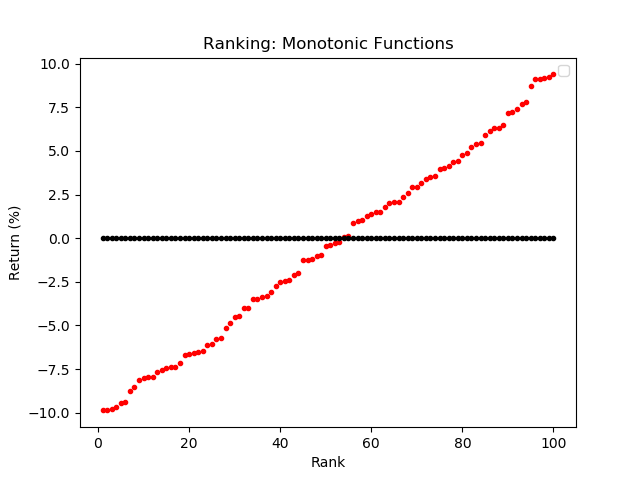
\includegraphics[width=\textwidth]{{/Users/connor/Google Drive/Documents/University/Courses/2020-21/Finance 788/finance-honours/results/plots/monotonic-ranking}.png}
    \caption{Approximate Linear Monotonic Ranking Function}
    \label{fig:mrf}
\end{figure}
The permutations in monotonic ranking functions, and subsequent hedge portfolios, are endless. 
This research essay develops a monotonic ranking function proportionally weighting one month lead excess returns (\ref{w1}).
Therefore, equation \ref{pwlf} defines the loss function.
\begin{align*}
	R(\hat{y}) &= W \numberthis \label{w1}\\
	W&:= \frac{\hat{y}}{\vec{\textbf{1}}\hat{y}}\\
	\hat{y} &= X^{T} \hat{\theta}\\
	f_{\hat{\theta}}(X) &= (\frac{X^{T} \hat{\theta}}{\vec{\textbf{1}}X^{T} \hat{\theta}})^\top X^{T} \hat{\theta} \numberthis \label{pwlf}
\end{align*}
The above loss function is differentiable using symbolic mathematic as shown in equation \ref{pdewlf}.
\begin{align*}
	\frac{\partial f_{\hat{\theta}}(X)}{\partial \hat{\theta}} &= \frac{\partial ((\frac{X^{T} \hat{\theta}}{\vec{\textbf{1}}X^{T} \hat{\theta}})^\top X^{T} \hat{\theta})}{\partial \hat{\theta}} \\
	\frac{\partial (f_{\hat{\theta}}(X))}{\partial \hat{\theta}}  &= \frac{1}{(\hat{\theta}^\top X \vec{1})} X X^\top \hat{\theta} +\frac{1}{\vec{1}X^\top \hat{\theta}} XX^\top \hat{\theta} -\frac{1}{(\hat{\theta}^\top X \vec{1})^{2}} \hat{\theta}^\top XX^\top \hat{\theta} X \vec{1} \numberthis \label{pdewlf}
\end{align*}
Subsection \ref{sec:mlo} explains the theory supporting loss minimisation.
Applying gradient descent methods to the product of  the loss function and scaler of -1 transforms the minimisation to maximisation.
This transformation leads to finding the argmax of maximisation function with respect to $\hat{\theta}$ (\ref{argmax}).
The aforementioned transformation is simply and suitable for exploration in the context of the research intent.
More sophisticated methods exist for maximisation such as reinforcement learning (\ref{rifml}).
\begin{align*}
	\argmax_{\hat{\theta}} &: (\frac{X^{T} \hat{\theta}}{\vec{\textbf{1}}X^{T} \hat{\theta}})^\top X^{T} \hat{\theta} \numberthis \label{argmax}
\end{align*}
\subsubsection{Loss Functions}\label{loss-function-formulation}
Equations \ref{f-mse} and \ref{f-hp} show the loss functions calculating mean squared errors and aforementioned hedge portfolios, respectively.
Equations \ref{argmin-mse} and \ref{argmax-hp} illustrate optimisation objectives for mean squared error and hedge portfolio loss functions, respectively. \footnote{$\argmax_{\hat{\theta}}: (f_{\hat{\theta}}(X)) \equiv \argmin_{\hat{\theta}}: (-f_{\hat{\theta}}(X))$}
Equations \ref{pd-mse} and \ref{pd-hp} describe the partial derivative functions for both mean squared error and hedge portfolio loss functions, respectively.
The global optimum for both functions is the combination of parameters ($\hat{\theta}$) setting the partial derivative to zero. 
The first is trivial in an analytical form. The second is non-trivial, requiring symbolic, numerical, or automatic methods.
The immediate code listings show the translation of loss functions mathematical expressions (\ref{f-mse} and \ref{f-hp}) into tensor compatible formats for analysis.
\begin{multicols}{2}
\noindent
	\begin{equation}
		f_{\hat{\theta}}(y, X)= \frac{\vec{1}}{\vec{1}^{T}\vec{1}} (\textbf{y} - X^{T}\hat{\theta})^{\circ 2} \numberthis 
		\label{f-mse}
	\end{equation}
	\begin{equation}
		f_{\hat{\theta}}(X)= (\frac{X^{T} \hat{\theta}}{\vec{\textbf{1}}X^{T} \hat{\theta}})^\top X^{T} \hat{\theta} \numberthis
		\label{f-hp}
	\end{equation}
\end{multicols}
\begin{multicols}{2}
	\noindent
		\begin{equation}
		\argmin_{\hat{\theta}}: (f_{\hat{\theta}}(y, X)) \numberthis 
		\label{argmin-mse}
	\end{equation}
	\begin{equation}
		\argmax_{\hat{\theta}}: (f_{\hat{\theta}}(X)) \numberthis 
		\label{argmax-hp}
	\end{equation}
\end{multicols}
\begin{equation}
	\frac{\partial f_{\hat{\theta}}(y, X)}{ \partial \hat{\theta}} = \frac{\vec{1}}{\vec{1}^{T}\vec{1}} (-2(\textbf{y}-X^{T} \hat{\theta})^{\circ 1}) \numberthis 
	\label{pd-mse}
\end{equation}
\begin{equation}
	\frac{\partial (f_{\hat{\theta}}(X))}{\partial \hat{\theta}}  = \frac{1}{(\hat{\theta}^\top X \vec{1})} X X^\top \hat{\theta} +\frac{1}{\vec{1}X^\top \hat{\theta}} XX^\top \hat{\theta} -\frac{1}{(\hat{\theta}^\top X \vec{1})^{2}} \hat{\theta}^\top XX^\top \hat{\theta} X \vec{1} \numberthis 
	\label{pd-hp}
\end{equation}
\begin{lstlisting}[language=Python, caption = Custom Mean Squared Error Implementation]
	class custom_mse(tf.keras.losses.Loss):
		def __init__(self, extra_tensor=None, reduction=tf.keras.losses.Reduction.AUTO, name='custom_mse'):
			super().__init__(reduction=reduction, name=name)
			self.extra_tensor = extra_tensor

		def call(self, y_true, y_pred):
			extra_tensor = self.extra_tensor
			loss = K.mean(K.square(y_pred - y_true))
			return loss
\end{lstlisting}
\begin{lstlisting}[language=Python,caption = Custom Hedge Portfolio Implementation]
	class custom_hp(tf.keras.losses.Loss):
		def __init__(self, extra_tensor=None, reduction=tf.keras.losses.Reduction.AUTO, name='custom_hp'):
			super().__init__(reduction=reduction, name=name)
			self.extra_tensor = extra_tensor

		def call(self, y_true, y_pred):
			extra_tensor = self.extra_tensor
			# Calculates sum over vector tensors
			y_true_sum = K.sum(y_true)
			y_pred_sum = K.sum(y_pred)
			#
			y_true_weights = (y_true/y_true_sum)
			y_pred_weights = (y_pred/y_pred_sum)
			# Transpose the weights
			y_true_transposed = K.transpose(y_true_weights)
			y_pred_transposed = K.transpose(y_pred_weights)
			# Multiply by the weights
			y_true_loss = K.dot(y_true_transposed, y_true)
			y_pred_loss = K.dot(y_pred_transposed, y_pred)
			loss = -1*(y_pred_loss)
			return loss
\end{lstlisting}

\subsection{Stochastic Gradient Descent}\label{sgd}
Firstly, SGD finds loss function partial derivatives, with the respect to the parameter in a predictive model.
Secondly, the exploration of epochs update parameters using a learning rate, moving away from the partial derivatives, until settling in a minimum as a potential solution.
Several methods aid escape from local minima to continue searching for global minimum solutions, depending on the algorithm. 
The below illustrates the use of mean squared error as a loss function, on a linear model, where SGD would adjust both intercept and co-efficient parameters, in order to find the argmax of the loss function.
\\
Equations for linear model (\ref{lm}) and mean squared error (\label{mse}).
\begin{align*}
	\hat{y} &= mx_i + b \numberthis \label{lm}\\
	f(y,(mx_{i} + b)) &= \frac{1}{n} \sum_{i=1}^{n}(y_i - (mx_{i} + b))^{2} \numberthis 
\end{align*}
Partial derivatives of parameters m (\ref{pdmsem}) and b (\ref{pdmseb}), respectively.
\begin{align*}
	\frac{\partial f(y,(mx_{i} + b)}{ \partial m} &= \frac{1}{n} \sum_{i=1}^{n}-2x_{i}(y_i - (mx_{i} + b))^{2} \numberthis \label{pdmsem}\\
	\frac{\partial f(y,(mx_{i} + b)}{ \partial b} &= \frac{1}{n} \sum_{i=1}^{n}-2(y_i - (mx_{i} + b))^{2} \numberthis \label{pdmseb}
\end{align*}
\subsection{Ordinary Least Squares (OLS)}\label{ols}
The OLS regression is the most prominent statistical model in asset pricing theory.
Rosenfeld (\citeyear{olsmf}) summarises OLS.
The composition of the true OLS (\ref{true-ols}) model includes four components.
Firstly, \textbf{X}, an n x k matrix of k independent variables for n observations.
Secondly, \textbf{y}, an n x 1 vector of observation on the dependent variable.
Thirdly, \textbf{$\epsilon$}, an n x 1 vector of unexplained error.
Lastly, $\theta$, a k x 1 vector of parameters to be estimated.
\begin{align*}
	y &= X\theta + \epsilon \numberthis \label{true-ols}
\end{align*}
\subsubsection{Estimation Criteria}
The criteria to obtain the parameter estimate ($\hat{\theta}$) relies on the minimisation of the sum of squared residuals (\ref{ssr}).
We highlight the observed residuals (e) are distinct from unexplained disturbances ($\epsilon$).
Equation \ref{res} derives residuals by taking the difference between observations based on parameter estimates.
\begin{align*}
	\sum & e_i^2  \numberthis \label{ssr}\\
	e = y & - X \hat{\theta} \numberthis \label{res}
\end{align*}
Expanding the quadratic $e^{T}e$ after substituting in equation \ref{res} leads to the alternative expression of the sum of squared residuals in equation \ref{ssrm}.
Minimizing the sum of square residuals requires taking the partial derivative of equation \ref{ssrm} with respect to the estimated parameters (equation) using matrix differentiation (\ref{ssrmd}).
It is imperative X has full rank where all vectors in the matrix are linearly independent, validating both the presence of a positive definite matrix and minimum.
\begin{align*}
	e^{T}e &= y^{T}y - 2\hat{\theta}^{T}X^{T}y + \hat{\theta}^{T}X^{T}\hat{\theta}X \numberthis \label{ssrm}\\
	\frac{\partial e^{T}e}{\partial \hat{\theta}} &= - 2X^{T}y + 2X^{T}X\hat{\theta} =0 \numberthis \label{ssrmd}
\end{align*}
We find the expression for the Ordinary Least Squares (OLS) estimator (\ref{OLSD}) after rearranging equation \ref{ssrmd} to normal form, utilizing inverse matrices to form identity matrices, and simplifying.
\begin{align*}
	2X^{T}X\hat{\theta} &= 2X^{T}y \\
	(X^{T}X)^{-1}(X^{T}X)\hat{\theta} &= (X^{T}X)^{-1}X^{T}y \\
	I\hat{\theta} &= (X^{T}X)^{-1}X^{T}y \\
	\hat{\theta} &= (X^{T}X)^{-1}(X^{T}y) \numberthis \label{OLSD}\\
\end{align*}
Therefore, we can use the OLS estimator to make predictions with OLS (\ref{OLS}).
\begin{align*}
	\hat{y} &= X^{T} \hat{\theta} \numberthis \label{OLS}
\end{align*}
\subsubsection{Properties of OLS Estimators}
There are six key properties in addition to the satisfaction in minimizing the summation of squared residuals.
\begin{enumerate}
	\item The residuals are uncorrelated with the observed values of X i.e., $X^{T}e=0$.
	\item The sum of the residuals is zero i.e., $\sum e_i=0$.
	\item The sample mean of the residuals is zero i.e., $\bar{e} = \frac{\sum e_i}{n} = 0$.
	\item The regression hyperplane passes through the means of observed values i.e., $\frac{e} = \frac{y - X\theta}{n} = 0$. Since $\bar{e} = 0$ assumed, it is implied $\bar{y}=\bar{x}\bar{\theta}$.
	\item The residuals are uncorrelated with the predicted y i.e., $\hat{y} = X\hat{\theta}$, $\hat{y}^{T}e = (X\hat{\beta})^{T}e = b^{T}X^{T}e = 0$ 
	\item The mean of $\hat{y}$ for the sample will equal the mean of the y.
\end{enumerate}
\subsubsection{The Gauss-Markov Theorem}
However, OLS makes Gauss-Markov assumptions about the true model to make inferences regarding $\beta$ from $\hat{\beta}$.
The intention of the Gauss-Markov Theorem, conditional on the below assumptions, states the OLS estimator is the best linear, unbiased, and efficient estimator: 
\begin{align*}
	y &= x\beta + \epsilon\\
	E[\epsilon|X] &= 0 \numberthis \label{gma3}\\
	E(\epsilon \epsilon^{T}|X) &= \Omega = \sigma^{2}I \numberthis \label{gma4}\\
	\epsilon &| X ~ N[0,\sigma^{T}I] \text{ (hypothesis testing)}
\end{align*}
\begin{itemize}
	\item X is an n x k matrix of full rank
	\item X must be generated randomly, or fixed, by a mechanism uncorrelated to disturbances.
\end{itemize}
Equation \ref{gma3} implies $E(y) = X\beta$ as no observations of the independent variables convey any information about the expected values of the disturbances.
Equation \ref{gma4} captures homoskedasticity and no autocorrelation assumptions.
\newpage
\begin{landscape}
\subsection{Model Training \& Validation Performance} \label{model-training-validation-performance}
\begin{figure}[H]
    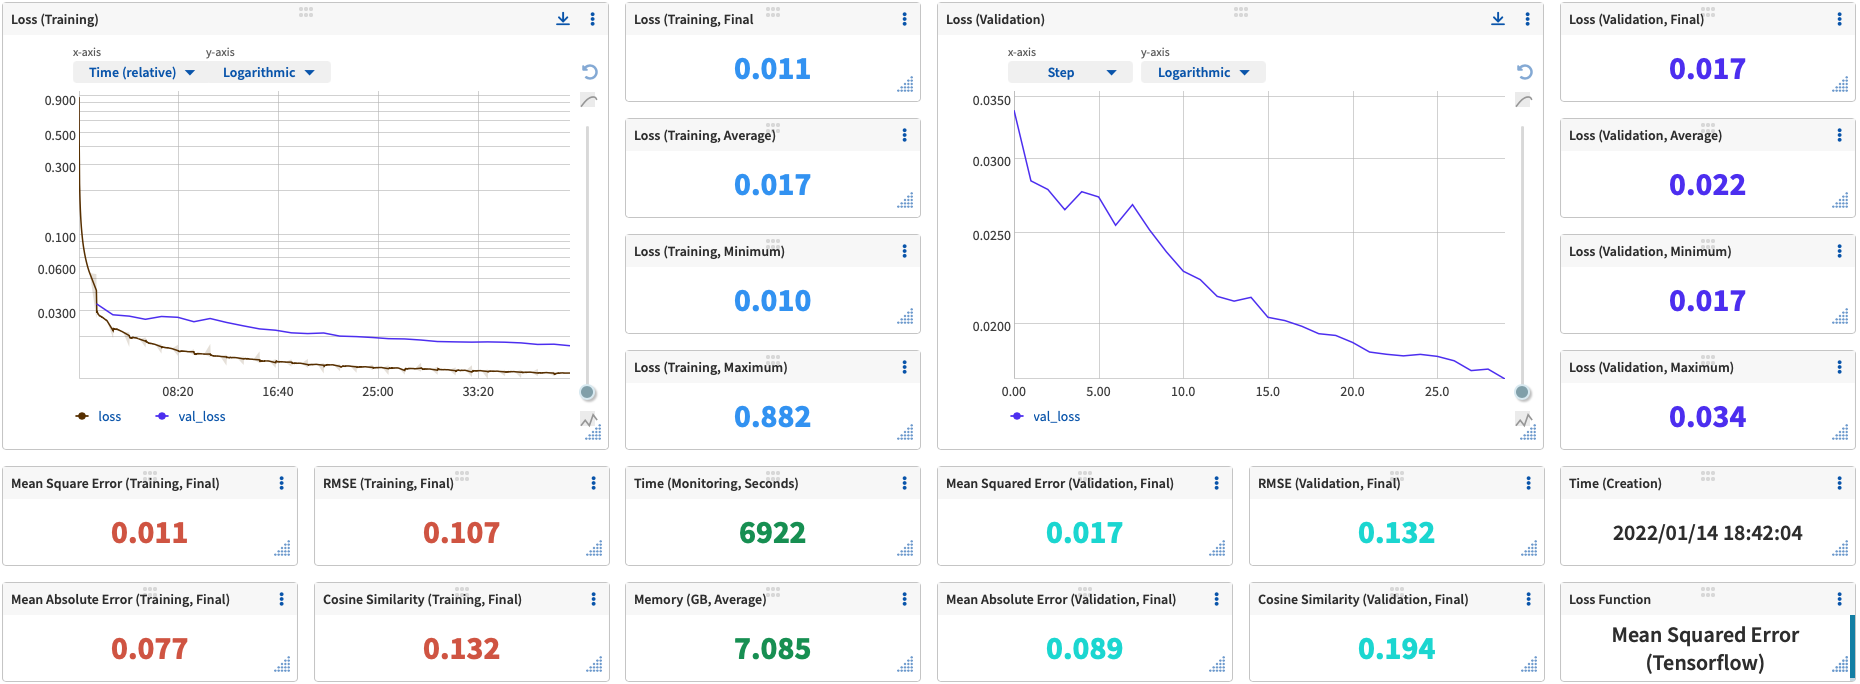
\includegraphics[width=1.5\textwidth]{mean-squared-error.png}
    \caption{Performance: In-Built Mean Square Error}
    \label{fig:mse-tf-performance}
\end{figure}
\begin{figure}[H]
    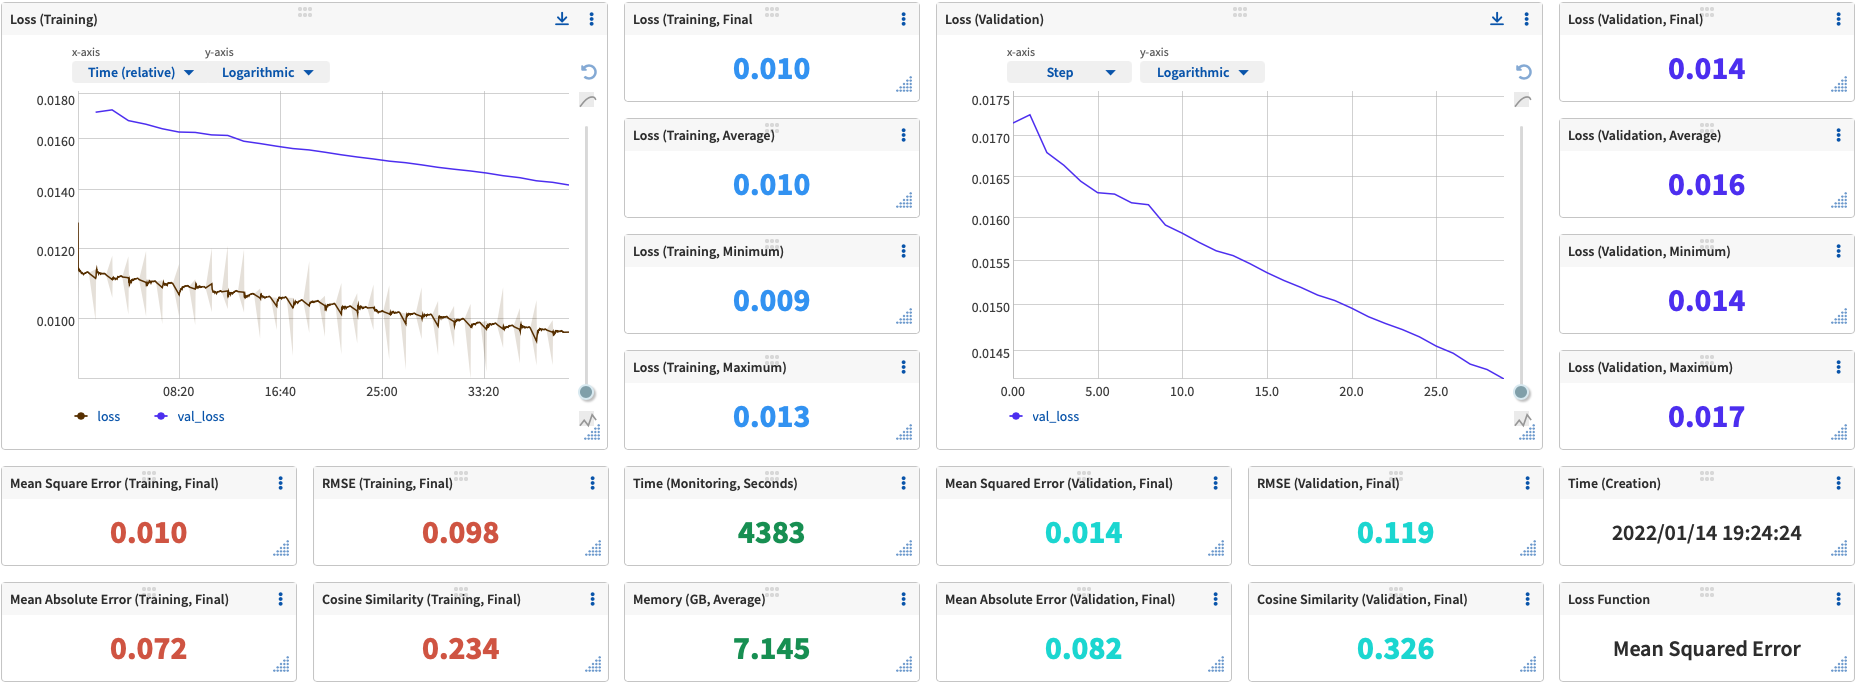
\includegraphics[width=1.5\textwidth]{custom-mse.png}
    \caption{Performance: Custom Mean Square Error}
    \label{fig:mse-performance}
\end{figure}
\begin{figure}[H]
    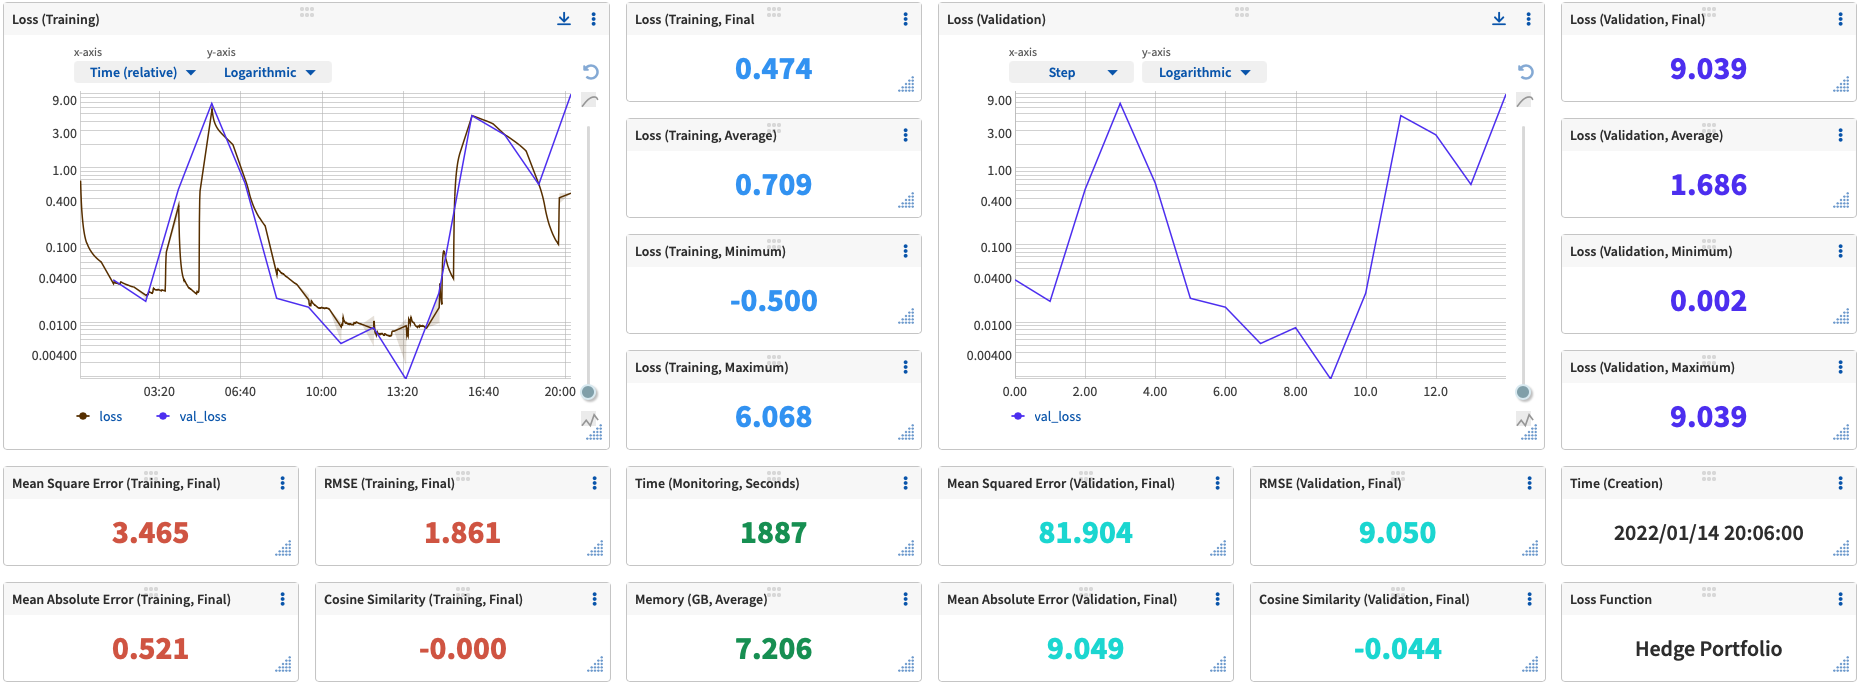
\includegraphics[width=1.5\textwidth]{custom-hp.png}
    \caption{Performance: Custom Hedge Portfolio}
    \label{fig:hp-performance}
\end{figure}
\end{landscape}
\subsection{Asset Pricing Models}\label{apm}
\subsubsection{Capital Asset Pricing Model}
\begin{align*}
	R_{i,t} - R_{f,t} &= \alpha_{i,t} + \beta_{i,t}^{1}(R_{M,t}-R_{f,t}) \numberthis \label{capm}
\end{align*}
\subsubsection{Fama-French Factor Models}
\begin{align*}
	R_{i,t} - R_{f,t} &= \alpha_{i,t} + \beta_{i,t}(R_{M,t}-R_{f,t}) \numberthis \label{ff3}\\
	R_{i,t} - R_{f,t} &= \alpha_{i,t} + \beta_{i,t}(R_{M,t}-R_{f,t}) \numberthis \label{ff5}
\end{align*}
where
\begin{itemize} 
	\item $R_{i,t} - R_{f,t}$: Portfolio Excess Return on the market for a given portfolio and time, value-weighted using all incorporated US CRSP firms incorporated in the US, listed on the NYSE, AMEX, or NASDAQ.
	\item $\alpha_{i,t}$: Jensen's alpha indicating mispricing in the asset.
	\item $\beta_{t}^{1}$: Market Risk Factor (co-efficient)
	\item $\beta_{t}^{1}$: Size Factor (co-efficient)
	\item $\beta_{t}^{2}$: Value Factor (co-efficient)
	\item $\beta_{t}^{2}$: Value Factor (co-efficient)
	\item $\beta_{t}^{3}$: Profitability Factor (co-efficient)
	\item $\beta_{t}^{4}$: Investment Factor (co-efficient)
	\item $(R_{M,t}-R_{f,t})$: Market Risk Premium
	\item $SMB_{t}$: Size Premium (small minus big) is the difference in average return between nine small stock and nine large value-weighted portfolios.
	\item $HML_{t}$: Value Premium (high minus low) is the difference in average return between two value and two growth value-weighted portfolios.
	\item $RMW_{t}$: Profitability Premium (robust minus weak) is the difference in average return between two robust operating profitability and two weak operating profitability value-weighted portfolios.
	\item $CMA_{t}$: Investment Premium minus aggressive is the difference in average return on the two conservative and two aggressive investment portfolios
\end{itemize}
\subsubsection{Fama-MacBeth Regressions}
\begin{align*}
	R_{n,t} &= \alpha_{n} + \sum_{f=1}^{F} \beta_{n,F_{f}}F_{f,t} + \epsilon_{n,t} \numberthis \label{fb1} \\
	&\forall \text{  }n\epsilon\{1,...,N\}\\
	R_{i,t} &= \gamma_{t,0} + \sum_{f=1}^{F} \gamma_{t,f}\hat{\beta_{i,F_{f}}} + \epsilon_{i,t} \numberthis \label{fb2} \\
	&t\epsilon\{1,...,N\}
\end{align*}
Where
\begin{itemize}
	\item $R_{n,t}$: Return for an asset (n) at a time (t).
	\item $\alpha_{n}$: Jensen's alpha for an asset (n) implying mispricing.
	\item $\beta_{n,F_{f}}$: An asset's (n) exposure to a factor (f)
	\item $\hat{\beta_{i,F_{f}}}$: Estimated factor loading for a factor (f) from regression of asset (i)
	\item $F_{f,t}$: Risk factor (f) at a given time (t) e.g., SMB, HML etc.,
	\item $\epsilon_{n,t}$: Residual for an asset at a time (t)
	\item $\gamma_{t,f}$: Factor pricing for a factor (f)
\end{itemize}
\subsubsection{Sharpe Ratio}
Nobel Laurette William F. Sharpe (\citeyear{sharpe1994sharpe}) introduced the Sharpe Ratio (\ref{sr}) as a measure for risk-adjusted returns,
where $\mathop{\mathbb{E}} [R_a - R_f]$ is the expectation for excess returns, and $\sigma(R_a)$ is the standard deviation of excess returns.
\begin{align*}
	SR &= \mathop{\mathbb{E}} \frac{[R_a - R_f]}{\sigma(R_a)} \numberthis \label{sr}\\
	\sigma &= \sqrt{\sum_{i=1}^{n}}\frac{(R_a) - \bar{R_a})^2}{n}
\end{align*}
\subsubsection{Treynor Ratio}
The Treynor ratio is another risk-return measure (\ref{tr}), evaluating the excess return of a portfolio per unit of systemic risk\footnote{}.
$\mathop{\mathbb{E}} [R_a - R_f]$ is the excess return on the market. $\beta_{M}$ is systematic risk
\begin{align*}
	\text{Treynor} &= \mathop{\mathbb{E}} \frac{[R_a - R_b]}{\beta_{M}} \numberthis \label{tr}\\
\end{align*}
\newpage
\subsection{Pooled Ordinary Least Square Regressions} \label{polsr}
\subsubsection{In-Built Mean Square Error}
\begin{center}
\begin{tabular}{lclc}
\toprule
\textbf{Dep. Variable:}    &  ret\_exc\_lead1m  & \textbf{  R-squared:         }   &      0.0003      \\
\textbf{Estimator:}        &     PooledOLS      & \textbf{  R-squared (Between):}  &      0.0019      \\
\textbf{No. Observations:} &       531461       & \textbf{  R-squared (Within):}   &     -0.0001      \\
\textbf{Date:}             &  Thu, Jan 13 2022  & \textbf{  R-squared (Overall):}  &      0.0003      \\
\textbf{Time:}             &      04:01:42      & \textbf{  Log-likelihood     }   &    3.008e+05     \\
\textbf{Cov. Estimator:}   &     Clustered      & \textbf{                     }   &                  \\
\textbf{}                  &                    & \textbf{  F-statistic:       }   &      147.92      \\
\textbf{Entities:}         &        7282        & \textbf{  P-value            }   &      0.0000      \\
\textbf{Avg Obs:}          &       72.983       & \textbf{  Distribution:      }   &   F(1,531460)    \\
\textbf{Min Obs:}          &       1.0000       & \textbf{                     }   &                  \\
\textbf{Max Obs:}          &       252.00       & \textbf{  F-statistic (robust):} &      10.070      \\
\textbf{}                  &                    & \textbf{  P-value            }   &      0.0015      \\
\textbf{Time periods:}     &        252         & \textbf{  Distribution:      }   &   F(1,531460)    \\
\textbf{Avg Obs:}          &       2109.0       & \textbf{                     }   &                  \\
\textbf{Min Obs:}          &       1869.0       & \textbf{                     }   &                  \\
\textbf{Max Obs:}          &       3400.0       & \textbf{                     }   &                  \\
\bottomrule
\end{tabular}
\begin{tabular}{lcccccc}
                 & \textbf{Parameter} & \textbf{Std. Err.} & \textbf{T-stat} & \textbf{P-value} & \textbf{Lower CI} & \textbf{Upper CI}  \\
\midrule
\textbf{predict} &       0.0064       &       0.0020       &      3.1733     &      0.0015      &       0.0025      &       0.0104       \\
\bottomrule
\end{tabular}
%\caption{PooledOLS Estimation Summary}
\end{center}
.tex}
\subsubsection{Custom Mean Square Error}
\begin{center}
\begin{tabular}{lclc}
\toprule
\textbf{Dep. Variable:}    &  ret\_exc\_lead1m  & \textbf{  R-squared:         }   &      0.0029      \\
\textbf{Estimator:}        &     PooledOLS      & \textbf{  R-squared (Between):}  &      0.0035      \\
\textbf{No. Observations:} &       531461       & \textbf{  R-squared (Within):}   &      0.0030      \\
\textbf{Date:}             &  Wed, Jan 12 2022  & \textbf{  R-squared (Overall):}  &      0.0029      \\
\textbf{Time:}             &      05:52:03      & \textbf{  Log-likelihood     }   &    3.015e+05     \\
\textbf{Cov. Estimator:}   &     Clustered      & \textbf{                     }   &                  \\
\textbf{}                  &                    & \textbf{  F-statistic:       }   &      1564.3      \\
\textbf{Entities:}         &        7282        & \textbf{  P-value            }   &      0.0000      \\
\textbf{Avg Obs:}          &       72.983       & \textbf{  Distribution:      }   &   F(1,531460)    \\
\textbf{Min Obs:}          &       1.0000       & \textbf{                     }   &                  \\
\textbf{Max Obs:}          &       252.00       & \textbf{  F-statistic (robust):} &      6.7467      \\
\textbf{}                  &                    & \textbf{  P-value            }   &      0.0094      \\
\textbf{Time periods:}     &        252         & \textbf{  Distribution:      }   &   F(1,531460)    \\
\textbf{Avg Obs:}          &       2109.0       & \textbf{                     }   &                  \\
\textbf{Min Obs:}          &       1869.0       & \textbf{                     }   &                  \\
\textbf{Max Obs:}          &       3400.0       & \textbf{                     }   &                  \\
\bottomrule
\end{tabular}
\begin{tabular}{lcccccc}
                 & \textbf{Parameter} & \textbf{Std. Err.} & \textbf{T-stat} & \textbf{P-value} & \textbf{Lower CI} & \textbf{Upper CI}  \\
\midrule
\textbf{predict} &       0.0449       &       0.0173       &      2.5974     &      0.0094      &       0.0110      &       0.0788       \\
\bottomrule
\end{tabular}
%\caption{PooledOLS Estimation Summary}
\end{center}
.tex}
\subsubsection{Custom Hedge Portfolio}
\begin{center}
\begin{tabular}{lclc}
\toprule
\textbf{Dep. Variable:}    &  ret\_exc\_lead1m  & \textbf{  R-squared:         }   &      0.0010      \\
\textbf{Estimator:}        &     PooledOLS      & \textbf{  R-squared (Between):}  &     -0.0060      \\
\textbf{No. Observations:} &       531461       & \textbf{  R-squared (Within):}   &      0.0007      \\
\textbf{Date:}             &  Sat, Jan 15 2022  & \textbf{  R-squared (Overall):}  &      0.0010      \\
\textbf{Time:}             &      03:35:51      & \textbf{  Log-likelihood     }   &     3.01e+05     \\
\textbf{Cov. Estimator:}   &     Clustered      & \textbf{                     }   &                  \\
\textbf{}                  &                    & \textbf{  F-statistic:       }   &      529.44      \\
\textbf{Entities:}         &        7282        & \textbf{  P-value            }   &      0.0000      \\
\textbf{Avg Obs:}          &       72.983       & \textbf{  Distribution:      }   &   F(1,531460)    \\
\textbf{Min Obs:}          &       1.0000       & \textbf{                     }   &                  \\
\textbf{Max Obs:}          &       252.00       & \textbf{  F-statistic (robust):} &      5.4613      \\
\textbf{}                  &                    & \textbf{  P-value            }   &      0.0194      \\
\textbf{Time periods:}     &        252         & \textbf{  Distribution:      }   &   F(1,531460)    \\
\textbf{Avg Obs:}          &       2109.0       & \textbf{                     }   &                  \\
\textbf{Min Obs:}          &       1869.0       & \textbf{                     }   &                  \\
\textbf{Max Obs:}          &       3400.0       & \textbf{                     }   &                  \\
\bottomrule
\end{tabular}
\begin{tabular}{lcccccc}
                 & \textbf{Parameter} & \textbf{Std. Err.} & \textbf{T-stat} & \textbf{P-value} & \textbf{Lower CI} & \textbf{Upper CI}  \\
\midrule
\textbf{predict} &      -1.3194       &       0.5646       &     -2.3369     &      0.0194      &      -2.4260      &      -0.2128       \\
\bottomrule
\end{tabular}
%\caption{PooledOLS Estimation Summary}
\end{center}
.tex}

\subsection{Technical Details}\label{technical}
\subsubsection{Organisation}
This research essay uses data science best practise (\cite{J:10}).
Data and results saved regularly and reproducible. 
Data retention in all forms receives high levels of attention. 
Project files synchonises continuously to Google Drive (\cite{Google_Drive}). 
Git (\cite{Git}) manages version control protocols for source code, data, documents, and results.
Git stores a complete history of versions using Git hashes. 
These hashes are strings unique to each state of the publicly available finance-honours repository\footnote[1]{https://github.com/CMCD1996/finance-honours}. 
Git hashes enable discretisation of finance-honours development, enabling the accessibility and recollection of all previous states given a unique git hash. 
This functionality enables reproducibility, error correction, and the ability to revert to previous models.

\subsubsection{Version Control}\label{Version Control}
Git, hosted by GitHub, provides a comprehensive set of version control technologies and range of benefits.
These technologies manage version control for the programming of approximately 40 methods, classes, and functions.
Firstly, Git enables collaborative functionalities. 
The master version of a project is accessible for all who have access to the repository. 
Each contributor can create custom copies of branches through pull requests on the master branch. 
Contributors can commit changes to custom branches and push these changes to the master branch through push requests. 
Product managers can review push requests, approving valid requests for integrating changes to the master branch. 
Collaborative efforts are possible with commit messages describing contributions from each contributor. 
This research essay has only one contributor, rendering collaborative functionalities redundant in this instance.
Git ensures the storage of code, work, and author histories.
The descriptive nature of commit logs ensures journal accuracy.

\subsubsection{Directories}
This research essay follows directory structure recommendations from Wilson et al (\citeyear{J:10}). 
Organisation is crucial as the modelling of artificial neural networks involves integrating a range of optimisation models, data files and documents.  
Directory management is most efficient and comprehensive. 
\textbf{finance-honours} is the root directory containing the following sub directories: bin, data, doc, src, and results.  
The \textbf{bin} sub directory contains external scripts and compiled programmes. 
The \textbf{data} sub directory contains all raw data associated with the project. 
The \textbf{doc} sub directory stores user guides, academic resources, research reports and project deliverables.
The \textbf{results} sub directory contains the outputs from project analysis.
The \textbf{src} sub directory stores the source code for preparing datasets, partitioning sets of geographies with varying granularities.
All files were continuously backed up using Google Drive and Git.

\subsubsection{Python}\label{python}
Python 3.9.7 is the primary programming language for this research essay. 
The language is omnipresent, widespread in software development. 
Python's language design makes the language highly productive and simple to use. 
Python can hand off computationally straining tasks to C/C++ using supporting first-class integration capabilities.
The language also has a very active and supportive community.
Python is the most popular coding language on the planet defined by the PYPL PopularitY of Programming Language Index. 
As at December 2021, Python has 30.21\% of all language tutorial search instances on Google (\cite{PYPL_Pop}).
 Python's dynamic, low cost, and open source nature makes programming quick.

\subsubsection{Package Management}
The Anaconda package management platform for Python (\cite{Anaconda}) is the chosen coding environment.
Anaconda is a well defined, free platform, with known versions of python packages such as matplotlib, numpy, and pip.
The use of this environment ensures reproducibility and consistency across infrastructure.
Pip is the default package manager for Python, included in the Anaconda package. 
Pip manages package installation and updates.

\subsubsection{Code Style} \label{CS}
The PEP8 style for Python Code is formatting style for development code \cite{PEP8}. 
Yapf, a formatter maintained by Google, manages formatting.
Standardised formatting is important as makes supports readability, optimisation, and consistency.
Docstrings and rigourous commenting are important in documentation. 
A docstring is a Python inline comment describing function use, inputs, and outputs.
An unique docstring belongs to each Python class and function. 
The Google style docstring is most appropriate because of it's readability, writing ease, and consistency with Google's Style Guide.
The parsing of yapf docstrings enables automated documentation generators to create docstring documents describing functions and classes.

\subsubsection{Infrastructure}
This research essay deploys variations in artificial neural networks of changing size and complexity.
Analysis either took place locally, or remotely, depending on the computational requirements for the particular analysis.
An Apple MacBook Pro 13 Inch 2019 with 8 GB 2133 MHz LPDDR3 memory and 1.4 GHz Quad-Core Intel Core i5 processor handles simple tasks locally.
A Virtual Machine Instance on the Google Cloud Platform handles more complex tasks remotely.
The instance is a n1-standard-8 machine, with an intel Broadwell CPU platform, outfitted with one NVIDIA Tesla K80 GPU.
The boot disk stores up to 100GB. CPU and GPU capacity are 30GB and 10GB, respectively

\subsubsection{Documentation}
The research essay documentation keeps an accurate record of key design decisions.
Commit histories (\ref{Version Control}) is the most important form of documentation.
Application of auxiliary documentation methods are supplementary.
\subsection{Code} \label{code}
All files, resources, and code is available for download from \href{https://github.com/CMCD1996/finance-honours}{Github}.
The document listing function and class docstring is available for download \href{/Users/connor/Google Drive/Documents/Professional/Projects/Portfolio/downloads/wip.pdf}{here}.
% Decide to include/exclude depending on size.
Furthermore, the coding listings for this research essay follow. Try update.
% \lstinputlisting[language=Python]{cmcd398-finance-honours.py}
\subsection{Data} \label{dss}
\subsubsection{Composition \& Sources}
The authors provide documentation and web-based resources on \href{https://github.com/bkelly-lab/ReplicationCrisis}{GitHub} to reconstruct an updated dataset from Wharton Research Data Services (WRDS) using SAS Studio.
Identifier variables (e.g., size group), Accounting variables (e.g., COGS), accounting characteristics (e.g., change in net working capital, solvency ratios etc.), market variables (e.g., share price, excess return), market characteristics (e.g., market equity, 60 month CAPM $\beta$), 
and detailed characteristics (e.g., equity duration, Altman Z-Score) and Foreign Exchange Conversion Rates feature in the dataset's composition.
\subsubsection{Data Processing} \label{data-processing}
However, the computational complexity exceeds resources available at the time of analysis.
The replacement of NaN values in a feature columns with the median value of the respective column to retain observations.
Subsequently, training sets require further preprocessing in addition to reconfiguring infrastructure.
Furthermore, the reduction in numerical feature precision from float64 to float32 effectively halves memory usage. 
Memory monitoring methods accompany the aforementioned preprocessing adjustments, monitoring CPU and GPU utilisation, reconfiguring GPU's, and configuring application programming interfaces for monitoring modelling performance.
\subsubsection{Summary Statistics} \label{dss:ss}
The dataset is exhaustive as illustrated by the both summary statistics and Global Factor Data Documentation in the author's GitHub repository.
Table \ref{table:ss} describes summary statistics for the entire global factor dataset.
Tables \ref{table:ss-train}, \ref{table:ss-val}, and \ref{table:ss-test} list summary statistics for revised training, validation, and testing sets, respectively.
\newpage
\begin{landscape}
\singlespacing
\setlength{\tabcolsep}{2pt}
\begin{longtable}{|l|r|r|r|r|r|r|r|r|}
\toprule
{} &      count &          mean &           std &         min &           25\% &           50\% &           75\% &           max \\
\midrule
\endhead
permno                  &  2739928.0 &  5.405281e+04 &  2.782267e+04 &  10000.0000 &  2.651800e+04 &  5.715400e+04 &  8.018600e+04 &  9.343600e+04 \\
permco                  &  2739928.0 &  1.843974e+04 &  1.402881e+04 &      3.0000 &  7.702000e+03 &  1.640850e+04 &  2.321000e+04 &  5.766700e+04 \\
crsp\_shrcd              &  2739928.0 &  1.089520e+01 &  4.571000e-01 &     10.0000 &  1.100000e+01 &  1.100000e+01 &  1.100000e+01 &  1.200000e+01 \\
crsp\_exchcd             &  2739928.0 &  2.127400e+00 &  9.343000e-01 &      1.0000 &  1.000000e+00 &  3.000000e+00 &  3.000000e+00 &  3.000000e+00 \\
sic                     &  2692217.0 &  4.605936e+03 &  1.921398e+03 &    100.0000 &  3.271000e+03 &  4.011000e+03 &  6.036000e+03 &  9.999000e+03 \\
ff49                    &  2674304.0 &  3.037380e+01 &  1.341740e+01 &      1.0000 &  1.800000e+01 &  3.400000e+01 &  4.300000e+01 &  4.900000e+01 \\
adjfct                  &  2739928.0 &  2.838700e+00 &  1.267170e+01 &      0.0000 &  1.000000e+00 &  1.000000e+00 &  2.000000e+00 &  1.215000e+03 \\
shares                  &  2739928.0 &  6.078630e+01 &  2.852566e+02 &      0.0830 &  4.399000e+00 &  1.251900e+01 &  3.808200e+01 &  2.920640e+04 \\
me                      &  2739928.0 &  2.241254e+03 &  1.473073e+04 &      1.1708 &  4.367020e+01 &  1.565628e+02 &  7.167608e+02 &  2.255969e+06 \\
me\_company              &  2739928.0 &  2.283180e+03 &  1.527340e+04 &      1.1708 &  4.387450e+01 &  1.574086e+02 &  7.211363e+02 &  2.255969e+06 \\
prc                     &  2739928.0 &  2.876220e+01 &  6.488772e+02 &      0.0078 &  7.875000e+00 &  1.612500e+01 &  2.912500e+01 &  1.416000e+05 \\
prc\_local               &  2739928.0 &  2.876220e+01 &  6.488772e+02 &      0.0078 &  7.875000e+00 &  1.612500e+01 &  2.912500e+01 &  1.416000e+05 \\
dolvol                  &  2580622.0 &  3.282292e+08 &  2.520900e+09 &      0.0000 &  1.070786e+06 &  7.165154e+06 &  7.076108e+07 &  8.441730e+11 \\
ret                     &  2719460.0 &  1.640000e-02 &  1.672000e-01 &     -1.0000 & -5.880000e-02 &  4.100000e-03 &  7.410000e-02 &  2.400000e+01 \\
ret\_local               &  2719460.0 &  1.640000e-02 &  1.672000e-01 &     -1.0000 & -5.880000e-02 &  4.100000e-03 &  7.410000e-02 &  2.400000e+01 \\
ret\_exc                 &  2719460.0 &  1.270000e-02 &  1.673000e-01 &     -1.0068 & -6.250000e-02 &  7.000000e-04 &  7.060000e-02 &  2.399690e+01 \\
ret\_lag\_dif             &  2739928.0 &  1.000000e+00 &  0.000000e+00 &      1.0000 &  1.000000e+00 &  1.000000e+00 &  1.000000e+00 &  1.000000e+00 \\
ret\_exc\_lead1m          &  2732542.0 &  6.400000e-03 &  1.559000e-01 &     -1.0113 & -6.560000e-02 & -1.800000e-03 &  6.710000e-02 &  1.988170e+01 \\
market\_equity\_rank\_x    &  2739928.0 &  5.982920e+01 &  2.380660e+01 &      1.0000 &  4.000000e+01 &  6.000000e+01 &  8.000000e+01 &  9.950000e+01 \\
enterprise\_value\_rank\_x &  2480615.0 &  5.845440e+01 &  2.501660e+01 &      1.0000 &  3.800000e+01 &  5.900000e+01 &  8.000000e+01 &  9.950000e+01 \\
book\_equity\_rank\_x      &  2452453.0 &  5.800700e+01 &  2.593820e+01 &      1.0000 &  3.800000e+01 &  5.900000e+01 &  8.000000e+01 &  9.950000e+01 \\
assets\_rank\_x           &  2522907.0 &  5.751850e+01 &  2.635510e+01 &      1.0000 &  3.700000e+01 &  5.900000e+01 &  8.000000e+01 &  9.950000e+01 \\
sales\_rank\_x            &  2509790.0 &  5.691950e+01 &  2.717080e+01 &      1.0000 &  3.600000e+01 &  5.900000e+01 &  8.000000e+01 &  9.950000e+01 \\
net\_income\_rank\_x       &  2517298.0 &  5.581200e+01 &  2.878360e+01 &      1.0000 &  3.300000e+01 &  6.000000e+01 &  8.000000e+01 &  9.950000e+01 \\
bidask\_x                &  2739928.0 &  1.289000e-01 &  3.351000e-01 &      0.0000 &  0.000000e+00 &  0.000000e+00 &  0.000000e+00 &  1.000000e+00 \\
prc\_high\_x              &  2355383.0 &  2.540480e+01 &  2.608370e+01 &      0.1790 &  9.250000e+00 &  1.850000e+01 &  3.300000e+01 &  4.617600e+02 \\
prc\_low\_x               &  2365005.0 &  2.211970e+01 &  2.325750e+01 &      0.0818 &  7.640000e+00 &  1.600000e+01 &  2.880000e+01 &  4.175300e+02 \\
tvol\_x                  &  2580622.0 &  8.316484e+06 &  2.941295e+07 &      0.0000 &  9.875000e+04 &  5.510000e+05 &  3.923700e+06 &  6.485186e+08 \\
div1m\_me\_x              &  2718102.0 &  1.300000e-03 &  3.700000e-03 &      0.0000 &  0.000000e+00 &  0.000000e+00 &  0.000000e+00 &  9.010000e-02 \\
div3m\_me\_x              &  2718121.0 &  4.000000e-03 &  6.000000e-03 &      0.0000 &  0.000000e+00 &  0.000000e+00 &  6.700000e-03 &  1.164000e-01 \\
div6m\_me\_x              &  2660395.0 &  8.100000e-03 &  1.170000e-02 &      0.0000 &  0.000000e+00 &  0.000000e+00 &  1.360000e-02 &  1.472000e-01 \\
div12m\_me\_x             &  2548844.0 &  1.670000e-02 &  2.350000e-02 &      0.0000 &  0.000000e+00 &  3.800000e-03 &  2.780000e-02 &  4.015000e-01 \\
chcsho\_1m\_x             &  2720001.0 &  3.200000e-03 &  2.550000e-02 &     -0.1168 &  0.000000e+00 &  0.000000e+00 &  0.000000e+00 &  1.096800e+00 \\
chcsho\_3m\_x             &  2681179.0 &  1.240000e-02 &  6.180000e-02 &     -0.1424 &  0.000000e+00 &  0.000000e+00 &  3.300000e-03 &  1.686700e+00 \\
chcsho\_6m\_x             &  2624125.0 &  2.810000e-02 &  1.189000e-01 &     -0.1880 &  0.000000e+00 &  9.000000e-04 &  1.070000e-02 &  3.832600e+00 \\
chcsho\_12m\_x            &  2514147.0 &  6.190000e-02 &  2.297000e-01 &     -0.2696 &  0.000000e+00 &  4.700000e-03 &  3.390000e-02 &  8.477000e+00 \\
eqnpo\_1m\_x              &  2718435.0 & -1.500000e-03 &  2.310000e-02 &     -0.6801 & -0.000000e+00 &  0.000000e+00 &  0.000000e+00 &  1.263000e-01 \\
eqnpo\_3m\_x              &  2677912.0 & -6.200000e-03 &  5.200000e-02 &     -0.9973 & -1.800000e-03 &  0.000000e+00 &  8.000000e-03 &  1.696000e-01 \\
eqnpo\_6m\_x              &  2618619.0 & -1.350000e-02 &  8.900000e-02 &     -1.5754 & -7.400000e-03 &  0.000000e+00 &  1.640000e-02 &  2.788000e-01 \\
eqnpo\_12m\_x             &  2504936.0 & -2.670000e-02 &  1.474000e-01 &     -2.2489 & -2.450000e-02 &  0.000000e+00 &  3.340000e-02 &  4.743000e-01 \\
ret\_1\_0\_x               &  2541516.0 &  1.490000e-02 &  1.481000e-01 &     -0.7242 & -6.120000e-02 &  7.900000e-03 &  7.690000e-02 &  2.176500e+00 \\
ret\_2\_0\_x               &  2521767.0 &  2.960000e-02 &  2.125000e-01 &     -0.8327 & -8.110000e-02 &  1.480000e-02 &  1.176000e-01 &  3.342500e+00 \\
ret\_3\_0\_x               &  2503682.0 &  4.400000e-02 &  2.649000e-01 &     -0.8864 & -9.610000e-02 &  2.270000e-02 &  1.506000e-01 &  5.000000e+00 \\
ret\_3\_1\_x               &  2502019.0 &  2.870000e-02 &  2.108000e-01 &     -0.8310 & -8.140000e-02 &  1.440000e-02 &  1.167000e-01 &  3.342500e+00 \\
ret\_6\_0\_x               &  2447794.0 &  8.830000e-02 &  3.970000e-01 &     -0.9396 & -1.267000e-01 &  4.500000e-02 &  2.336000e-01 &  8.555600e+00 \\
ret\_6\_1\_x               &  2446030.0 &  7.230000e-02 &  3.553000e-01 &     -0.9171 & -1.184000e-01 &  3.700000e-02 &  2.059000e-01 &  8.411800e+00 \\
ret\_9\_0\_x               &  2393988.0 &  1.336000e-01 &  5.093000e-01 &     -0.9721 & -1.466000e-01 &  6.750000e-02 &  3.069000e-01 &  9.857100e+00 \\
ret\_9\_1\_x               &  2392087.0 &  1.168000e-01 &  4.700000e-01 &     -0.9555 & -1.414000e-01 &  5.930000e-02 &  2.812000e-01 &  9.273700e+00 \\
ret\_12\_0\_x              &  2341375.0 &  1.813000e-01 &  6.179000e-01 &     -0.9783 & -1.593000e-01 &  9.080000e-02 &  3.773000e-01 &  1.301590e+01 \\
ret\_12\_1\_x              &  2339380.0 &  1.635000e-01 &  5.789000e-01 &     -0.9728 & -1.558000e-01 &  8.200000e-02 &  3.514000e-01 &  1.223080e+01 \\
ret\_12\_7\_x              &  2337747.0 &  7.050000e-02 &  3.478000e-01 &     -0.9055 & -1.163000e-01 &  3.610000e-02 &  2.015000e-01 &  8.509400e+00 \\
ret\_18\_1\_x              &  2239551.0 &  2.625000e-01 &  7.812000e-01 &     -0.9850 & -1.710000e-01 &  1.321000e-01 &  4.926000e-01 &  2.048480e+01 \\
ret\_24\_1\_x              &  2145964.0 &  3.596000e-01 &  9.260000e-01 &     -0.9890 & -1.717000e-01 &  1.837000e-01 &  6.267000e-01 &  1.484620e+01 \\
ret\_24\_12\_x             &  2142652.0 &  1.821000e-01 &  6.037000e-01 &     -0.9678 & -1.493000e-01 &  9.260000e-02 &  3.714000e-01 &  1.345160e+01 \\
ret\_36\_1\_x              &  1976435.0 &  5.673000e-01 &  1.234400e+00 &     -0.9935 & -1.548000e-01 &  2.964000e-01 &  8.916000e-01 &  1.914000e+01 \\
ret\_36\_12\_x             &  1972590.0 &  3.838000e-01 &  9.482000e-01 &     -0.9864 & -1.546000e-01 &  2.006000e-01 &  6.490000e-01 &  1.702520e+01 \\
ret\_48\_12\_x             &  1821582.0 &  5.938000e-01 &  1.256400e+00 &     -0.9918 & -1.358000e-01 &  3.161000e-01 &  9.172000e-01 &  1.811810e+01 \\
ret\_48\_1\_x              &  1826053.0 &  7.976000e-01 &  1.577300e+00 &     -0.9965 & -1.285000e-01 &  4.175000e-01 &  1.176300e+00 &  1.772000e+01 \\
ret\_60\_1\_x              &  1691563.0 &  1.064400e+00 &  2.014800e+00 &     -0.9985 & -9.170000e-02 &  5.486000e-01 &  1.492300e+00 &  2.754720e+01 \\
ret\_60\_12\_x             &  1686573.0 &  8.258000e-01 &  1.611700e+00 &     -0.9960 & -1.096000e-01 &  4.364000e-01 &  1.200000e+00 &  2.063640e+01 \\
ret\_60\_36\_x             &  1680619.0 &  3.857000e-01 &  9.340000e-01 &     -0.9860 & -1.429000e-01 &  2.072000e-01 &  6.479000e-01 &  1.808570e+01 \\
seas\_1\_1an\_x            &  2426517.0 &  1.420000e-02 &  1.421000e-01 &     -0.6705 & -6.040000e-02 &  7.600000e-03 &  7.560000e-02 &  1.823500e+00 \\
seas\_1\_1na\_x            &  1870192.0 &  1.490000e-02 &  4.360000e-02 &     -0.2355 & -7.800000e-03 &  1.280000e-02 &  3.460000e-02 &  3.871000e-01 \\
seas\_2\_5an\_x            &  1599992.0 &  1.520000e-02 &  6.790000e-02 &     -0.2970 & -2.260000e-02 &  1.180000e-02 &  4.810000e-02 &  6.337000e-01 \\
at\_gr1\_x                &  2426455.0 &  2.641000e-01 &  9.239000e-01 &     -0.7398 &  4.800000e-03 &  9.050000e-02 &  2.391000e-01 &  3.163840e+01 \\
ca\_gr1\_x                &  2184566.0 &  3.206000e-01 &  1.336600e+00 &     -0.8313 & -3.830000e-02 &  9.400000e-02 &  2.815000e-01 &  4.636900e+01 \\
nca\_gr1\_x               &  2183067.0 &  3.950000e-01 &  1.682300e+00 &     -0.8737 & -1.530000e-02 &  8.250000e-02 &  2.844000e-01 &  5.781320e+01 \\
lt\_gr1\_x                &  2408077.0 &  3.042000e-01 &  9.791000e-01 &     -0.8021 & -2.990000e-02 &  8.560000e-02 &  2.894000e-01 &  1.783760e+01 \\
cl\_gr1\_x                &  2190296.0 &  2.996000e-01 &  8.898000e-01 &     -0.8494 & -6.490000e-02 &  1.114000e-01 &  3.701000e-01 &  1.634630e+01 \\
ncl\_gr1\_x               &  2075342.0 &  9.926000e-01 &  5.509500e+00 &     -1.0000 & -1.023000e-01 &  3.970000e-02 &  3.376000e-01 &  1.990000e+02 \\
be\_gr1\_x                &  2311345.0 &  3.178000e-01 &  1.301000e+00 &     -0.9166 &  5.900000e-03 &  9.660000e-02 &  2.271000e-01 &  3.373330e+01 \\
debt\_gr1\_x              &  2158693.0 &  7.838000e-01 &  4.707200e+00 &     -1.0000 & -1.456000e-01 &  1.900000e-02 &  3.292000e-01 &  1.090000e+02 \\
sale\_gr1\_x              &  2362404.0 &  2.228000e-01 &  6.711000e-01 &     -0.9960 &  5.000000e-03 &  1.032000e-01 &  2.478000e-01 &  1.370570e+01 \\
cogs\_gr1\_x              &  2358805.0 &  2.142000e-01 &  6.122000e-01 &     -0.9619 & -4.700000e-03 &  1.032000e-01 &  2.613000e-01 &  1.190030e+01 \\
sga\_gr1\_x               &  1997437.0 &  1.844000e-01 &  3.963000e-01 &     -1.0000 &  1.340000e-02 &  1.044000e-01 &  2.389000e-01 &  6.765800e+00 \\
opex\_gr1\_x              &  2387208.0 &  1.949000e-01 &  4.470000e-01 &     -0.7668 &  7.900000e-03 &  1.058000e-01 &  2.505000e-01 &  7.187400e+00 \\
capx\_gr1\_x              &  2147147.0 &  6.016000e-01 &  2.183000e+00 &     -1.3370 & -2.236000e-01 &  1.144000e-01 &  6.251000e-01 &  3.425000e+01 \\
inv\_gr1\_x               &  1910333.0 &  2.595000e-01 &  9.931000e-01 &     -1.0000 & -6.850000e-02 &  8.260000e-02 &  2.909000e-01 &  1.698080e+01 \\
at\_gr3\_x                &  2114339.0 &  9.104000e-01 &  2.670800e+00 &     -0.8797 &  8.870000e-02 &  3.426000e-01 &  8.167000e-01 &  6.899070e+01 \\
ca\_gr3\_x                &  1898998.0 &  9.832000e-01 &  3.187300e+00 &     -0.9099 &  2.890000e-02 &  3.230000e-01 &  8.289000e-01 &  7.748590e+01 \\
nca\_gr3\_x               &  1897746.0 &  1.592100e+00 &  6.786800e+00 &     -0.9628 &  4.280000e-02 &  3.455000e-01 &  1.005000e+00 &  1.792615e+02 \\
lt\_gr3\_x                &  2091277.0 &  1.135900e+00 &  3.376000e+00 &     -0.8936 &  3.580000e-02 &  3.474000e-01 &  9.457000e-01 &  5.633890e+01 \\
cl\_gr3\_x                &  1906078.0 &  9.845000e-01 &  2.656400e+00 &     -0.9194 &  9.000000e-03 &  3.652000e-01 &  9.754000e-01 &  4.535460e+01 \\
ncl\_gr3\_x               &  1803330.0 &  4.168200e+00 &  2.242620e+01 &     -1.0000 & -1.231000e-01 &  2.914000e-01 &  1.285200e+00 &  8.323333e+02 \\
be\_gr3\_x                &  1998122.0 &  1.009400e+00 &  3.275200e+00 &     -0.9384 &  7.210000e-02 &  3.326000e-01 &  7.902000e-01 &  6.699660e+01 \\
debt\_gr3\_x              &  1882647.0 &  3.622500e+00 &  2.086590e+01 &     -1.0000 & -2.165000e-01 &  2.251000e-01 &  1.145100e+00 &  4.310000e+02 \\
sale\_gr3\_x              &  2063618.0 &  8.605000e-01 &  2.814400e+00 &     -1.0000 &  7.210000e-02 &  3.286000e-01 &  7.527000e-01 &  8.620390e+01 \\
cogs\_gr3\_x              &  2052669.0 &  7.935000e-01 &  2.179500e+00 &     -1.0000 &  4.870000e-02 &  3.267000e-01 &  7.894000e-01 &  4.537560e+01 \\
sga\_gr3\_x               &  1713690.0 &  6.540000e-01 &  1.324200e+00 &     -1.0000 &  9.470000e-02 &  3.366000e-01 &  7.294000e-01 &  2.400000e+01 \\
opex\_gr3\_x              &  2073541.0 &  7.171000e-01 &  1.625000e+00 &     -0.8979 &  7.650000e-02 &  3.367000e-01 &  7.689000e-01 &  2.833740e+01 \\
capx\_gr3\_x              &  1846897.0 &  1.692700e+00 &  5.902400e+00 &     -1.2088 & -2.368000e-01 &  3.214000e-01 &  1.355700e+00 &  1.128462e+02 \\
cash\_gr1a\_x             &  2396920.0 &  1.480000e-02 &  1.380000e-01 &     -1.1898 & -1.600000e-02 &  2.800000e-03 &  3.520000e-02 &  8.303000e-01 \\
inv\_gr1a\_x              &  2351255.0 &  1.250000e-02 &  5.090000e-02 &     -0.3723 & -7.000000e-04 &  7.000000e-04 &  2.250000e-02 &  2.978000e-01 \\
rec\_gr1a\_x              &  2363716.0 &  2.190000e-02 &  6.430000e-02 &     -0.4405 & -2.700000e-03 &  1.190000e-02 &  4.270000e-02 &  3.340000e-01 \\
ppeg\_gr1a\_x             &  2178200.0 &  5.240000e-02 &  1.039000e-01 &     -0.8431 &  8.900000e-03 &  3.670000e-02 &  8.330000e-02 &  5.756000e-01 \\
lti\_gr1a\_x              &  2205853.0 &  5.400000e-03 &  4.060000e-02 &     -0.4964 &  0.000000e+00 &  0.000000e+00 &  1.100000e-03 &  3.478000e-01 \\
intan\_gr1a\_x            &  2110874.0 &  1.080000e-02 &  6.690000e-02 &     -0.9608 & -7.000000e-04 &  0.000000e+00 &  1.700000e-03 &  5.336000e-01 \\
debtst\_gr1a\_x           &  2395084.0 &  3.900000e-03 &  6.220000e-02 &     -0.5236 & -5.000000e-03 &  0.000000e+00 &  1.320000e-02 &  4.847000e-01 \\
ap\_gr1a\_x               &  2267822.0 &  1.460000e-02 &  4.890000e-02 &     -0.2766 & -3.900000e-03 &  6.100000e-03 &  2.540000e-02 &  2.945000e-01 \\
txp\_gr1a\_x              &  2057276.0 &  9.000000e-04 &  1.130000e-02 &     -0.0902 & -9.000000e-04 &  0.000000e+00 &  2.200000e-03 &  9.250000e-02 \\
debtlt\_gr1a\_x           &  2411829.0 &  1.770000e-02 &  9.970000e-02 &     -0.6085 & -1.080000e-02 &  0.000000e+00 &  3.540000e-02 &  5.760000e-01 \\
txditc\_gr1a\_x           &  2135161.0 &  2.300000e-03 &  1.280000e-02 &     -0.1302 &  0.000000e+00 &  0.000000e+00 &  4.800000e-03 &  8.330000e-02 \\
coa\_gr1a\_x              &  2167569.0 &  3.450000e-02 &  1.005000e-01 &     -0.7908 & -4.200000e-03 &  2.200000e-02 &  7.140000e-02 &  4.923000e-01 \\
col\_gr1a\_x              &  2191221.0 &  1.980000e-02 &  6.480000e-02 &     -0.4855 & -5.500000e-03 &  1.350000e-02 &  4.240000e-02 &  3.834000e-01 \\
cowc\_gr1a\_x             &  2146736.0 &  1.440000e-02 &  8.680000e-02 &     -0.6052 & -1.810000e-02 &  9.000000e-03 &  4.750000e-02 &  4.185000e-01 \\
ncoa\_gr1a\_x             &  2185140.0 &  4.890000e-02 &  1.438000e-01 &     -1.8841 & -5.500000e-03 &  2.970000e-02 &  9.040000e-02 &  7.494000e-01 \\
ncol\_gr1a\_x             &  2174709.0 &  6.300000e-03 &  3.310000e-02 &     -0.3605 & -1.100000e-03 &  1.900000e-03 &  1.180000e-02 &  3.338000e-01 \\
nncoa\_gr1a\_x            &  2147813.0 &  4.270000e-02 &  1.424000e-01 &     -1.8841 & -9.700000e-03 &  2.500000e-02 &  8.290000e-02 &  7.692000e-01 \\
oa\_gr1a\_x               &  2167557.0 &  8.310000e-02 &  2.025000e-01 &     -2.5884 & -3.400000e-03 &  6.800000e-02 &  1.668000e-01 &  8.176000e-01 \\
ol\_gr1a\_x               &  2174709.0 &  2.620000e-02 &  8.090000e-02 &     -0.6433 & -4.900000e-03 &  2.070000e-02 &  5.460000e-02 &  5.422000e-01 \\
fna\_gr1a\_x              &  2497393.0 &  5.700000e-03 &  6.030000e-02 &     -0.7055 &  0.000000e+00 &  0.000000e+00 &  0.000000e+00 &  6.896000e-01 \\
fnl\_gr1a\_x              &  2418391.0 &  2.150000e-02 &  1.353000e-01 &     -1.2296 & -1.620000e-02 &  1.000000e-04 &  5.400000e-02 &  1.130300e+00 \\
nfna\_gr1a\_x             &  2418391.0 & -1.580000e-02 &  1.552000e-01 &     -1.1078 & -5.900000e-02 & -9.000000e-04 &  2.760000e-02 &  1.384100e+00 \\
gp\_gr1a\_x               &  2387365.0 &  3.580000e-02 &  1.161000e-01 &     -0.8663 & -2.200000e-03 &  2.080000e-02 &  7.290000e-02 &  1.372100e+00 \\
ebitda\_gr1a\_x           &  2390711.0 &  9.700000e-03 &  9.740000e-02 &     -0.8685 & -1.050000e-02 &  9.300000e-03 &  3.840000e-02 &  1.237100e+00 \\
ebit\_gr1a\_x             &  2392217.0 &  5.200000e-03 &  9.760000e-02 &     -0.8536 & -1.310000e-02 &  6.700000e-03 &  3.280000e-02 &  1.345400e+00 \\
ope\_gr1a\_x              &  2056758.0 &  9.400000e-03 &  1.005000e-01 &     -0.9869 & -1.390000e-02 &  1.090000e-02 &  3.950000e-02 &  1.233300e+00 \\
ni\_gr1a\_x               &  2402691.0 &  8.000000e-04 &  1.303000e-01 &     -1.6889 & -1.340000e-02 &  3.900000e-03 &  2.430000e-02 &  2.739400e+00 \\
nix\_gr1a\_x              &  2402691.0 &  6.000000e-04 &  1.422000e-01 &     -1.8549 & -1.540000e-02 &  3.800000e-03 &  2.570000e-02 &  2.791300e+00 \\
dp\_gr1a\_x               &  2309627.0 &  3.900000e-03 &  1.560000e-02 &     -0.3935 & -0.000000e+00 &  2.500000e-03 &  7.500000e-03 &  1.932000e-01 \\
fincf\_gr1a\_x            &  2053075.0 &  1.220000e-02 &  2.465000e-01 &     -2.0255 & -5.480000e-02 &  2.700000e-03 &  7.330000e-02 &  1.485100e+00 \\
ocf\_gr1a\_x              &  2334713.0 &  1.000000e-04 &  1.397000e-01 &     -0.9941 & -4.190000e-02 &  2.900000e-03 &  4.640000e-02 &  1.151200e+00 \\
fcf\_gr1a\_x              &  2181931.0 & -7.300000e-03 &  1.637000e-01 &     -1.1368 & -6.050000e-02 & -4.000000e-04 &  5.020000e-02 &  1.202900e+00 \\
nwc\_gr1a\_x              &  2164316.0 &  2.640000e-02 &  1.763000e-01 &     -1.4272 & -2.650000e-02 &  1.650000e-02 &  7.240000e-02 &  9.090000e-01 \\
eqnetis\_gr1a\_x          &  2052797.0 &  1.170000e-02 &  2.127000e-01 &     -1.9975 & -1.000000e-02 &  0.000000e+00 &  1.380000e-02 &  1.207600e+00 \\
dltnetis\_gr1a\_x         &  2373431.0 & -3.100000e-03 &  1.313000e-01 &     -0.7874 & -2.580000e-02 &  0.000000e+00 &  2.250000e-02 &  7.003000e-01 \\
dstnetis\_gr1a\_x         &  2290818.0 &  7.000000e-04 &  8.970000e-02 &     -0.8063 & -1.090000e-02 &  0.000000e+00 &  1.870000e-02 &  7.197000e-01 \\
dbnetis\_gr1a\_x          &  2374474.0 & -2.600000e-03 &  1.670000e-01 &     -1.0269 & -4.130000e-02 &  0.000000e+00 &  4.330000e-02 &  1.017900e+00 \\
netis\_gr1a\_x            &  2052412.0 &  8.700000e-03 &  2.717000e-01 &     -2.0764 & -6.040000e-02 &  1.700000e-03 &  7.550000e-02 &  1.539900e+00 \\
eqnpo\_gr1a\_x            &  2047069.0 & -1.040000e-02 &  2.148000e-01 &     -1.1821 & -1.480000e-02 &  0.000000e+00 &  1.310000e-02 &  1.940900e+00 \\
tax\_gr1a\_x              &  2398103.0 &  3.100000e-03 &  2.840000e-02 &     -0.2157 & -3.800000e-03 &  1.000000e-03 &  1.140000e-02 &  2.047000e-01 \\
eqbb\_gr1a\_x             &  1893504.0 &  1.700000e-03 &  3.370000e-02 &     -0.3806 &  0.000000e+00 &  0.000000e+00 &  3.000000e-04 &  2.809000e-01 \\
eqis\_gr1a\_x             &  2000469.0 &  1.360000e-02 &  2.117000e-01 &     -2.0255 & -2.500000e-03 &  0.000000e+00 &  5.700000e-03 &  1.226200e+00 \\
div\_gr1a\_x              &  2382722.0 &  1.100000e-03 &  1.270000e-02 &     -0.2183 &  0.000000e+00 &  0.000000e+00 &  1.200000e-03 &  2.439000e-01 \\
eqpo\_gr1a\_x             &  1891334.0 &  2.900000e-03 &  4.380000e-02 &     -0.4620 & -1.000000e-04 &  0.000000e+00 &  4.100000e-03 &  3.915000e-01 \\
capx\_gr1a\_x             &  2184434.0 &  7.400000e-03 &  5.440000e-02 &     -0.4868 & -7.300000e-03 &  2.300000e-03 &  1.940000e-02 &  4.471000e-01 \\
be\_gr1a\_x               &  2311289.0 &  4.620000e-02 &  1.699000e-01 &     -2.0718 &  1.600000e-03 &  3.510000e-02 &  8.970000e-02 &  8.561000e-01 \\
cash\_gr3a\_x             &  2081646.0 &  2.960000e-02 &  1.755000e-01 &     -2.5781 & -1.260000e-02 &  9.500000e-03 &  6.320000e-02 &  9.052000e-01 \\
inv\_gr3a\_x              &  2033267.0 &  2.900000e-02 &  8.700000e-02 &     -0.6971 &  0.000000e+00 &  6.800000e-03 &  5.550000e-02 &  4.115000e-01 \\
rec\_gr3a\_x              &  2047864.0 &  4.970000e-02 &  1.082000e-01 &     -0.7795 &  1.400000e-03 &  3.280000e-02 &  8.960000e-02 &  4.887000e-01 \\
ppeg\_gr3a\_x             &  1890568.0 &  1.277000e-01 &  2.118000e-01 &     -2.1282 &  3.190000e-02 &  1.080000e-01 &  2.163000e-01 &  9.231000e-01 \\
lti\_gr3a\_x              &  1864897.0 &  1.290000e-02 &  7.040000e-02 &     -0.6566 &  0.000000e+00 &  0.000000e+00 &  8.800000e-03 &  4.683000e-01 \\
intan\_gr3a\_x            &  1784074.0 &  2.520000e-02 &  1.171000e-01 &     -1.7938 & -0.000000e+00 &  0.000000e+00 &  2.360000e-02 &  6.632000e-01 \\
debtst\_gr3a\_x           &  2078323.0 &  8.500000e-03 &  7.970000e-02 &     -0.8315 & -6.500000e-03 &  3.000000e-04 &  2.440000e-02 &  5.514000e-01 \\
ap\_gr3a\_x               &  1936459.0 &  3.440000e-02 &  8.510000e-02 &     -0.4973 & -3.000000e-04 &  1.600000e-02 &  4.880000e-02 &  4.801000e-01 \\
txp\_gr3a\_x              &  1751204.0 &  1.900000e-03 &  1.400000e-02 &     -0.0976 & -1.200000e-03 &  0.000000e+00 &  4.400000e-03 &  1.079000e-01 \\
debtlt\_gr3a\_x           &  2098723.0 &  4.090000e-02 &  1.579000e-01 &     -1.1700 & -1.120000e-02 &  1.060000e-02 &  1.011000e-01 &  7.496000e-01 \\
txditc\_gr3a\_x           &  1843283.0 &  6.200000e-03 &  2.480000e-02 &     -0.2172 &  0.000000e+00 &  0.000000e+00 &  1.330000e-02 &  1.273000e-01 \\
coa\_gr3a\_x              &  1880953.0 &  7.660000e-02 &  1.701000e-01 &     -1.4412 &  6.100000e-03 &  6.190000e-02 &  1.549000e-01 &  6.791000e-01 \\
col\_gr3a\_x              &  1907173.0 &  4.420000e-02 &  9.650000e-02 &     -0.9653 &  4.300000e-03 &  3.750000e-02 &  8.380000e-02 &  4.559000e-01 \\
cowc\_gr3a\_x             &  1861920.0 &  3.210000e-02 &  1.338000e-01 &     -1.0405 & -2.130000e-02 &  2.260000e-02 &  9.140000e-02 &  5.604000e-01 \\
ncoa\_gr3a\_x             &  1899708.0 &  1.091000e-01 &  2.575000e-01 &     -4.5815 &  1.230000e-02 &  1.026000e-01 &  2.250000e-01 &  8.112000e-01 \\
ncol\_gr3a\_x             &  1887939.0 &  1.640000e-02 &  5.970000e-02 &     -0.5782 & -0.000000e+00 &  9.000000e-03 &  3.080000e-02 &  4.104000e-01 \\
nncoa\_gr3a\_x            &  1861492.0 &  9.300000e-02 &  2.474000e-01 &     -3.9391 &  1.200000e-03 &  8.690000e-02 &  2.030000e-01 &  8.094000e-01 \\
oa\_gr3a\_x               &  1880920.0 &  1.840000e-01 &  3.641000e-01 &     -5.1474 &  4.560000e-02 &  2.082000e-01 &  3.829000e-01 &  9.247000e-01 \\
ol\_gr3a\_x               &  1887939.0 &  6.020000e-02 &  1.295000e-01 &     -1.1795 &  1.270000e-02 &  5.900000e-02 &  1.138000e-01 &  6.233000e-01 \\
fna\_gr3a\_x              &  2302373.0 &  1.560000e-02 &  8.920000e-02 &     -1.1421 &  0.000000e+00 &  0.000000e+00 &  0.000000e+00 &  7.162000e-01 \\
fnl\_gr3a\_x              &  2105333.0 &  4.560000e-02 &  2.040000e-01 &     -1.8999 & -1.910000e-02 &  2.600000e-02 &  1.304000e-01 &  8.753000e-01 \\
nfna\_gr3a\_x             &  2105333.0 & -3.150000e-02 &  2.282000e-01 &     -1.3255 & -1.318000e-01 & -2.310000e-02 &  4.440000e-02 &  2.048000e+00 \\
gp\_gr3a\_x               &  2074121.0 &  7.850000e-02 &  1.870000e-01 &     -1.2858 &  4.200000e-03 &  5.550000e-02 &  1.554000e-01 &  1.274100e+00 \\
ebitda\_gr3a\_x           &  2079592.0 &  2.410000e-02 &  1.330000e-01 &     -1.0362 & -8.600000e-03 &  2.410000e-02 &  7.360000e-02 &  1.478800e+00 \\
ebit\_gr3a\_x             &  2081034.0 &  1.490000e-02 &  1.346000e-01 &     -1.1637 & -1.460000e-02 &  1.620000e-02 &  6.010000e-02 &  1.985300e+00 \\
ope\_gr3a\_x              &  1772515.0 &  2.290000e-02 &  1.350000e-01 &     -1.1140 & -1.410000e-02 &  2.540000e-02 &  7.260000e-02 &  1.382600e+00 \\
ni\_gr3a\_x               &  2095331.0 &  5.500000e-03 &  1.607000e-01 &     -2.0040 & -1.480000e-02 &  8.900000e-03 &  4.110000e-02 &  3.365400e+00 \\
nix\_gr3a\_x              &  2095331.0 &  5.200000e-03 &  1.722000e-01 &     -2.2144 & -1.670000e-02 &  8.800000e-03 &  4.270000e-02 &  3.330500e+00 \\
dp\_gr3a\_x               &  1998657.0 &  9.200000e-03 &  2.780000e-02 &     -0.6566 &  5.000000e-04 &  7.400000e-03 &  1.760000e-02 &  3.627000e-01 \\
ocf\_gr3a\_x              &  2026157.0 &  1.030000e-02 &  1.536000e-01 &     -0.9623 & -3.950000e-02 &  1.100000e-02 &  6.680000e-02 &  1.459300e+00 \\
fcf\_gr3a\_x              &  1875380.0 & -2.300000e-03 &  1.806000e-01 &     -0.9594 & -6.520000e-02 &  3.500000e-03 &  6.430000e-02 &  1.668700e+00 \\
nwc\_gr3a\_x              &  1880705.0 &  5.470000e-02 &  2.333000e-01 &     -3.1433 & -2.400000e-02 &  4.470000e-02 &  1.438000e-01 &  9.475000e-01 \\
dltnetis\_gr3a\_x         &  2057295.0 & -7.000000e-03 &  1.381000e-01 &     -0.9437 & -3.150000e-02 &  0.000000e+00 &  2.360000e-02 &  8.602000e-01 \\
dstnetis\_gr3a\_x         &  1975805.0 & -1.000000e-04 &  7.960000e-02 &     -0.7776 & -1.420000e-02 &  0.000000e+00 &  1.680000e-02 &  6.541000e-01 \\
dbnetis\_gr3a\_x          &  2058325.0 & -7.400000e-03 &  1.681000e-01 &     -1.2437 & -4.610000e-02 &  0.000000e+00 &  4.140000e-02 &  1.075700e+00 \\
tax\_gr3a\_x              &  2090131.0 &  6.500000e-03 &  3.600000e-02 &     -0.2190 & -4.800000e-03 &  2.700000e-03 &  1.970000e-02 &  2.106000e-01 \\
div\_gr3a\_x              &  2069485.0 &  2.200000e-03 &  1.420000e-02 &     -0.2110 &  0.000000e+00 &  0.000000e+00 &  4.200000e-03 &  2.609000e-01 \\
capx\_gr3a\_x             &  1877910.0 &  1.340000e-02 &  6.720000e-02 &     -0.6838 & -6.700000e-03 &  6.500000e-03 &  3.240000e-02 &  3.679000e-01 \\
capx\_at\_x               &  2305667.0 &  6.630000e-02 &  7.300000e-02 &     -0.0305 &  1.920000e-02 &  4.470000e-02 &  8.570000e-02 &  6.092000e-01 \\
spi\_at\_x                &  2376699.0 & -1.010000e-02 &  4.960000e-02 &     -1.3123 & -2.700000e-03 &  0.000000e+00 &  0.000000e+00 &  1.961000e-01 \\
xido\_at\_x               &  2513016.0 & -5.000000e-04 &  1.800000e-02 &     -0.4152 &  0.000000e+00 &  0.000000e+00 &  0.000000e+00 &  1.762000e-01 \\
nri\_at\_x                &  2375825.0 & -1.080000e-02 &  6.070000e-02 &     -1.5759 & -4.600000e-03 &  0.000000e+00 &  0.000000e+00 &  2.675000e-01 \\
gp\_sale\_x               &  2468341.0 &  8.440000e-02 &  3.062100e+00 &   -124.7476 &  2.080000e-01 &  3.345000e-01 &  5.045000e-01 &  9.763000e-01 \\
ebitda\_sale\_x           &  2470375.0 & -3.073000e-01 &  4.409900e+00 &   -171.6176 &  5.970000e-02 &  1.272000e-01 &  2.277000e-01 &  7.373000e-01 \\
ebit\_sale\_x             &  2470818.0 & -3.840000e-01 &  4.578500e+00 &   -185.0447 &  3.170000e-02 &  8.990000e-02 &  1.721000e-01 &  6.154000e-01 \\
pi\_sale\_x               &  2473639.0 & -4.469000e-01 &  4.876400e+00 &   -184.2990 &  1.190000e-02 &  7.260000e-02 &  1.445000e-01 &  7.101000e-01 \\
ni\_sale\_x               &  2474362.0 & -4.693000e-01 &  4.796100e+00 &   -184.2990 &  7.200000e-03 &  4.550000e-02 &  9.440000e-02 &  5.566000e-01 \\
nix\_sale\_x              &  2472905.0 & -4.745000e-01 &  4.848700e+00 &   -184.2990 &  6.200000e-03 &  4.620000e-02 &  9.640000e-02 &  6.508000e-01 \\
ocf\_sale\_x              &  2414346.0 & -3.439000e-01 &  3.755000e+00 &   -140.2577 & -1.520000e-02 &  5.800000e-02 &  1.448000e-01 &  1.412300e+00 \\
fcf\_sale\_x              &  2267091.0 & -5.418000e-01 &  4.134400e+00 &   -125.9694 & -1.053000e-01 & -1.100000e-03 &  6.670000e-02 &  1.210500e+00 \\
gp\_at\_x                 &  2503159.0 &  3.011000e-01 &  2.895000e-01 &     -1.2660 &  1.023000e-01 &  2.659000e-01 &  4.563000e-01 &  1.412300e+00 \\
ebitda\_at\_x             &  2505194.0 &  7.710000e-02 &  1.992000e-01 &     -2.1076 &  2.950000e-02 &  1.080000e-01 &  1.699000e-01 &  5.122000e-01 \\
ebit\_at\_x               &  2506116.0 &  4.100000e-02 &  1.986000e-01 &     -2.1142 &  1.820000e-02 &  7.130000e-02 &  1.269000e-01 &  4.730000e-01 \\
fi\_at\_x                 &  2185678.0 &  1.660000e-02 &  2.114000e-01 &     -2.6041 &  2.010000e-02 &  6.410000e-02 &  9.800000e-02 &  3.716000e-01 \\
cop\_at\_x                &  2259456.0 &  1.333000e-01 &  1.925000e-01 &     -1.1882 &  3.940000e-02 &  1.365000e-01 &  2.302000e-01 &  1.940400e+00 \\
ni\_at\_x                 &  2514966.0 & -5.000000e-03 &  2.045000e-01 &     -2.8828 &  3.400000e-03 &  3.510000e-02 &  7.410000e-02 &  3.332000e-01 \\
ope\_be\_x                &  2108352.0 &  1.569000e-01 &  5.427000e-01 &     -8.8149 &  9.490000e-02 &  2.136000e-01 &  3.261000e-01 &  3.725100e+00 \\
ni\_be\_x                 &  2444347.0 & -1.990000e-02 &  5.962000e-01 &    -10.7541 &  1.720000e-02 &  9.500000e-02 &  1.504000e-01 &  1.450500e+00 \\
nix\_be\_x                &  2444347.0 & -2.270000e-02 &  6.187000e-01 &    -11.9515 &  1.490000e-02 &  9.590000e-02 &  1.526000e-01 &  1.558300e+00 \\
ocf\_be\_x                &  2375509.0 &  4.150000e-02 &  5.350000e-01 &     -7.2459 & -3.990000e-02 &  1.089000e-01 &  2.199000e-01 &  4.068700e+00 \\
fcf\_be\_x                &  2219533.0 & -1.352000e-01 &  6.520000e-01 &     -9.8959 & -2.117000e-01 & -4.000000e-03 &  1.206000e-01 &  2.895100e+00 \\
gp\_bev\_x                &  2404319.0 &  6.940000e-01 &  1.236500e+00 &    -11.0645 &  2.172000e-01 &  4.625000e-01 &  8.366000e-01 &  1.753110e+01 \\
ebitda\_bev\_x            &  2406313.0 &  5.730000e-02 &  1.310800e+00 &    -38.6063 &  9.750000e-02 &  1.837000e-01 &  2.972000e-01 &  3.290900e+00 \\
ebit\_bev\_x              &  2406990.0 & -2.510000e-02 &  1.386000e+00 &    -41.0563 &  5.220000e-02 &  1.282000e-01 &  2.282000e-01 &  2.800000e+00 \\
fi\_bev\_x                &  2116451.0 & -8.600000e-02 &  1.345800e+00 &    -38.5103 &  4.190000e-02 &  9.910000e-02 &  1.608000e-01 &  2.274200e+00 \\
cop\_bev\_x               &  2188818.0 &  3.139000e-01 &  8.344000e-01 &     -8.9448 &  8.920000e-02 &  2.259000e-01 &  4.111000e-01 &  1.607970e+01 \\
gp\_ppen\_x               &  2466653.0 &  2.766900e+00 &  6.510900e+00 &   -130.5385 &  4.559000e-01 &  1.518900e+00 &  3.353000e+00 &  1.035052e+02 \\
ebitda\_ppen\_x           &  2468488.0 & -1.134000e-01 &  1.280070e+01 &   -558.0000 &  1.689000e-01 &  4.726000e-01 &  1.116300e+00 &  3.389320e+01 \\
fcf\_ppen\_x              &  2270795.0 & -8.658000e-01 &  1.104610e+01 &   -423.4211 & -3.778000e-01 & -1.180000e-02 &  3.338000e-01 &  3.272670e+01 \\
fincf\_at\_x              &  2181057.0 &  6.050000e-02 &  2.270000e-01 &     -0.9085 & -4.100000e-02 &  1.800000e-03 &  8.120000e-02 &  1.643700e+00 \\
netis\_at\_x              &  2180970.0 &  2.900000e-02 &  2.576000e-01 &     -1.3681 & -4.860000e-02 &  0.000000e+00 &  5.940000e-02 &  1.592800e+00 \\
eqnetis\_at\_x            &  2181226.0 &  5.680000e-02 &  1.918000e-01 &     -0.3507 & -8.000000e-04 &  6.000000e-04 &  1.520000e-02 &  1.488800e+00 \\
eqis\_at\_x               &  2142004.0 &  7.050000e-02 &  1.912000e-01 &     -0.1034 &  0.000000e+00 &  3.200000e-03 &  2.280000e-02 &  1.535600e+00 \\
dbnetis\_at\_x            &  2487875.0 & -2.120000e-02 &  1.573000e-01 &     -1.3624 & -3.980000e-02 & -8.000000e-04 &  2.270000e-02 &  6.456000e-01 \\
dltnetis\_at\_x           &  2487184.0 & -2.430000e-02 &  1.364000e-01 &     -1.2268 & -3.180000e-02 & -2.200000e-03 &  1.200000e-03 &  5.184000e-01 \\
dstnetis\_at\_x           &  2428021.0 &  3.500000e-03 &  6.050000e-02 &     -0.4789 & -5.100000e-03 &  0.000000e+00 &  1.130000e-02 &  4.836000e-01 \\
eqnpo\_at\_x              &  2177364.0 & -4.470000e-02 &  1.949000e-01 &     -1.4673 & -1.110000e-02 &  8.000000e-04 &  2.020000e-02 &  4.462000e-01 \\
eqbb\_at\_x               &  2059717.0 &  1.250000e-02 &  3.500000e-02 &     -0.0026 &  0.000000e+00 &  0.000000e+00 &  5.300000e-03 &  4.018000e-01 \\
div\_at\_x                &  2500964.0 &  1.160000e-02 &  2.170000e-02 &      0.0000 &  0.000000e+00 &  1.900000e-03 &  1.660000e-02 &  3.183000e-01 \\
oaccruals\_at\_x          &  2261617.0 & -1.580000e-02 &  1.522000e-01 &     -2.2637 & -7.200000e-02 & -1.830000e-02 &  4.760000e-02 &  6.719000e-01 \\
oaccruals\_ni\_x          &  2260635.0 & -5.853000e-01 &  6.180500e+00 &    -71.4418 & -1.208700e+00 & -2.712000e-01 &  6.967000e-01 &  8.515790e+01 \\
taccruals\_at\_x          &  2240180.0 & -3.100000e-02 &  2.045000e-01 &     -2.4802 & -9.100000e-02 & -1.180000e-02 &  4.930000e-02 &  1.294200e+00 \\
taccruals\_ni\_x          &  2238904.0 & -1.448100e+00 &  8.683400e+00 &   -131.5096 & -1.516600e+00 & -1.946000e-01 &  7.622000e-01 &  6.728570e+01 \\
noa\_at\_x                &  2142866.0 &  6.816000e-01 &  4.649000e-01 &     -1.1515 &  4.896000e-01 &  6.884000e-01 &  8.418000e-01 &  1.038840e+01 \\
be\_bev\_x                &  2368048.0 &  1.343100e+00 &  2.666700e+00 &      0.0326 &  5.543000e-01 &  8.086000e-01 &  1.190400e+00 &  6.053070e+01 \\
debt\_bev\_x              &  2416506.0 &  4.732000e-01 &  6.162000e-01 &      0.0000 &  1.399000e-01 &  3.804000e-01 &  6.012000e-01 &  1.276120e+01 \\
cash\_bev\_x              &  2397575.0 &  8.357000e-01 &  3.110100e+00 &      0.0000 &  3.800000e-02 &  1.245000e-01 &  4.276000e-01 &  8.007360e+01 \\
pstk\_bev\_x              &  2418755.0 &  2.720000e-02 &  1.704000e-01 &      0.0000 &  0.000000e+00 &  0.000000e+00 &  0.000000e+00 &  7.089400e+00 \\
debtlt\_bev\_x            &  2412477.0 &  3.446000e-01 &  4.482000e-01 &      0.0000 &  5.390000e-02 &  2.671000e-01 &  4.815000e-01 &  9.026500e+00 \\
debtst\_bev\_x            &  2403343.0 &  1.233000e-01 &  2.903000e-01 &      0.0000 &  3.200000e-03 &  3.390000e-02 &  1.172000e-01 &  5.633000e+00 \\
int\_debt\_x              &  1959042.0 &  1.258000e-01 &  3.153000e-01 &      0.0000 &  5.310000e-02 &  7.610000e-02 &  1.063000e-01 &  7.750000e+00 \\
int\_debtlt\_x            &  1874541.0 &  3.393000e-01 &  1.552500e+00 &      0.0000 &  6.360000e-02 &  9.400000e-02 &  1.485000e-01 &  4.145000e+01 \\
ebitda\_debt\_x           &  2242375.0 &  2.161600e+00 &  2.312980e+01 &   -362.2105 &  1.666000e-01 &  3.959000e-01 &  9.501000e-01 &  5.562212e+02 \\
profit\_cl\_x             &  2270271.0 &  4.298000e-01 &  1.566600e+00 &    -11.9038 &  2.114000e-01 &  5.648000e-01 &  1.016300e+00 &  6.155300e+00 \\
ocf\_cl\_x                &  2269486.0 &  5.390000e-02 &  1.456200e+00 &    -14.9568 & -1.363000e-01 &  2.183000e-01 &  5.993000e-01 &  5.976400e+00 \\
ocf\_debt\_x              &  2189764.0 &  1.253200e+00 &  1.968000e+01 &   -264.1167 & -7.590000e-02 &  1.564000e-01 &  5.185000e-01 &  4.307215e+02 \\
cash\_lt\_x               &  2487462.0 &  7.781000e-01 &  2.113200e+00 &      0.0000 &  4.150000e-02 &  1.312000e-01 &  5.084000e-01 &  2.990910e+01 \\
inv\_act\_x               &  2124755.0 &  2.719000e-01 &  2.276000e-01 &      0.0000 &  4.860000e-02 &  2.538000e-01 &  4.448000e-01 &  9.113000e-01 \\
rec\_act\_x               &  2130411.0 &  3.499000e-01 &  2.071000e-01 &      0.0000 &  1.990000e-01 &  3.479000e-01 &  4.754000e-01 &  9.455000e-01 \\
debtst\_debt\_x           &  2235158.0 &  2.916000e-01 &  3.181000e-01 &      0.0000 &  3.900000e-02 &  1.578000e-01 &  4.582000e-01 &  1.000000e+00 \\
cl\_lt\_x                 &  2271050.0 &  5.408000e-01 &  2.822000e-01 &      0.0172 &  3.033000e-01 &  5.188000e-01 &  7.861000e-01 &  1.000000e+00 \\
debtlt\_debt\_x           &  2251637.0 &  7.215000e-01 &  3.158000e-01 &      0.0000 &  5.637000e-01 &  8.571000e-01 &  9.724000e-01 &  1.000000e+00 \\
lt\_ppen\_x               &  2467297.0 &  1.413180e+01 &  4.095230e+01 &      0.0809 &  1.032300e+00 &  2.019600e+00 &  5.768200e+00 &  7.630447e+02 \\
debtlt\_be\_x             &  2439883.0 &  7.140000e-01 &  1.464700e+00 &      0.0000 &  3.360000e-02 &  3.025000e-01 &  7.618000e-01 &  2.225160e+01 \\
opex\_at\_x               &  2503218.0 &  9.413000e-01 &  8.196000e-01 &      0.0029 &  3.295000e-01 &  7.872000e-01 &  1.304500e+00 &  7.158500e+00 \\
nwc\_at\_x                &  2253296.0 &  2.724000e-01 &  2.457000e-01 &     -0.7924 &  8.520000e-02 &  2.536000e-01 &  4.349000e-01 &  9.547000e-01 \\
debt\_at\_x               &  2514980.0 &  2.331000e-01 &  2.095000e-01 &      0.0000 &  5.090000e-02 &  1.957000e-01 &  3.591000e-01 &  1.428700e+00 \\
debt\_be\_x               &  2444508.0 &  9.825000e-01 &  1.972300e+00 &      0.0000 &  9.520000e-02 &  4.426000e-01 &  1.023800e+00 &  3.440000e+01 \\
ebit\_int\_x              &  2038745.0 &  1.266250e+01 &  1.784445e+02 &  -3702.0000 &  1.253300e+00 &  4.003000e+00 &  1.124330e+01 &  3.302250e+03 \\
inv\_days\_x              &  2394275.0 &  8.869850e+01 &  1.683021e+02 &      0.0000 &  9.009300e+00 &  5.392190e+01 &  1.091676e+02 &  3.574195e+03 \\
rec\_days\_x              &  2403668.0 &  3.602296e+02 &  9.967740e+02 &      0.0000 &  3.863530e+01 &  5.827670e+01 &  8.822010e+01 &  7.354934e+03 \\
ap\_days\_x               &  2314657.0 &  1.459695e+03 &  7.489965e+03 &      0.7812 &  2.587680e+01 &  4.209780e+01 &  7.865320e+01 &  1.412089e+05 \\
cash\_conversion\_x       &  1836443.0 &  1.256743e+02 &  2.122532e+02 &      0.0000 &  4.172550e+01 &  8.193360e+01 &  1.398610e+02 &  3.521431e+03 \\
cash\_cl\_x               &  2262167.0 &  1.419800e+00 &  3.231200e+00 &      0.0000 &  1.124000e-01 &  3.726000e-01 &  1.177400e+00 &  3.650000e+01 \\
caliq\_cl\_x              &  2241081.0 &  2.487700e+00 &  3.827100e+00 &      0.0581 &  9.004000e-01 &  1.378900e+00 &  2.376600e+00 &  4.066670e+01 \\
ca\_cl\_x                 &  2252774.0 &  3.162200e+00 &  3.912700e+00 &      0.0824 &  1.372500e+00 &  2.102000e+00 &  3.307100e+00 &  4.119530e+01 \\
inv\_turnover\_x          &  1990611.0 &  1.861590e+01 &  4.951140e+01 &      0.0438 &  2.956600e+00 &  5.130900e+00 &  1.205000e+01 &  7.307939e+02 \\
at\_turnover\_x           &  2482416.0 &  1.084900e+00 &  9.318000e-01 &      0.0000 &  3.768000e-01 &  9.269000e-01 &  1.525100e+00 &  9.298300e+00 \\
rec\_turnover\_x          &  2400338.0 &  1.234110e+01 &  2.636800e+01 &      0.0000 &  4.039600e+00 &  6.187900e+00 &  9.236800e+00 &  2.787135e+02 \\
ap\_turnover\_x           &  2229997.0 &  1.163840e+01 &  1.238900e+01 &     -0.1258 &  4.826800e+00 &  8.918500e+00 &  1.434510e+01 &  1.336129e+02 \\
sale\_bev\_x              &  2408388.0 &  2.269200e+00 &  2.923100e+00 &      0.0000 &  7.623000e-01 &  1.580300e+00 &  2.598800e+00 &  3.887110e+01 \\
sale\_be\_x               &  2437063.0 &  2.732600e+00 &  3.718300e+00 &      0.0000 &  9.001000e-01 &  1.758000e+00 &  3.096000e+00 &  5.438940e+01 \\
div\_ni\_x                &  1963756.0 &  3.126000e-01 &  5.775000e-01 &      0.0000 &  0.000000e+00 &  1.650000e-01 &  4.135000e-01 &  1.293670e+01 \\
sale\_nwc\_x              &  2017664.0 &  9.746900e+00 &  2.267620e+01 &      0.0000 &  2.066900e+00 &  3.971600e+00 &  7.750900e+00 &  3.110241e+02 \\
tax\_pi\_x                &  1999061.0 &  3.279000e-01 &  3.117000e-01 &     -7.2981 &  2.705000e-01 &  3.654000e-01 &  4.329000e-01 &  5.548900e+00 \\
cash\_at\_x               &  2496082.0 &  1.581000e-01 &  2.035000e-01 &      0.0000 &  2.580000e-02 &  7.260000e-02 &  2.026000e-01 &  9.799000e-01 \\
ni\_emp\_x                &  2332173.0 & -1.044570e+01 &  1.898294e+02 &  -3810.3810 &  4.055000e-01 &  4.200600e+00 &  1.703640e+01 &  1.438498e+03 \\
sale\_emp\_x              &  2328826.0 &  2.691786e+02 &  5.003031e+02 &      0.0000 &  6.301400e+01 &  1.411000e+02 &  2.763478e+02 &  7.782523e+03 \\
sale\_emp\_gr1\_x          &  2120715.0 &  1.123000e-01 &  4.553000e-01 &     -0.9563 & -3.330000e-02 &  5.300000e-02 &  1.513000e-01 &  7.027000e+00 \\
emp\_gr1\_x               &  2048454.0 &  7.670000e-02 &  2.504000e-01 &     -1.3333 & -3.060000e-02 &  4.520000e-02 &  1.538000e-01 &  1.483100e+00 \\
ni\_inc8q\_x              &  1837805.0 &  3.116800e+00 &  3.262400e+00 &      0.0000 &  0.000000e+00 &  2.000000e+00 &  7.000000e+00 &  8.000000e+00 \\
noa\_gr1a\_x              &  2130139.0 &  1.277000e-01 &  4.002000e-01 &     -0.7366 & -1.750000e-02 &  4.940000e-02 &  1.574000e-01 &  1.075230e+01 \\
ppeinv\_gr1a\_x           &  2130674.0 &  1.104000e-01 &  2.282000e-01 &     -0.5663 &  9.400000e-03 &  5.870000e-02 &  1.436000e-01 &  3.078700e+00 \\
lnoa\_gr1a\_x             &  2042945.0 &  3.180000e-02 &  9.170000e-02 &     -0.5778 & -3.800000e-03 &  1.370000e-02 &  4.740000e-02 &  7.544000e-01 \\
capx\_gr2\_x              &  1996106.0 &  1.219100e+00 &  4.305300e+00 &     -1.4277 & -2.477000e-01 &  2.272000e-01 &  1.043000e+00 &  7.697220e+01 \\
saleq\_gr1\_x             &  2256822.0 &  2.428000e-01 &  8.315000e-01 &     -1.0000 & -1.270000e-02 &  9.890000e-02 &  2.606000e-01 &  1.574840e+01 \\
niq\_be\_x                &  2153966.0 &  5.000000e-04 &  1.393000e-01 &     -2.0216 &  1.600000e-03 &  2.420000e-02 &  4.290000e-02 &  6.993000e-01 \\
niq\_at\_x                &  2218680.0 & -2.200000e-03 &  6.080000e-02 &     -0.6672 &  0.000000e+00 &  8.200000e-03 &  2.060000e-02 &  1.818000e-01 \\
niq\_be\_chg1\_x           &  1961181.0 & -7.700000e-03 &  1.339000e-01 &     -2.0038 & -1.650000e-02 & -6.000000e-04 &  1.090000e-02 &  1.227600e+00 \\
niq\_at\_chg1\_x           &  2044996.0 &  3.000000e-04 &  5.400000e-02 &     -0.4547 & -7.100000e-03 & -0.000000e+00 &  5.600000e-03 &  8.413000e-01 \\
dsale\_dinv\_x            &  1796036.0 & -4.380000e-02 &  8.780000e-01 &    -19.4778 & -1.460000e-01 &  2.150000e-02 &  1.949000e-01 &  5.598300e+00 \\
dsale\_drec\_x            &  2136436.0 & -3.080000e-02 &  6.202000e-01 &     -7.3996 & -1.418000e-01 &  1.500000e-03 &  1.418000e-01 &  7.637700e+00 \\
dgp\_dsale\_x             &  2120443.0 &  2.720000e-02 &  5.405000e-01 &     -5.9700 & -7.530000e-02 &  2.300000e-03 &  8.380000e-02 &  1.201120e+01 \\
dsale\_dsga\_x            &  1827645.0 &  2.310000e-02 &  3.643000e-01 &     -2.2251 & -8.920000e-02 & -1.000000e-04 &  9.360000e-02 &  6.963700e+00 \\
saleq\_su\_x              &  1944544.0 &  1.618000e-01 &  1.699500e+00 &    -16.0960 & -8.666000e-01 &  1.532000e-01 &  1.125000e+00 &  3.358810e+01 \\
niq\_su\_x                &  1972831.0 & -1.123000e-01 &  1.940400e+00 &    -50.8463 & -7.565000e-01 &  5.100000e-03 &  7.529000e-01 &  2.019490e+01 \\
capex\_abn\_x             &  1806456.0 &  1.173000e-01 &  9.626000e-01 &     -1.1469 & -3.685000e-01 & -6.920000e-02 &  2.932000e-01 &  1.196350e+01 \\
op\_atl1\_x               &  2415570.0 &  1.320000e-01 &  2.472000e-01 &     -6.9463 &  4.860000e-02 &  1.355000e-01 &  2.227000e-01 &  1.125400e+00 \\
gp\_atl1\_x               &  2413733.0 &  3.639000e-01 &  3.763000e-01 &     -1.9036 &  1.162000e-01 &  3.032000e-01 &  5.356000e-01 &  2.788000e+00 \\
ope\_bel1\_x              &  2010286.0 &  2.202000e-01 &  6.575000e-01 &    -13.6285 &  1.063000e-01 &  2.425000e-01 &  3.880000e-01 &  4.617600e+00 \\
cop\_atl1\_x              &  2237311.0 &  1.409000e-01 &  2.863000e-01 &     -3.8344 &  4.500000e-02 &  1.505000e-01 &  2.563000e-01 &  1.923400e+00 \\
pi\_nix\_x                &  1959639.0 &  1.615000e+00 &  6.861000e-01 &      0.1059 &  1.340700e+00 &  1.572900e+00 &  1.777900e+00 &  1.989360e+01 \\
ocf\_at\_x                &  2449158.0 &  1.150000e-02 &  1.872000e-01 &     -1.8184 & -2.140000e-02 &  4.090000e-02 &  1.033000e-01 &  5.979000e-01 \\
op\_at\_x                 &  2505194.0 &  1.113000e-01 &  1.575000e-01 &     -1.2330 &  4.200000e-02 &  1.205000e-01 &  1.892000e-01 &  5.662000e-01 \\
ocf\_at\_chg1\_x           &  2333855.0 &  2.300000e-03 &  1.627000e-01 &     -1.0782 & -4.770000e-02 & -1.000000e-04 &  4.630000e-02 &  1.390100e+00 \\
at\_be\_x                 &  2452393.0 &  3.714900e+00 &  4.779700e+00 &      1.0000 &  1.469000e+00 &  2.029600e+00 &  3.240900e+00 &  5.963100e+01 \\
niq\_saleq\_std\_x         &  1902197.0 &  1.360600e+00 &  1.149800e+01 &      0.0008 &  1.930000e-02 &  4.260000e-02 &  1.236000e-01 &  3.177766e+02 \\
roe\_be\_std\_x            &  1799259.0 &  1.611000e-01 &  4.732000e-01 &      0.0021 &  2.230000e-02 &  4.760000e-02 &  1.133000e-01 &  9.225400e+00 \\
tangibility\_x           &  2201788.0 &  6.502000e-01 &  1.916000e-01 &      0.0025 &  5.540000e-01 &  6.638000e-01 &  7.614000e-01 &  1.684700e+00 \\
earnings\_variability\_x  &  1752776.0 &  8.639000e-01 &  1.037400e+00 &      0.0243 &  2.577000e-01 &  5.765000e-01 &  1.052900e+00 &  1.145280e+01 \\
aliq\_at\_x               &  2174808.0 &  8.263000e-01 &  8.005000e-01 &      0.1044 &  5.792000e-01 &  6.946000e-01 &  8.423000e-01 &  2.803980e+01 \\
f\_score\_x               &  1978727.0 &  4.911500e+00 &  1.728500e+00 &      0.0000 &  4.000000e+00 &  5.000000e+00 &  6.000000e+00 &  9.000000e+00 \\
o\_score\_x               &  2127585.0 & -1.902100e+00 &  3.035200e+00 &     -9.3872 & -3.598500e+00 & -2.309000e+00 & -8.857000e-01 &  2.287030e+01 \\
z\_score\_x               &  2126989.0 &  5.526800e+00 &  9.357000e+00 &    -37.3359 &  1.992200e+00 &  3.446700e+00 &  5.637300e+00 &  1.744239e+02 \\
intrinsic\_value\_x       &  1899809.0 &  1.317903e+03 &  5.258077e+03 &      0.0982 &  3.489040e+01 &  1.295681e+02 &  5.706605e+02 &  1.130984e+05 \\
kz\_index\_x              &  2167838.0 & -1.126290e+01 &  5.190800e+01 &  -1723.5716 & -6.936600e+00 & -1.467200e+00 &  5.962000e-01 &  8.903350e+01 \\
gpoa\_ch5\_x              &  1799428.0 & -5.000000e-03 &  1.939000e-01 &     -1.1201 & -7.080000e-02 & -2.900000e-03 &  5.560000e-02 &  1.669700e+00 \\
roe\_ch5\_x               &  1718355.0 & -1.400000e-02 &  5.543000e-01 &     -7.5143 & -7.570000e-02 & -6.100000e-03 &  5.400000e-02 &  7.791500e+00 \\
roa\_ch5\_x               &  1824336.0 &  4.900000e-03 &  1.917000e-01 &     -1.6595 & -3.640000e-02 & -1.800000e-03 &  2.650000e-02 &  3.283900e+00 \\
cfoa\_ch5\_x              &  1759171.0 &  1.520000e-02 &  1.825000e-01 &     -0.9610 & -5.570000e-02 &  2.500000e-03 &  7.100000e-02 &  2.175100e+00 \\
gmar\_ch5\_x              &  1777826.0 &  4.200000e-02 &  9.593000e-01 &    -24.3597 & -4.330000e-02 &  2.700000e-03 &  5.140000e-02 &  3.059480e+01 \\
ni\_ar1\_x                &  1798398.0 &  2.127000e-01 &  6.110000e-01 &     -3.9640 & -1.463000e-01 &  1.674000e-01 &  5.078000e-01 &  9.144200e+00 \\
ni\_ivol\_x               &  1798398.0 &  5.090000e-02 &  1.054000e-01 &      0.0003 &  7.900000e-03 &  1.910000e-02 &  4.640000e-02 &  1.756800e+00 \\
at\_me\_x                 &  2522907.0 &  2.710400e+00 &  4.953100e+00 &      0.0086 &  5.788000e-01 &  1.230200e+00 &  2.687400e+00 &  1.923122e+02 \\
be\_me\_x                 &  2452453.0 &  7.411000e-01 &  7.141000e-01 &      0.0050 &  3.072000e-01 &  5.729000e-01 &  9.557000e-01 &  2.516310e+01 \\
debt\_me\_x               &  2515141.0 &  7.136000e-01 &  1.647800e+00 &      0.0000 &  3.610000e-02 &  2.333000e-01 &  7.145000e-01 &  6.550580e+01 \\
netdebt\_me\_x            &  2515141.0 &  4.707000e-01 &  1.480500e+00 &     -3.4965 & -6.240000e-02 &  1.146000e-01 &  5.472000e-01 &  5.866260e+01 \\
cash\_me\_x               &  2496218.0 &  2.459000e-01 &  5.843000e-01 &      0.0000 &  3.340000e-02 &  9.500000e-02 &  2.301000e-01 &  1.478940e+01 \\
sale\_me\_x               &  2509790.0 &  1.848400e+00 &  3.088100e+00 &      0.0000 &  3.854000e-01 &  9.080000e-01 &  2.049100e+00 &  7.507530e+01 \\
gp\_me\_x                 &  2504145.0 &  4.729000e-01 &  6.845000e-01 &     -5.3506 &  1.503000e-01 &  2.955000e-01 &  5.587000e-01 &  1.896990e+01 \\
ebitda\_me\_x             &  2506237.0 &  1.594000e-01 &  2.707000e-01 &     -5.8474 &  5.650000e-02 &  1.331000e-01 &  2.363000e-01 &  5.597900e+00 \\
ebit\_me\_x               &  2507305.0 &  9.600000e-02 &  2.455000e-01 &     -7.4186 &  3.000000e-02 &  9.500000e-02 &  1.716000e-01 &  3.506600e+00 \\
ope\_me\_x                &  2183835.0 &  1.085000e-01 &  2.516000e-01 &     -8.0248 &  3.920000e-02 &  1.084000e-01 &  1.911000e-01 &  3.793500e+00 \\
ni\_me\_x                 &  2517298.0 &  1.200000e-03 &  3.459000e-01 &    -18.9294 &  5.500000e-03 &  4.900000e-02 &  8.530000e-02 &  9.917000e-01 \\
nix\_me\_x                &  2517298.0 & -1.200000e-03 &  3.693000e-01 &    -20.3694 &  4.100000e-03 &  4.920000e-02 &  8.650000e-02 &  1.036200e+00 \\
cop\_me\_x                &  2259562.0 &  2.183000e-01 &  5.014000e-01 &     -3.5452 &  4.550000e-02 &  1.406000e-01 &  2.768000e-01 &  2.124680e+01 \\
ocf\_me\_x                &  2450553.0 &  4.280000e-02 &  2.747000e-01 &     -5.6691 & -1.830000e-02 &  5.360000e-02 &  1.205000e-01 &  5.711200e+00 \\
fcf\_me\_x                &  2303306.0 & -7.030000e-02 &  3.536000e-01 &     -8.5448 & -1.065000e-01 & -2.600000e-03 &  5.530000e-02 &  4.202300e+00 \\
div\_me\_x                &  2501593.0 &  1.780000e-02 &  2.950000e-02 &      0.0000 &  0.000000e+00 &  3.900000e-03 &  2.660000e-02 &  1.049700e+00 \\
eqbb\_me\_x               &  2059868.0 &  1.380000e-02 &  3.780000e-02 &     -0.0037 &  0.000000e+00 &  0.000000e+00 &  7.800000e-03 &  8.704000e-01 \\
eqis\_me\_x               &  2142182.0 &  4.550000e-02 &  1.388000e-01 &     -0.1339 &  1.000000e-04 &  3.500000e-03 &  1.830000e-02 &  5.839400e+00 \\
eqpo\_me\_x               &  2058263.0 &  3.150000e-02 &  5.660000e-02 &     -0.0013 &  0.000000e+00 &  1.120000e-02 &  4.150000e-02 &  1.725500e+00 \\
eqnpo\_me\_x              &  2177501.0 & -1.430000e-02 &  1.450000e-01 &     -6.1142 & -8.100000e-03 &  1.200000e-03 &  3.130000e-02 &  1.442900e+00 \\
eqnetis\_me\_x            &  2181408.0 &  3.130000e-02 &  1.401000e-01 &     -0.6866 & -1.400000e-03 &  7.000000e-04 &  1.260000e-02 &  5.679700e+00 \\
at\_mev\_x                &  2480516.0 &  1.759600e+00 &  3.280300e+00 &      0.0085 &  5.638000e-01 &  1.008000e+00 &  1.587100e+00 &  6.916660e+01 \\
bev\_mev\_x               &  2404633.0 &  6.919000e-01 &  5.487000e-01 &      0.0009 &  3.194000e-01 &  6.308000e-01 &  9.482000e-01 &  1.692550e+01 \\
ppen\_mev\_x              &  2459710.0 &  3.322000e-01 &  3.872000e-01 &      0.0000 &  5.950000e-02 &  1.893000e-01 &  4.753000e-01 &  6.654400e+00 \\
be\_mev\_x                &  2410201.0 &  6.153000e-01 &  8.336000e-01 &      0.0050 &  2.513000e-01 &  4.357000e-01 &  7.057000e-01 &  2.914710e+01 \\
cash\_mev\_x              &  2460357.0 &  2.333000e-01 &  6.611000e-01 &      0.0000 &  2.350000e-02 &  6.940000e-02 &  1.825000e-01 &  1.486960e+01 \\
sale\_mev\_x              &  2472091.0 &  1.265200e+00 &  1.765600e+00 &      0.0000 &  3.146000e-01 &  7.343000e-01 &  1.550900e+00 &  3.775600e+01 \\
gp\_mev\_x                &  2467238.0 &  3.453000e-01 &  4.647000e-01 &     -2.4081 &  1.209000e-01 &  2.305000e-01 &  4.284000e-01 &  1.314000e+01 \\
ebitda\_mev\_x            &  2469299.0 &  1.012000e-01 &  2.101000e-01 &     -5.5869 &  5.090000e-02 &  1.060000e-01 &  1.669000e-01 &  2.711700e+00 \\
ebit\_mev\_x              &  2470075.0 &  6.010000e-02 &  2.226000e-01 &     -6.8743 &  2.670000e-02 &  7.470000e-02 &  1.222000e-01 &  2.601300e+00 \\
cop\_mev\_x               &  2243652.0 &  1.516000e-01 &  2.798000e-01 &     -2.3844 &  4.200000e-02 &  1.203000e-01 &  2.126000e-01 &  8.747500e+00 \\
ocf\_mev\_x               &  2431339.0 &  3.150000e-02 &  1.968000e-01 &     -4.7377 & -1.650000e-02 &  4.340000e-02 &  9.350000e-02 &  2.334400e+00 \\
fcf\_mev\_x               &  2286863.0 & -3.800000e-02 &  2.261000e-01 &     -6.0410 & -8.630000e-02 & -2.300000e-03 &  4.670000e-02 &  1.728000e+00 \\
debt\_mev\_x              &  2480615.0 &  3.008000e-01 &  3.502000e-01 &      0.0000 &  4.020000e-02 &  2.106000e-01 &  4.607000e-01 &  7.224300e+00 \\
pstk\_mev\_x              &  2479267.0 &  1.480000e-02 &  5.860000e-02 &      0.0000 &  0.000000e+00 &  0.000000e+00 &  0.000000e+00 &  1.220500e+00 \\
debtlt\_mev\_x            &  2476104.0 &  2.224000e-01 &  2.443000e-01 &      0.0000 &  1.400000e-02 &  1.446000e-01 &  3.542000e-01 &  2.411300e+00 \\
debtst\_mev\_x            &  2461067.0 &  8.090000e-02 &  2.125000e-01 &      0.0000 &  9.000000e-04 &  1.690000e-02 &  7.010000e-02 &  5.292900e+00 \\
dltnetis\_mev\_x          &  2453443.0 & -3.150000e-02 &  1.853000e-01 &     -3.5613 & -3.440000e-02 & -1.900000e-03 &  1.200000e-03 &  6.324000e-01 \\
dstnetis\_mev\_x          &  2393968.0 &  4.100000e-03 &  9.390000e-02 &     -1.0163 & -4.800000e-03 &  0.000000e+00 &  1.110000e-02 &  1.122900e+00 \\
dbnetis\_mev\_x           &  2454176.0 & -2.880000e-02 &  2.223000e-01 &     -4.4848 & -4.210000e-02 & -6.000000e-04 &  2.280000e-02 &  1.188800e+00 \\
netis\_mev\_x             &  2164671.0 & -8.300000e-03 &  2.729000e-01 &     -4.6395 & -5.040000e-02 &  0.000000e+00 &  5.030000e-02 &  5.358400e+00 \\
fincf\_mev\_x             &  2164802.0 &  3.700000e-02 &  2.405000e-01 &     -2.3006 & -4.040000e-02 &  1.300000e-03 &  7.090000e-02 &  6.822000e+00 \\
aliq\_mat\_x              &  2036506.0 &  5.016000e-01 &  2.661000e-01 &      0.0270 &  3.052000e-01 &  4.793000e-01 &  6.504000e-01 &  3.973200e+00 \\
eq\_dur\_x                &  2193667.0 &  1.598720e+01 &  5.630900e+00 &      0.2861 &  1.413720e+01 &  1.612420e+01 &  1.764670e+01 &  3.430355e+02 \\
beta\_60m\_x              &  2090801.0 &  1.153800e+00 &  6.856000e-01 &     -1.7467 &  6.897000e-01 &  1.081600e+00 &  1.528500e+00 &  4.912400e+00 \\
ivol\_capm\_60m\_x         &  2090801.0 &  1.172000e-01 &  6.560000e-02 &      0.0288 &  7.050000e-02 &  1.002000e-01 &  1.454000e-01 &  5.392000e-01 \\
resff3\_12\_1\_x           &  2274040.0 & -2.210000e-02 &  2.736000e-01 &     -1.1550 & -1.908000e-01 & -8.900000e-03 &  1.610000e-01 &  7.899000e-01 \\
resff3\_6\_1\_x            &  2273172.0 & -5.420000e-02 &  5.396000e-01 &     -2.9537 & -3.435000e-01 & -2.040000e-02 &  2.734000e-01 &  1.925800e+00 \\
mispricing\_mgmt\_x       &  2414716.0 &  4.896000e-01 &  1.856000e-01 &      0.0147 &  3.610000e-01 &  5.047000e-01 &  6.284000e-01 &  9.427000e-01 \\
mispricing\_perf\_x       &  2649116.0 &  5.208000e-01 &  2.065000e-01 &      0.0099 &  3.773000e-01 &  5.270000e-01 &  6.749000e-01 &  9.881000e-01 \\
zero\_trades\_21d\_x       &  2568596.0 &  9.102000e-01 &  2.670500e+00 &      0.0000 &  1.800000e-03 &  3.700000e-03 &  7.200000e-03 &  2.100980e+01 \\
dolvol\_126d\_x           &  2527407.0 &  1.272436e+07 &  5.041472e+07 &     36.1000 &  6.023594e+04 &  3.756701e+05 &  3.493927e+06 &  1.038495e+09 \\
dolvol\_var\_126d\_x       &  2527340.0 &  1.275800e+00 &  7.751000e-01 &      0.2622 &  7.587000e-01 &  1.088500e+00 &  1.545100e+00 &  8.289100e+00 \\
turnover\_126d\_x         &  2527415.0 &  4.300000e-03 &  6.800000e-03 &      0.0000 &  9.000000e-04 &  2.200000e-03 &  5.300000e-03 &  2.857000e-01 \\
turnover\_var\_126d\_x     &  2527348.0 &  1.251900e+00 &  7.609000e-01 &      0.2796 &  7.459000e-01 &  1.058700e+00 &  1.509700e+00 &  7.678300e+00 \\
zero\_trades\_126d\_x      &  2527415.0 &  9.170000e-01 &  2.511100e+00 &      0.0000 &  1.900000e-03 &  4.000000e-03 &  1.771000e-01 &  1.949730e+01 \\
zero\_trades\_252d\_x      &  2472485.0 &  9.236000e-01 &  2.470600e+00 &      0.0001 &  2.000000e-03 &  4.300000e-03 &  2.625000e-01 &  1.910030e+01 \\
bidaskhl\_21d\_x          &  2474735.0 &  1.470000e-02 &  1.810000e-02 &      0.0011 &  5.600000e-03 &  9.400000e-03 &  1.710000e-02 &  5.318000e-01 \\
rvolhl\_21d\_x            &  2474735.0 &  2.130000e-02 &  1.570000e-02 &      0.0000 &  1.100000e-02 &  1.720000e-02 &  2.680000e-02 &  1.854000e-01 \\
beta\_21d\_x              &  2469080.0 &  8.736000e-01 &  1.205700e+00 &    -11.1429 &  2.238000e-01 &  8.042000e-01 &  1.458000e+00 &  1.276490e+01 \\
ivol\_capm\_21d\_x         &  2469080.0 &  2.710000e-02 &  1.960000e-02 &      0.0018 &  1.400000e-02 &  2.160000e-02 &  3.380000e-02 &  2.415000e-01 \\
iskew\_capm\_21d\_x        &  2469046.0 &  2.407000e-01 &  8.745000e-01 &     -3.5665 & -2.542000e-01 &  2.053000e-01 &  7.097000e-01 &  3.715300e+00 \\
coskew\_21d\_x            &  2469074.0 & -1.530000e-02 &  3.111000e-01 &     -1.4678 & -2.232000e-01 & -2.070000e-02 &  1.886000e-01 &  1.347500e+00 \\
beta\_dimson\_21d\_x       &  2469080.0 &  9.503000e-01 &  1.950600e+00 &    -19.3713 &  4.290000e-02 &  8.515000e-01 &  1.798400e+00 &  2.341690e+01 \\
ivol\_ff3\_21d\_x          &  2469080.0 &  2.640000e-02 &  1.930000e-02 &      0.0018 &  1.360000e-02 &  2.100000e-02 &  3.300000e-02 &  2.340000e-01 \\
iskew\_ff3\_21d\_x         &  2469068.0 &  1.990000e-01 &  7.943000e-01 &     -3.1203 & -2.632000e-01 &  1.696000e-01 &  6.344000e-01 &  3.455800e+00 \\
ivol\_hxz4\_21d\_x         &  2332649.0 &  2.680000e-02 &  1.960000e-02 &      0.0018 &  1.370000e-02 &  2.130000e-02 &  3.350000e-02 &  2.397000e-01 \\
iskew\_hxz4\_21d\_x        &  2332643.0 &  1.777000e-01 &  7.585000e-01 &     -3.0805 & -2.681000e-01 &  1.513000e-01 &  6.005000e-01 &  3.275600e+00 \\
rmax5\_21d\_x             &  2469033.0 &  3.860000e-02 &  2.910000e-02 &      0.0022 &  1.960000e-02 &  3.050000e-02 &  4.810000e-02 &  3.544000e-01 \\
rmax1\_21d\_x             &  2469033.0 &  6.730000e-02 &  5.830000e-02 &      0.0035 &  3.110000e-02 &  5.000000e-02 &  8.280000e-02 &  8.996000e-01 \\
rvol\_21d\_x              &  2469080.0 &  2.970000e-02 &  2.060000e-02 &      0.0018 &  1.590000e-02 &  2.400000e-02 &  3.690000e-02 &  2.515000e-01 \\
rskew\_21d\_x             &  2469038.0 &  2.439000e-01 &  8.740000e-01 &     -3.5810 & -2.529000e-01 &  2.077000e-01 &  7.136000e-01 &  3.808400e+00 \\
ami\_126d\_x              &  2427976.0 &  2.294900e+00 &  1.277990e+01 &      0.0000 &  6.300000e-03 &  8.310000e-02 &  7.621000e-01 &  7.242321e+02 \\
beta\_252d\_x             &  2434576.0 &  8.972000e-01 &  6.011000e-01 &     -1.8325 &  4.682000e-01 &  8.481000e-01 &  1.259200e+00 &  4.013900e+00 \\
ivol\_capm\_252d\_x        &  2434576.0 &  2.910000e-02 &  1.710000e-02 &      0.0050 &  1.700000e-02 &  2.480000e-02 &  3.650000e-02 &  1.684000e-01 \\
betadown\_252d\_x         &  2406390.0 &  1.001300e+00 &  7.817000e-01 &     -3.9821 &  5.127000e-01 &  9.352000e-01 &  1.414000e+00 &  5.699200e+00 \\
prc\_highprc\_252d\_x      &  2434268.0 &  7.724000e-01 &  1.997000e-01 &      0.0167 &  6.610000e-01 &  8.272000e-01 &  9.318000e-01 &  1.000000e+00 \\
rvol\_252d\_x             &  2434576.0 &  3.110000e-02 &  1.740000e-02 &      0.0052 &  1.870000e-02 &  2.680000e-02 &  3.870000e-02 &  1.690000e-01 \\
corr\_1260d\_x            &  1904407.0 &  3.603000e-01 &  1.650000e-01 &     -0.0374 &  2.362000e-01 &  3.573000e-01 &  4.786000e-01 &  8.219000e-01 \\
betabab\_1260d\_x         &  1893789.0 &  1.075600e+00 &  5.871000e-01 &     -0.3259 &  6.475000e-01 &  1.000500e+00 &  1.410600e+00 &  4.274900e+00 \\
rmax5\_rvol\_21d\_x        &  2343331.0 &  1.232900e+00 &  5.049000e-01 &      0.1125 &  8.720000e-01 &  1.159900e+00 &  1.512600e+00 &  4.328700e+00 \\
age\_x                   &  2739928.0 &  2.184690e+02 &  1.888040e+02 &      1.0000 &  7.900000e+01 &  1.590000e+02 &  3.000000e+02 &  1.115000e+03 \\
qmj\_x                   &  1825615.0 &  8.990000e-02 &  9.763000e-01 &     -1.7027 & -7.318000e-01 &  1.204000e-01 &  9.350000e-01 &  1.701100e+00 \\
qmj\_prof\_x              &  2502382.0 &  9.110000e-02 &  9.846000e-01 &     -1.7036 & -7.339000e-01 &  1.300000e-01 &  9.456000e-01 &  1.698800e+00 \\
qmj\_growth\_x            &  1825622.0 &  3.610000e-02 &  9.739000e-01 &     -1.7018 & -7.911000e-01 &  4.900000e-02 &  8.716000e-01 &  1.702100e+00 \\
qmj\_safety\_x            &  2579701.0 &  8.730000e-02 &  9.713000e-01 &     -1.7012 & -7.189000e-01 &  1.215000e-01 &  9.239000e-01 &  1.708800e+00 \\
\bottomrule
\caption{Complete Global Factor Dataset Summary Statistics}
\label{table:ss}
\end{longtable}

\newpage

\setlength{\tabcolsep}{2pt}
\begin{longtable}{|l|r|r|r|r|r|r|r|r|}
\toprule
{} &      count &          mean &           std &         min &           25\% &           50\% &           75\% &           max \\
\midrule
\endhead
beta\_60m\_x             &  532218.0 &  1.171000e+00 &  4.530000e-01 &      -0.350 &        0.886 &        1.149 &  1.393000e+00 &  3.389000e+00 \\
index                  &  532218.0 &  8.806473e+05 &  4.668442e+05 &     651.000 &   528652.250 &   821568.500 &  1.220481e+06 &  2.733106e+06 \\
mth                    &  532218.0 &  1.976878e+05 &  8.005020e+02 &  196101.000 &   197103.000 &   197711.000 &  1.984030e+05 &  1.989120e+05 \\
permno                 &  532218.0 &  3.638201e+04 &  1.839758e+04 &   10006.000 &    21573.000 &    32302.000 &  4.972900e+04 &  9.322000e+04 \\
permco                 &  532218.0 &  1.740521e+04 &  8.516931e+03 &       4.000 &     8611.000 &    21173.000 &  2.289400e+04 &  5.628500e+04 \\
crsp\_shrcd             &  532218.0 &  1.066100e+01 &  5.230000e-01 &      10.000 &       10.000 &       11.000 &  1.100000e+01 &  1.200000e+01 \\
crsp\_exchcd            &  532218.0 &  1.509000e+00 &  8.170000e-01 &       1.000 &        1.000 &        1.000 &  2.000000e+00 &  3.000000e+00 \\
sic                    &  532218.0 &  4.147325e+03 &  1.685914e+03 &     100.000 &     2899.000 &     3721.000 &  5.311000e+03 &  9.511000e+03 \\
ff49                   &  532218.0 &  2.874800e+01 &  1.327400e+01 &       1.000 &       18.000 &       31.000 &  4.100000e+01 &  4.900000e+01 \\
adjfct                 &  532218.0 &  6.901000e+00 &  2.505700e+01 &       0.000 &        1.000 &        2.000 &  4.000000e+00 &  1.215000e+03 \\
shares                 &  532218.0 &  1.992800e+01 &  4.235100e+01 &       0.212 &        4.200 &        8.553 &  1.963800e+01 &  1.426344e+03 \\
me                     &  532218.0 &  6.983350e+02 &  2.292746e+03 &      17.030 &       94.162 &      196.351 &  5.360830e+02 &  1.020223e+05 \\
me\_company             &  532218.0 &  7.058630e+02 &  2.338138e+03 &      17.030 &       94.471 &      197.355 &  5.383670e+02 &  1.020223e+05 \\
prc                    &  532218.0 &  3.142100e+01 &  5.300700e+01 &       0.422 &       17.375 &       26.000 &  3.775000e+01 &  8.675000e+03 \\
prc\_local              &  532218.0 &  3.142100e+01 &  5.300700e+01 &       0.422 &       17.375 &       26.000 &  3.775000e+01 &  8.675000e+03 \\
dolvol                 &  532218.0 &  2.686159e+07 &  1.110126e+08 &       0.000 &  1586250.000 &  4175525.000 &  1.458036e+07 &  9.027815e+09 \\
ret                    &  532218.0 &  1.700000e-02 &  1.090000e-01 &      -0.761 &       -0.043 &        0.008 &  6.800000e-02 &  3.185000e+00 \\
ret\_local              &  532218.0 &  1.700000e-02 &  1.090000e-01 &      -0.761 &       -0.043 &        0.008 &  6.800000e-02 &  3.185000e+00 \\
ret\_exc                &  532218.0 &  1.100000e-02 &  1.090000e-01 &      -0.771 &       -0.049 &        0.003 &  6.200000e-02 &  3.180000e+00 \\
ret\_lag\_dif            &  532218.0 &  1.000000e+00 &  0.000000e+00 &       1.000 &        1.000 &        1.000 &  1.000000e+00 &  1.000000e+00 \\
ret\_exc\_lead1m         &  532218.0 &  5.000000e-03 &  1.060000e-01 &      -1.005 &       -0.052 &        0.000 &  5.800000e-02 &  2.472000e+00 \\
niq\_su\_x               &  532218.0 &  3.200000e-02 &  1.438000e+00 &     -15.807 &       -0.293 &        0.033 &  4.670000e-01 &  1.642400e+01 \\
ret\_6\_1\_x              &  532218.0 &  8.100000e-02 &  2.470000e-01 &      -0.811 &       -0.057 &        0.039 &  1.860000e-01 &  2.811000e+00 \\
ret\_12\_1\_x             &  532218.0 &  1.810000e-01 &  4.100000e-01 &      -0.859 &       -0.043 &        0.095 &  3.260000e-01 &  6.188000e+00 \\
saleq\_su\_x             &  532218.0 &  2.610000e-01 &  1.384000e+00 &     -11.313 &       -0.177 &        0.192 &  7.030000e-01 &  3.358800e+01 \\
tax\_gr1a\_x             &  532218.0 &  6.000000e-03 &  2.200000e-02 &      -0.153 &       -0.001 &        0.003 &  1.200000e-02 &  1.500000e-01 \\
ni\_inc8q\_x             &  532218.0 &  3.814000e+00 &  2.800000e+00 &       0.000 &        3.000 &        3.000 &  7.000000e+00 &  8.000000e+00 \\
prc\_highprc\_252d\_x     &  532218.0 &  8.310000e-01 &  1.410000e-01 &       0.116 &        0.766 &        0.853 &  9.380000e-01 &  1.000000e+00 \\
resff3\_6\_1\_x           &  532218.0 & -4.200000e-02 &  5.010000e-01 &      -2.954 &       -0.282 &       -0.019 &  2.320000e-01 &  1.926000e+00 \\
resff3\_12\_1\_x          &  532218.0 & -1.800000e-02 &  2.550000e-01 &      -1.155 &       -0.161 &       -0.007 &  1.370000e-01 &  7.900000e-01 \\
be\_me\_x                &  532218.0 &  8.110000e-01 &  5.520000e-01 &       0.012 &        0.448 &        0.724 &  1.022000e+00 &  1.009700e+01 \\
debt\_me\_x              &  532218.0 &  7.170000e-01 &  1.271000e+00 &       0.000 &        0.123 &        0.332 &  7.470000e-01 &  2.510800e+01 \\
at\_me\_x                &  532218.0 &  2.978000e+00 &  5.266000e+00 &       0.037 &        0.831 &        1.482 &  2.495000e+00 &  5.293000e+01 \\
ret\_60\_12\_x            &  532218.0 &  9.080000e-01 &  1.395000e+00 &      -0.939 &        0.286 &        0.550 &  1.046000e+00 &  2.063600e+01 \\
ni\_me\_x                &  532218.0 &  8.300000e-02 &  9.300000e-02 &      -4.344 &        0.054 &        0.074 &  1.150000e-01 &  8.570000e-01 \\
fcf\_me\_x               &  532218.0 & -1.330000e-01 &  3.110000e-01 &      -6.788 &       -0.149 &       -0.070 & -1.600000e-02 &  2.322000e+00 \\
div12m\_me\_x            &  532218.0 &  3.200000e-02 &  2.500000e-02 &       0.000 &        0.013 &        0.028 &  4.600000e-02 &  1.750000e-01 \\
eqpo\_me\_x              &  532218.0 &  3.300000e-02 &  3.900000e-02 &      -0.000 &        0.019 &        0.020 &  3.600000e-02 &  6.870000e-01 \\
eqnpo\_me\_x             &  532218.0 &  1.300000e-02 &  6.100000e-02 &      -1.569 &        0.010 &        0.010 &  2.700000e-02 &  5.800000e-01 \\
sale\_gr3\_x             &  532218.0 &  5.970000e-01 &  1.045000e+00 &      -0.983 &        0.250 &        0.396 &  6.210000e-01 &  2.835500e+01 \\
sale\_gr1\_x             &  532218.0 &  1.680000e-01 &  2.990000e-01 &      -0.911 &        0.061 &        0.121 &  2.020000e-01 &  8.495000e+00 \\
ebitda\_mev\_x           &  532218.0 &  1.650000e-01 &  1.360000e-01 &      -2.840 &        0.109 &        0.143 &  1.960000e-01 &  2.712000e+00 \\
sale\_me\_x              &  532218.0 &  2.020000e+00 &  2.490000e+00 &       0.000 &        0.786 &        1.518 &  2.269000e+00 &  6.705800e+01 \\
ocf\_me\_x               &  532218.0 &  1.500000e-02 &  2.220000e-01 &      -4.015 &       -0.020 &        0.020 &  8.100000e-02 &  2.748000e+00 \\
intrinsic\_value\_x      &  532218.0 &  4.197170e+02 &  8.801200e+02 &       0.099 &       65.828 &      113.423 &  3.517070e+02 &  9.626163e+03 \\
bev\_mev\_x              &  532218.0 &  7.700000e-01 &  4.030000e-01 &       0.009 &        0.505 &        0.773 &  9.770000e-01 &  5.615000e+00 \\
netdebt\_me\_x           &  532218.0 &  4.110000e-01 &  1.070000e+00 &      -3.343 &        0.016 &        0.201 &  5.340000e-01 &  2.390300e+01 \\
eq\_dur\_x               &  532218.0 &  1.460200e+01 &  2.748000e+00 &       0.286 &       13.409 &       14.948 &  1.632600e+01 &  3.766200e+01 \\
capex\_abn\_x            &  532218.0 &  3.600000e-02 &  5.400000e-01 &      -1.139 &       -0.142 &       -0.061 &  9.300000e-02 &  9.084000e+00 \\
at\_gr1\_x               &  532218.0 &  1.790000e-01 &  3.130000e-01 &      -0.588 &        0.058 &        0.108 &  1.900000e-01 &  6.247000e+00 \\
ppeinv\_gr1a\_x          &  532218.0 &  1.200000e-01 &  1.630000e-01 &      -0.566 &        0.058 &        0.088 &  1.370000e-01 &  2.396000e+00 \\
noa\_at\_x               &  532218.0 &  7.700000e-01 &  2.170000e-01 &      -0.206 &        0.701 &        0.758 &  8.310000e-01 &  3.512000e+00 \\
noa\_gr1a\_x             &  532218.0 &  1.000000e-01 &  1.790000e-01 &      -0.585 &        0.036 &        0.068 &  1.120000e-01 &  3.209000e+00 \\
lnoa\_gr1a\_x            &  532218.0 &  2.800000e-02 &  4.300000e-02 &      -0.345 &        0.014 &        0.018 &  3.200000e-02 &  4.360000e-01 \\
capx\_gr1\_x             &  532218.0 &  3.080000e-01 &  1.049000e+00 &      -1.263 &       -0.024 &        0.135 &  3.410000e-01 &  3.425000e+01 \\
capx\_gr2\_x             &  532218.0 &  6.110000e-01 &  1.740000e+00 &      -1.324 &        0.069 &        0.278 &  5.800000e-01 &  4.400000e+01 \\
capx\_gr3\_x             &  532218.0 &  8.810000e-01 &  2.349000e+00 &      -1.209 &        0.190 &        0.405 &  7.490000e-01 &  5.162800e+01 \\
chcsho\_12m\_x           &  532218.0 &  3.300000e-02 &  1.100000e-01 &      -0.270 &        0.000 &        0.002 &  2.000000e-02 &  1.928000e+00 \\
eqnpo\_12m\_x            &  532218.0 &  7.000000e-03 &  9.200000e-02 &      -0.976 &       -0.000 &        0.021 &  4.500000e-02 &  4.740000e-01 \\
debt\_gr3\_x             &  532218.0 &  1.250000e+00 &  5.505000e+00 &      -1.000 &        0.099 &        0.318 &  7.220000e-01 &  1.709550e+02 \\
inv\_gr1\_x              &  532218.0 &  1.780000e-01 &  4.590000e-01 &      -1.000 &        0.032 &        0.106 &  1.960000e-01 &  8.957000e+00 \\
inv\_gr1a\_x             &  532218.0 &  1.800000e-02 &  4.400000e-02 &      -0.353 &        0.000 &        0.008 &  2.700000e-02 &  2.980000e-01 \\
oaccruals\_at\_x         &  532218.0 &  6.800000e-02 &  9.900000e-02 &      -1.094 &        0.031 &        0.055 &  9.600000e-02 &  6.720000e-01 \\
taccruals\_at\_x         &  532218.0 &  4.600000e-02 &  8.300000e-02 &      -1.068 &        0.024 &        0.038 &  6.400000e-02 &  7.950000e-01 \\
cowc\_gr1a\_x            &  532218.0 &  2.300000e-02 &  5.700000e-02 &      -0.546 &        0.001 &        0.018 &  3.600000e-02 &  4.190000e-01 \\
coa\_gr1a\_x             &  532218.0 &  4.500000e-02 &  7.000000e-02 &      -0.618 &        0.015 &        0.036 &  6.000000e-02 &  4.920000e-01 \\
col\_gr1a\_x             &  532218.0 &  2.100000e-02 &  4.100000e-02 &      -0.372 &        0.005 &        0.017 &  3.200000e-02 &  3.650000e-01 \\
nncoa\_gr1a\_x           &  532218.0 &  4.600000e-02 &  7.400000e-02 &      -0.951 &        0.017 &        0.031 &  6.200000e-02 &  5.960000e-01 \\
ncoa\_gr1a\_x            &  532218.0 &  5.400000e-02 &  7.700000e-02 &      -0.965 &        0.022 &        0.037 &  7.200000e-02 &  5.770000e-01 \\
ncol\_gr1a\_x            &  532218.0 &  7.000000e-03 &  1.700000e-02 &      -0.180 &        0.001 &        0.003 &  1.000000e-02 &  1.700000e-01 \\
nfna\_gr1a\_x            &  532218.0 & -2.100000e-02 &  9.400000e-02 &      -0.807 &       -0.049 &       -0.008 &  1.000000e-02 &  7.900000e-01 \\
lti\_gr1a\_x             &  532218.0 &  5.000000e-03 &  3.000000e-02 &      -0.496 &        0.000 &        0.000 &  0.000000e+00 &  3.480000e-01 \\
fnl\_gr1a\_x             &  532218.0 &  2.700000e-02 &  8.600000e-02 &      -0.726 &       -0.005 &        0.008 &  4.900000e-02 &  6.180000e-01 \\
be\_gr1a\_x              &  532218.0 &  5.700000e-02 &  7.900000e-02 &      -0.977 &        0.022 &        0.045 &  7.500000e-02 &  7.450000e-01 \\
oaccruals\_ni\_x         &  532218.0 &  1.258000e+00 &  4.084000e+00 &     -32.889 &        0.431 &        0.794 &  1.390000e+00 &  8.515800e+01 \\
taccruals\_ni\_x         &  532218.0 &  6.240000e-01 &  2.539000e+00 &     -84.700 &        0.425 &        0.640 &  8.670000e-01 &  4.606200e+01 \\
netis\_at\_x             &  532218.0 &  2.000000e-02 &  9.400000e-02 &      -0.939 &        0.001 &        0.007 &  1.900000e-02 &  1.385000e+00 \\
eqnetis\_at\_x           &  532218.0 &  1.100000e-02 &  6.000000e-02 &      -0.201 &        0.000 &        0.000 &  2.000000e-03 &  1.283000e+00 \\
dbnetis\_at\_x           &  532218.0 &  1.700000e-02 &  8.400000e-02 &      -0.933 &       -0.008 &        0.000 &  4.000000e-02 &  6.460000e-01 \\
niq\_be\_x               &  532218.0 &  3.200000e-02 &  3.600000e-02 &      -1.486 &        0.029 &        0.030 &  3.900000e-02 &  3.710000e-01 \\
niq\_be\_chg1\_x          &  532218.0 & -1.000000e-03 &  3.500000e-02 &      -1.288 &       -0.001 &       -0.000 &  1.000000e-03 &  8.180000e-01 \\
niq\_at\_x               &  532218.0 &  1.500000e-02 &  1.600000e-02 &      -0.401 &        0.012 &        0.013 &  1.900000e-02 &  1.470000e-01 \\
niq\_at\_chg1\_x          &  532218.0 & -0.000000e+00 &  1.300000e-02 &      -0.279 &       -0.000 &       -0.000 &  0.000000e+00 &  3.050000e-01 \\
ebit\_bev\_x             &  532218.0 &  2.100000e-01 &  2.350000e-01 &      -7.292 &        0.118 &        0.153 &  2.450000e-01 &  2.122000e+00 \\
ebit\_sale\_x            &  532218.0 &  1.260000e-01 &  2.260000e-01 &     -17.327 &        0.077 &        0.103 &  1.770000e-01 &  5.410000e-01 \\
sale\_bev\_x             &  532218.0 &  2.096000e+00 &  1.939000e+00 &       0.000 &        1.145 &        1.796 &  2.305000e+00 &  2.035900e+01 \\
at\_turnover\_x          &  532218.0 &  1.283000e+00 &  9.470000e-01 &       0.000 &        0.654 &        1.253 &  1.600000e+00 &  9.298000e+00 \\
gp\_at\_x                &  532218.0 &  3.330000e-01 &  2.380000e-01 &      -1.266 &        0.156 &        0.313 &  4.450000e-01 &  1.350000e+00 \\
gp\_atl1\_x              &  532218.0 &  3.940000e-01 &  2.990000e-01 &      -1.629 &        0.179 &        0.360 &  5.150000e-01 &  2.081000e+00 \\
ope\_be\_x               &  532218.0 &  2.690000e-01 &  1.900000e-01 &      -5.541 &        0.213 &        0.245 &  3.270000e-01 &  1.636000e+00 \\
ope\_bel1\_x             &  532218.0 &  3.220000e-01 &  2.540000e-01 &      -4.721 &        0.240 &        0.277 &  3.740000e-01 &  3.210000e+00 \\
op\_at\_x                &  532218.0 &  1.550000e-01 &  9.900000e-02 &      -1.233 &        0.107 &        0.140 &  2.010000e-01 &  5.210000e-01 \\
op\_atl1\_x              &  532218.0 &  1.830000e-01 &  1.300000e-01 &      -1.902 &        0.121 &        0.159 &  2.320000e-01 &  9.190000e-01 \\
cop\_at\_x               &  532218.0 &  1.010000e-01 &  1.210000e-01 &      -1.188 &        0.065 &        0.098 &  1.490000e-01 &  8.660000e-01 \\
cop\_atl1\_x             &  532218.0 &  1.010000e-01 &  1.800000e-01 &      -3.468 &        0.074 &        0.107 &  1.620000e-01 &  8.260000e-01 \\
f\_score\_x              &  532218.0 &  4.987000e+00 &  1.462000e+00 &       0.000 &        4.000 &        5.000 &  6.000000e+00 &  9.000000e+00 \\
o\_score\_x              &  532218.0 & -2.600000e+00 &  1.428000e+00 &      -8.827 &       -3.333 &       -2.108 & -2.063000e+00 &  1.890400e+01 \\
z\_score\_x              &  532218.0 &  4.292000e+00 &  3.950000e+00 &      -4.581 &        2.871 &        3.583 &  4.396000e+00 &  1.279700e+02 \\
pi\_nix\_x               &  532218.0 &  1.711000e+00 &  4.590000e-01 &       0.188 &        1.526 &        1.726 &  1.887000e+00 &  8.722000e+00 \\
at\_be\_x                &  532218.0 &  3.303000e+00 &  4.371000e+00 &       1.000 &        1.592 &        1.971 &  2.618000e+00 &  4.812300e+01 \\
saleq\_gr1\_x            &  532218.0 &  1.670000e-01 &  3.690000e-01 &      -0.986 &        0.066 &        0.117 &  1.900000e-01 &  1.273600e+01 \\
opex\_at\_x              &  532218.0 &  1.020000e+00 &  8.020000e-01 &       0.030 &        0.473 &        1.019 &  1.282000e+00 &  7.158000e+00 \\
emp\_gr1\_x              &  532218.0 &  6.200000e-02 &  1.610000e-01 &      -1.301 &        0.006 &        0.043 &  8.400000e-02 &  1.483000e+00 \\
age\_x                  &  532218.0 &  2.681630e+02 &  1.779190e+02 &       1.000 &      129.000 &      234.000 &  3.870000e+02 &  7.680000e+02 \\
dsale\_dinv\_x           &  532218.0 & -9.000000e-03 &  3.880000e-01 &      -5.274 &       -0.051 &        0.016 &  8.300000e-02 &  3.661000e+00 \\
dsale\_drec\_x           &  532218.0 & -2.200000e-02 &  3.390000e-01 &      -6.314 &       -0.079 &       -0.002 &  6.700000e-02 &  3.915000e+00 \\
dgp\_dsale\_x            &  532218.0 &  2.300000e-02 &  3.430000e-01 &      -3.695 &       -0.045 &        0.001 &  5.100000e-02 &  1.201100e+01 \\
dsale\_dsga\_x           &  532218.0 & -1.000000e-03 &  1.860000e-01 &      -2.225 &       -0.034 &       -0.006 &  2.500000e-02 &  3.436000e+00 \\
sale\_emp\_gr1\_x         &  532218.0 &  8.900000e-02 &  1.970000e-01 &      -0.812 &        0.029 &        0.074 &  1.220000e-01 &  6.027000e+00 \\
tangibility\_x          &  532218.0 &  6.880000e-01 &  1.050000e-01 &       0.137 &        0.650 &        0.685 &  7.300000e-01 &  1.389000e+00 \\
kz\_index\_x             &  532218.0 & -3.152000e+00 &  7.543000e+00 &    -121.722 &       -3.120 &       -1.111 & -5.090000e-01 &  1.529200e+01 \\
cash\_at\_x              &  532218.0 &  9.400000e-02 &  1.010000e-01 &       0.000 &        0.031 &        0.062 &  1.180000e-01 &  8.810000e-01 \\
ni\_ar1\_x               &  532218.0 &  2.880000e-01 &  4.890000e-01 &      -2.015 &        0.080 &        0.243 &  4.840000e-01 &  3.490000e+00 \\
ni\_ivol\_x              &  532218.0 &  1.500000e-02 &  2.000000e-02 &       0.000 &        0.006 &        0.013 &  1.500000e-02 &  6.330000e-01 \\
earnings\_variability\_x &  532218.0 &  3.330000e-01 &  2.800000e-01 &       0.024 &        0.181 &        0.269 &  3.420000e-01 &  3.436000e+00 \\
aliq\_at\_x              &  532218.0 &  7.560000e-01 &  2.310000e-01 &       0.240 &        0.666 &        0.727 &  7.750000e-01 &  5.901000e+00 \\
aliq\_mat\_x             &  532218.0 &  5.760000e-01 &  2.150000e-01 &       0.041 &        0.477 &        0.586 &  6.460000e-01 &  3.973000e+00 \\
seas\_1\_1an\_x           &  532218.0 &  1.500000e-02 &  1.020000e-01 &      -0.591 &       -0.041 &        0.008 &  6.300000e-02 &  1.250000e+00 \\
seas\_1\_1na\_x           &  532218.0 &  1.600000e-02 &  2.700000e-02 &      -0.141 &        0.005 &        0.013 &  2.500000e-02 &  2.410000e-01 \\
seas\_2\_5an\_x           &  532218.0 &  1.500000e-02 &  4.400000e-02 &      -0.252 &       -0.002 &        0.012 &  2.900000e-02 &  5.730000e-01 \\
ivol\_ff3\_21d\_x         &  532218.0 &  1.800000e-02 &  9.000000e-03 &       0.004 &        0.012 &        0.016 &  2.100000e-02 &  1.330000e-01 \\
ivol\_capm\_252d\_x       &  532218.0 &  2.000000e-02 &  8.000000e-03 &       0.007 &        0.014 &        0.019 &  2.300000e-02 &  1.030000e-01 \\
ivol\_capm\_21d\_x        &  532218.0 &  1.800000e-02 &  9.000000e-03 &       0.004 &        0.012 &        0.017 &  2.200000e-02 &  1.340000e-01 \\
ivol\_hxz4\_21d\_x        &  532218.0 &  1.900000e-02 &  8.000000e-03 &       0.005 &        0.013 &        0.020 &  2.000000e-02 &  1.290000e-01 \\
rvol\_21d\_x             &  532218.0 &  2.000000e-02 &  1.100000e-02 &       0.004 &        0.013 &        0.019 &  2.400000e-02 &  1.560000e-01 \\
betabab\_1260d\_x        &  532218.0 &  1.152000e+00 &  4.620000e-01 &       0.106 &        0.874 &        1.109 &  1.340000e+00 &  4.226000e+00 \\
beta\_dimson\_21d\_x      &  532218.0 &  9.880000e-01 &  1.424000e+00 &     -19.371 &        0.274 &        0.848 &  1.630000e+00 &  2.341700e+01 \\
turnover\_126d\_x        &  532218.0 &  2.000000e-03 &  2.000000e-03 &       0.000 &        0.001 &        0.001 &  2.000000e-03 &  1.500000e-02 \\
turnover\_var\_126d\_x    &  532218.0 &  1.131000e+00 &  5.060000e-01 &       0.344 &        0.813 &        1.059 &  1.254000e+00 &  6.403000e+00 \\
dolvol\_126d\_x          &  532218.0 &  1.040906e+06 &  2.747060e+06 &     175.564 &    85266.781 &   208631.680 &  6.878182e+05 &  2.997359e+07 \\
dolvol\_var\_126d\_x      &  532218.0 &  1.160000e+00 &  5.200000e-01 &       0.363 &        0.834 &        1.090 &  1.288000e+00 &  6.326000e+00 \\
ami\_126d\_x             &  532218.0 &  3.380000e-01 &  1.263000e+00 &       0.000 &        0.033 &        0.128 &  3.250000e-01 &  2.019330e+02 \\
zero\_trades\_21d\_x      &  532218.0 &  3.070000e-01 &  1.367000e+00 &       0.000 &        0.002 &        0.005 &  7.000000e-03 &  2.009700e+01 \\
zero\_trades\_126d\_x     &  532218.0 &  3.050000e-01 &  1.240000e+00 &       0.000 &        0.003 &        0.006 &  8.000000e-03 &  1.904100e+01 \\
zero\_trades\_252d\_x     &  532218.0 &  3.050000e-01 &  1.201000e+00 &       0.000 &        0.003 &        0.006 &  9.000000e-03 &  1.861000e+01 \\
rmax1\_21d\_x            &  532218.0 &  4.600000e-02 &  3.100000e-02 &       0.006 &        0.026 &        0.040 &  5.500000e-02 &  4.290000e-01 \\
rskew\_21d\_x            &  532218.0 &  2.520000e-01 &  7.770000e-01 &      -2.611 &       -0.195 &        0.247 &  6.720000e-01 &  3.177000e+00 \\
iskew\_capm\_21d\_x       &  532218.0 &  2.350000e-01 &  7.530000e-01 &      -2.841 &       -0.202 &        0.227 &  6.370000e-01 &  3.099000e+00 \\
iskew\_ff3\_21d\_x        &  532218.0 &  1.930000e-01 &  6.900000e-01 &      -2.111 &       -0.212 &        0.186 &  5.650000e-01 &  2.802000e+00 \\
iskew\_hxz4\_21d\_x       &  532218.0 &  1.690000e-01 &  6.030000e-01 &      -2.064 &       -0.115 &        0.165 &  4.170000e-01 &  2.680000e+00 \\
coskew\_21d\_x           &  532218.0 & -1.700000e-02 &  3.000000e-01 &      -1.437 &       -0.206 &       -0.026 &  1.660000e-01 &  1.300000e+00 \\
ret\_1\_0\_x              &  532218.0 &  1.600000e-02 &  1.040000e-01 &      -0.606 &       -0.041 &        0.008 &  6.500000e-02 &  1.167000e+00 \\
betadown\_252d\_x        &  532218.0 &  1.050000e+00 &  6.690000e-01 &      -3.043 &        0.615 &        0.938 &  1.373000e+00 &  5.248000e+00 \\
bidaskhl\_21d\_x         &  532218.0 &  7.000000e-03 &  5.000000e-03 &       0.001 &        0.004 &        0.006 &  8.000000e-03 &  2.540000e-01 \\
ret\_3\_1\_x              &  532218.0 &  3.200000e-02 &  1.480000e-01 &      -0.717 &       -0.049 &        0.014 &  1.030000e-01 &  1.556000e+00 \\
ret\_9\_1\_x              &  532218.0 &  1.310000e-01 &  3.340000e-01 &      -0.836 &       -0.054 &        0.066 &  2.600000e-01 &  4.818000e+00 \\
ret\_12\_7\_x             &  532218.0 &  7.700000e-02 &  2.420000e-01 &      -0.779 &       -0.055 &        0.041 &  1.770000e-01 &  2.934000e+00 \\
corr\_1260d\_x           &  532218.0 &  4.190000e-01 &  9.900000e-02 &       0.040 &        0.376 &        0.389 &  4.820000e-01 &  7.180000e-01 \\
rmax5\_21d\_x            &  532218.0 &  2.700000e-02 &  1.500000e-02 &       0.003 &        0.016 &        0.024 &  3.200000e-02 &  2.040000e-01 \\
rmax5\_rvol\_21d\_x       &  532218.0 &  1.246000e+00 &  4.630000e-01 &       0.141 &        0.933 &        1.193 &  1.486000e+00 &  3.492000e+00 \\
ni\_be\_x                &  532218.0 &  1.210000e-01 &  1.370000e-01 &      -7.189 &        0.098 &        0.116 &  1.570000e-01 &  6.490000e-01 \\
ocf\_at\_x               &  532218.0 &  1.200000e-02 &  1.070000e-01 &      -1.358 &       -0.022 &        0.015 &  6.500000e-02 &  5.980000e-01 \\
ocf\_at\_chg1\_x          &  532218.0 & -3.000000e-03 &  1.240000e-01 &      -1.078 &       -0.038 &       -0.001 &  3.100000e-02 &  1.153000e+00 \\
mispricing\_perf\_x      &  532218.0 &  5.500000e-01 &  1.990000e-01 &       0.010 &        0.413 &        0.555 &  6.980000e-01 &  9.880000e-01 \\
mispricing\_mgmt\_x      &  532218.0 &  4.850000e-01 &  1.800000e-01 &       0.015 &        0.376 &        0.503 &  6.060000e-01 &  9.430000e-01 \\
qmj\_x                  &  532218.0 &  1.900000e-01 &  8.050000e-01 &      -1.703 &       -0.249 &        0.127 &  7.640000e-01 &  1.701000e+00 \\
qmj\_prof\_x             &  532218.0 &  1.690000e-01 &  8.830000e-01 &      -1.704 &       -0.471 &        0.124 &  8.850000e-01 &  1.699000e+00 \\
qmj\_growth\_x           &  532218.0 &  5.500000e-02 &  7.940000e-01 &      -1.701 &       -0.429 &        0.043 &  5.710000e-01 &  1.702000e+00 \\
qmj\_safety\_x           &  532218.0 &  2.720000e-01 &  8.670000e-01 &      -1.701 &       -0.336 &        0.270 &  9.970000e-01 &  1.705000e+00 \\
\bottomrule
\caption{Revised Global Factor Dataset Summary Statistics: Training Set}
\label{table:ss-train}
\end{longtable}

\newpage

\setlength{\tabcolsep}{2pt}
\begin{longtable}{|l|r|r|r|r|r|r|r|r|}
\toprule
{} &      count &          mean &           std &         min &           25\% &           50\% &           75\% &           max \\
\midrule
\endhead
beta\_60m\_x             &  294581.0 &  1.096000e+00 &  5.200000e-01 &      -1.747 &  8.060000e-01 &  1.075000e+00 &  1.300000e+00 &  3.873000e+00 \\
index                  &  294581.0 &  1.362950e+06 &  6.892364e+05 &    1202.000 &  7.803110e+05 &  1.500595e+06 &  1.905059e+06 &  2.733128e+06 \\
mth                    &  294581.0 &  1.994940e+05 &  2.842530e+02 &  199001.000 &  1.992120e+05 &  1.995080e+05 &  1.997110e+05 &  1.999120e+05 \\
permno                 &  294581.0 &  5.554521e+04 &  2.573578e+04 &   10010.000 &  3.027700e+04 &  6.277000e+04 &  7.797600e+04 &  9.322000e+04 \\
permco                 &  294581.0 &  1.494868e+04 &  8.865682e+03 &       4.000 &  7.662000e+03 &  1.419100e+04 &  2.128600e+04 &  5.701800e+04 \\
crsp\_shrcd             &  294581.0 &  1.105000e+01 &  2.420000e-01 &      10.000 &  1.100000e+01 &  1.100000e+01 &  1.100000e+01 &  1.200000e+01 \\
crsp\_exchcd            &  294581.0 &  1.860000e+00 &  9.660000e-01 &       1.000 &  1.000000e+00 &  1.000000e+00 &  3.000000e+00 &  3.000000e+00 \\
sic                    &  294581.0 &  4.670888e+03 &  1.847487e+03 &     100.000 &  3.330000e+03 &  4.813000e+03 &  6.153000e+03 &  9.997000e+03 \\
ff49                   &  294581.0 &  3.098800e+01 &  1.313100e+01 &       1.000 &  2.100000e+01 &  3.400000e+01 &  4.300000e+01 &  4.900000e+01 \\
adjfct                 &  294581.0 &  2.352000e+00 &  4.866000e+00 &       0.000 &  1.000000e+00 &  1.000000e+00 &  2.000000e+00 &  2.880000e+02 \\
shares                 &  294581.0 &  6.768500e+01 &  1.581650e+02 &       0.542 &  1.463600e+01 &  2.761800e+01 &  6.018400e+01 &  5.160025e+03 \\
me                     &  294581.0 &  2.685416e+03 &  1.012770e+04 &      62.992 &  2.917890e+02 &  6.017040e+02 &  1.685533e+03 &  6.024329e+05 \\
me\_company             &  294581.0 &  2.745729e+03 &  1.033108e+04 &      62.992 &  2.934430e+02 &  6.080760e+02 &  1.703233e+03 &  6.024329e+05 \\
prc                    &  294581.0 &  4.176600e+01 &  7.262160e+02 &       0.172 &  1.700000e+01 &  2.525000e+01 &  3.687500e+01 &  7.830500e+04 \\
prc\_local              &  294581.0 &  4.176600e+01 &  7.262160e+02 &       0.172 &  1.700000e+01 &  2.525000e+01 &  3.687500e+01 &  7.830500e+04 \\
dolvol                 &  294581.0 &  1.878977e+08 &  7.930779e+08 &       0.000 &  1.077097e+07 &  3.501225e+07 &  1.211556e+08 &  8.464558e+10 \\
ret                    &  294581.0 &  2.400000e-02 &  1.420000e-01 &      -0.982 & -4.600000e-02 &  1.200000e-02 &  7.900000e-02 &  9.374000e+00 \\
ret\_local              &  294581.0 &  2.400000e-02 &  1.420000e-01 &      -0.982 & -4.600000e-02 &  1.200000e-02 &  7.900000e-02 &  9.374000e+00 \\
ret\_exc                &  294581.0 &  2.000000e-02 &  1.420000e-01 &      -0.986 & -5.000000e-02 &  8.000000e-03 &  7.500000e-02 &  9.370000e+00 \\
ret\_lag\_dif            &  294581.0 &  1.000000e+00 &  0.000000e+00 &       1.000 &  1.000000e+00 &  1.000000e+00 &  1.000000e+00 &  1.000000e+00 \\
ret\_exc\_lead1m         &  294581.0 &  1.000000e-02 &  1.340000e-01 &      -0.998 & -5.600000e-02 &  5.000000e-03 &  6.900000e-02 &  6.404000e+00 \\
niq\_su\_x               &  294581.0 & -9.000000e-02 &  1.850000e+00 &     -17.871 & -4.600000e-01 &  3.000000e-03 &  5.610000e-01 &  5.228000e+00 \\
ret\_6\_1\_x              &  294581.0 &  1.000000e-01 &  3.090000e-01 &      -0.838 & -5.900000e-02 &  4.700000e-02 &  2.060000e-01 &  3.244000e+00 \\
ret\_12\_1\_x             &  294581.0 &  2.220000e-01 &  5.210000e-01 &      -0.907 & -3.200000e-02 &  9.900000e-02 &  3.560000e-01 &  5.633000e+00 \\
saleq\_su\_x             &  294581.0 &  2.490000e-01 &  1.562000e+00 &      -4.939 & -5.680000e-01 &  1.380000e-01 &  9.630000e-01 &  8.854000e+00 \\
tax\_gr1a\_x             &  294581.0 &  5.000000e-03 &  2.200000e-02 &      -0.132 & -1.000000e-03 &  2.000000e-03 &  1.100000e-02 &  1.170000e-01 \\
ni\_inc8q\_x             &  294581.0 &  3.200000e+00 &  3.102000e+00 &       0.000 &  0.000000e+00 &  2.000000e+00 &  7.000000e+00 &  8.000000e+00 \\
prc\_highprc\_252d\_x     &  294581.0 &  8.250000e-01 &  1.580000e-01 &       0.074 &  7.520000e-01 &  8.630000e-01 &  9.490000e-01 &  1.000000e+00 \\
resff3\_6\_1\_x           &  294581.0 & -3.500000e-02 &  4.830000e-01 &      -2.692 & -2.600000e-01 & -2.500000e-02 &  2.170000e-01 &  1.705000e+00 \\
resff3\_12\_1\_x          &  294581.0 & -1.500000e-02 &  2.450000e-01 &      -0.946 & -1.480000e-01 & -1.300000e-02 &  1.260000e-01 &  7.460000e-01 \\
be\_me\_x                &  294581.0 &  5.250000e-01 &  4.100000e-01 &       0.006 &  2.500000e-01 &  4.460000e-01 &  6.950000e-01 &  1.020500e+01 \\
debt\_me\_x              &  294581.0 &  5.460000e-01 &  1.217000e+00 &       0.000 &  3.700000e-02 &  2.120000e-01 &  5.900000e-01 &  5.045200e+01 \\
at\_me\_x                &  294581.0 &  2.217000e+00 &  4.123000e+00 &       0.009 &  4.800000e-01 &  1.022000e+00 &  2.134000e+00 &  1.278460e+02 \\
ret\_60\_12\_x            &  294581.0 &  8.620000e-01 &  1.375000e+00 &      -0.964 &  2.690000e-01 &  3.870000e-01 &  9.770000e-01 &  1.328900e+01 \\
ni\_me\_x                &  294581.0 &  3.500000e-02 &  1.150000e-01 &      -8.106 &  2.000000e-02 &  4.700000e-02 &  7.200000e-02 &  4.830000e-01 \\
fcf\_me\_x               &  294581.0 &  5.000000e-03 &  1.600000e-01 &      -5.425 & -2.000000e-02 &  1.600000e-02 &  4.900000e-02 &  2.588000e+00 \\
div12m\_me\_x            &  294581.0 &  1.400000e-02 &  1.900000e-02 &       0.000 &  0.000000e+00 &  6.000000e-03 &  2.300000e-02 &  2.000000e-01 \\
eqpo\_me\_x              &  294581.0 &  2.600000e-02 &  4.200000e-02 &      -0.001 &  0.000000e+00 &  1.200000e-02 &  3.300000e-02 &  7.260000e-01 \\
eqnpo\_me\_x             &  294581.0 & -2.000000e-03 &  8.400000e-02 &      -1.644 & -4.000000e-03 &  5.000000e-03 &  2.700000e-02 &  6.710000e-01 \\
sale\_gr3\_x             &  294581.0 &  8.400000e-01 &  2.577000e+00 &      -0.988 &  1.720000e-01 &  3.570000e-01 &  6.530000e-01 &  5.854700e+01 \\
sale\_gr1\_x             &  294581.0 &  2.460000e-01 &  6.080000e-01 &      -0.895 &  3.300000e-02 &  1.160000e-01 &  2.550000e-01 &  1.088600e+01 \\
ebitda\_mev\_x           &  294581.0 &  1.100000e-01 &  9.900000e-02 &      -1.984 &  6.400000e-02 &  1.050000e-01 &  1.450000e-01 &  1.386000e+00 \\
sale\_me\_x              &  294581.0 &  1.201000e+00 &  1.595000e+00 &       0.000 &  3.790000e-01 &  7.530000e-01 &  1.424000e+00 &  5.494600e+01 \\
ocf\_me\_x               &  294581.0 &  7.700000e-02 &  1.570000e-01 &      -3.829 &  2.400000e-02 &  6.800000e-02 &  1.190000e-01 &  3.793000e+00 \\
intrinsic\_value\_x      &  294581.0 &  1.027543e+03 &  2.258605e+03 &       0.141 &  1.283670e+02 &  2.713090e+02 &  7.443850e+02 &  2.371766e+04 \\
bev\_mev\_x              &  294581.0 &  5.360000e-01 &  3.550000e-01 &       0.001 &  2.680000e-01 &  5.140000e-01 &  7.610000e-01 &  6.841000e+00 \\
netdebt\_me\_x           &  294581.0 &  3.810000e-01 &  1.060000e+00 &      -2.464 & -3.000000e-02 &  1.210000e-01 &  4.720000e-01 &  4.390200e+01 \\
eq\_dur\_x               &  294581.0 &  1.648500e+01 &  2.528000e+00 &       1.790 &  1.538700e+01 &  1.673400e+01 &  1.760300e+01 &  5.375100e+01 \\
capex\_abn\_x            &  294581.0 &  6.200000e-02 &  6.730000e-01 &      -1.147 & -1.480000e-01 & -8.000000e-02 &  1.250000e-01 &  9.274000e+00 \\
at\_gr1\_x               &  294581.0 &  3.000000e-01 &  7.580000e-01 &      -0.663 &  3.100000e-02 &  1.060000e-01 &  2.690000e-01 &  1.121900e+01 \\
ppeinv\_gr1a\_x          &  294581.0 &  1.150000e-01 &  2.250000e-01 &      -0.533 &  3.300000e-02 &  5.800000e-02 &  1.290000e-01 &  2.601000e+00 \\
noa\_at\_x               &  294581.0 &  7.040000e-01 &  4.150000e-01 &      -0.509 &  5.610000e-01 &  6.720000e-01 &  8.010000e-01 &  4.641000e+00 \\
noa\_gr1a\_x             &  294581.0 &  1.380000e-01 &  3.540000e-01 &      -0.612 &  1.100000e-02 &  5.200000e-02 &  1.450000e-01 &  4.058000e+00 \\
lnoa\_gr1a\_x            &  294581.0 &  3.000000e-02 &  7.000000e-02 &      -0.351 &  7.000000e-03 &  1.200000e-02 &  3.400000e-02 &  5.060000e-01 \\
capx\_gr1\_x             &  294581.0 &  4.830000e-01 &  1.638000e+00 &      -1.337 & -4.900000e-02 &  1.380000e-01 &  4.700000e-01 &  3.033300e+01 \\
capx\_gr2\_x             &  294581.0 &  1.010000e+00 &  3.574000e+00 &      -1.428 &  3.200000e-02 &  2.730000e-01 &  7.390000e-01 &  6.113600e+01 \\
capx\_gr3\_x             &  294581.0 &  1.387000e+00 &  5.155000e+00 &      -1.199 &  1.450000e-01 &  3.660000e-01 &  8.780000e-01 &  1.076800e+02 \\
chcsho\_12m\_x           &  294581.0 &  6.800000e-02 &  2.060000e-01 &      -0.245 &  0.000000e+00 &  9.000000e-03 &  4.300000e-02 &  2.658000e+00 \\
eqnpo\_12m\_x            &  294581.0 & -3.500000e-02 &  1.480000e-01 &      -1.255 & -3.300000e-02 & -2.000000e-03 &  2.700000e-02 &  4.210000e-01 \\
debt\_gr3\_x             &  294581.0 &  2.550000e+00 &  1.542700e+01 &      -1.000 & -3.300000e-02 &  1.920000e-01 &  7.310000e-01 &  3.188620e+02 \\
inv\_gr1\_x              &  294581.0 &  2.290000e-01 &  8.790000e-01 &      -1.000 & -4.000000e-03 &  9.000000e-02 &  2.020000e-01 &  1.302400e+01 \\
inv\_gr1a\_x             &  294581.0 &  1.100000e-02 &  4.100000e-02 &      -0.357 & -0.000000e+00 &  0.000000e+00 &  1.500000e-02 &  2.630000e-01 \\
oaccruals\_at\_x         &  294581.0 & -3.400000e-02 &  9.600000e-02 &      -0.935 & -6.800000e-02 & -3.800000e-02 &  2.000000e-03 &  5.230000e-01 \\
taccruals\_at\_x         &  294581.0 & -5.100000e-02 &  1.640000e-01 &      -1.432 & -9.400000e-02 & -4.300000e-02 &  9.000000e-03 &  9.610000e-01 \\
cowc\_gr1a\_x            &  294581.0 &  1.400000e-02 &  6.700000e-02 &      -0.605 & -8.000000e-03 &  8.000000e-03 &  3.300000e-02 &  4.170000e-01 \\
coa\_gr1a\_x             &  294581.0 &  3.900000e-02 &  8.300000e-02 &      -0.791 &  4.000000e-03 &  2.200000e-02 &  6.200000e-02 &  4.540000e-01 \\
col\_gr1a\_x             &  294581.0 &  2.400000e-02 &  5.300000e-02 &      -0.471 &  3.000000e-03 &  1.500000e-02 &  3.800000e-02 &  3.440000e-01 \\
nncoa\_gr1a\_x           &  294581.0 &  5.400000e-02 &  1.210000e-01 &      -1.080 &  7.000000e-03 &  2.700000e-02 &  8.000000e-02 &  6.480000e-01 \\
ncoa\_gr1a\_x            &  294581.0 &  6.400000e-02 &  1.250000e-01 &      -0.943 &  1.200000e-02 &  3.300000e-02 &  9.400000e-02 &  6.630000e-01 \\
ncol\_gr1a\_x            &  294581.0 &  8.000000e-03 &  2.900000e-02 &      -0.224 & -0.000000e+00 &  2.000000e-03 &  1.100000e-02 &  2.190000e-01 \\
nfna\_gr1a\_x            &  294581.0 & -1.700000e-02 &  1.370000e-01 &      -0.983 & -5.000000e-02 &  0.000000e+00 &  2.000000e-02 &  9.650000e-01 \\
lti\_gr1a\_x             &  294581.0 &  9.000000e-03 &  4.200000e-02 &      -0.360 &  0.000000e+00 &  0.000000e+00 &  1.000000e-03 &  2.940000e-01 \\
fnl\_gr1a\_x             &  294581.0 &  2.400000e-02 &  1.260000e-01 &      -0.831 & -1.200000e-02 &  0.000000e+00 &  4.900000e-02 &  9.140000e-01 \\
be\_gr1a\_x              &  294581.0 &  6.900000e-02 &  1.440000e-01 &      -1.017 &  9.000000e-03 &  3.600000e-02 &  9.700000e-02 &  7.940000e-01 \\
oaccruals\_ni\_x         &  294581.0 & -1.254000e+00 &  4.986000e+00 &     -60.944 & -1.275000e+00 & -5.450000e-01 &  2.200000e-02 &  3.908000e+01 \\
taccruals\_ni\_x         &  294581.0 & -2.223000e+00 &  8.905000e+00 &    -112.262 & -1.845000e+00 & -6.590000e-01 &  1.330000e-01 &  3.405000e+01 \\
netis\_at\_x             &  294581.0 &  1.700000e-02 &  2.100000e-01 &      -1.171 & -3.900000e-02 & -1.000000e-03 &  3.500000e-02 &  1.489000e+00 \\
eqnetis\_at\_x           &  294581.0 &  4.400000e-02 &  1.550000e-01 &      -0.216 & -0.000000e+00 &  1.000000e-03 &  1.300000e-02 &  1.389000e+00 \\
dbnetis\_at\_x           &  294581.0 & -2.400000e-02 &  1.460000e-01 &      -1.135 & -4.200000e-02 & -3.000000e-03 &  1.500000e-02 &  6.040000e-01 \\
niq\_be\_x               &  294581.0 &  2.400000e-02 &  9.700000e-02 &      -1.913 &  1.500000e-02 &  3.000000e-02 &  4.900000e-02 &  4.290000e-01 \\
niq\_be\_chg1\_x          &  294581.0 & -5.000000e-03 &  9.600000e-02 &      -1.766 & -9.000000e-03 & -1.000000e-03 &  6.000000e-03 &  9.390000e-01 \\
niq\_at\_x               &  294581.0 &  9.000000e-03 &  4.200000e-02 &      -0.555 &  3.000000e-03 &  1.100000e-02 &  2.300000e-02 &  1.120000e-01 \\
niq\_at\_chg1\_x          &  294581.0 & -0.000000e+00 &  3.500000e-02 &      -0.349 & -4.000000e-03 & -0.000000e+00 &  3.000000e-03 &  4.710000e-01 \\
ebit\_bev\_x             &  294581.0 &  1.310000e-01 &  8.300000e-01 &     -16.386 &  9.500000e-02 &  1.520000e-01 &  2.550000e-01 &  2.332000e+00 \\
ebit\_sale\_x            &  294581.0 & -1.000000e-02 &  1.335000e+00 &     -32.364 &  6.200000e-02 &  1.110000e-01 &  1.940000e-01 &  5.370000e-01 \\
sale\_bev\_x             &  294581.0 &  2.200000e+00 &  2.665000e+00 &       0.000 &  8.240000e-01 &  1.530000e+00 &  2.507000e+00 &  2.745100e+01 \\
at\_turnover\_x          &  294581.0 &  1.044000e+00 &  8.280000e-01 &       0.000 &  4.160000e-01 &  9.120000e-01 &  1.411000e+00 &  4.719000e+00 \\
gp\_at\_x                &  294581.0 &  3.160000e-01 &  2.760000e-01 &      -0.853 &  1.120000e-01 &  2.570000e-01 &  4.710000e-01 &  1.412000e+00 \\
gp\_atl1\_x              &  294581.0 &  3.960000e-01 &  3.830000e-01 &      -1.018 &  1.300000e-01 &  3.020000e-01 &  5.580000e-01 &  2.455000e+00 \\
ope\_be\_x               &  294581.0 &  2.480000e-01 &  3.340000e-01 &      -5.705 &  1.720000e-01 &  2.240000e-01 &  3.330000e-01 &  2.299000e+00 \\
ope\_bel1\_x             &  294581.0 &  3.220000e-01 &  4.980000e-01 &      -5.420 &  2.020000e-01 &  2.470000e-01 &  3.970000e-01 &  4.618000e+00 \\
op\_at\_x                &  294581.0 &  1.470000e-01 &  1.280000e-01 &      -1.058 &  7.700000e-02 &  1.370000e-01 &  2.080000e-01 &  5.660000e-01 \\
op\_atl1\_x              &  294581.0 &  1.830000e-01 &  1.990000e-01 &      -1.949 &  9.200000e-02 &  1.520000e-01 &  2.450000e-01 &  1.125000e+00 \\
cop\_at\_x               &  294581.0 &  1.890000e-01 &  1.500000e-01 &      -1.029 &  1.120000e-01 &  1.700000e-01 &  2.590000e-01 &  8.800000e-01 \\
cop\_atl1\_x             &  294581.0 &  2.280000e-01 &  2.250000e-01 &      -1.844 &  1.330000e-01 &  1.880000e-01 &  3.000000e-01 &  1.507000e+00 \\
f\_score\_x              &  294581.0 &  5.173000e+00 &  1.413000e+00 &       1.000 &  5.000000e+00 &  5.000000e+00 &  6.000000e+00 &  9.000000e+00 \\
o\_score\_x              &  294581.0 & -2.721000e+00 &  2.068000e+00 &      -8.385 & -3.800000e+00 & -2.767000e+00 & -2.092000e+00 &  1.799600e+01 \\
z\_score\_x              &  294581.0 &  5.789000e+00 &  8.539000e+00 &      -7.856 &  2.387000e+00 &  3.525000e+00 &  5.488000e+00 &  9.787600e+01 \\
pi\_nix\_x               &  294581.0 &  1.623000e+00 &  6.310000e-01 &       0.244 &  1.468000e+00 &  1.544000e+00 &  1.657000e+00 &  9.259000e+00 \\
at\_be\_x                &  294581.0 &  3.946000e+00 &  4.895000e+00 &       1.023 &  1.596000e+00 &  2.137000e+00 &  3.387000e+00 &  5.215100e+01 \\
saleq\_gr1\_x            &  294581.0 &  2.800000e-01 &  7.890000e-01 &      -0.988 &  2.200000e-02 &  1.130000e-01 &  2.780000e-01 &  1.052800e+01 \\
opex\_at\_x              &  294581.0 &  8.560000e-01 &  7.380000e-01 &       0.036 &  3.030000e-01 &  7.170000e-01 &  1.156000e+00 &  4.588000e+00 \\
emp\_gr1\_x              &  294581.0 &  9.700000e-02 &  2.260000e-01 &      -1.333 &  2.000000e-03 &  6.200000e-02 &  1.390000e-01 &  1.440000e+00 \\
age\_x                  &  294581.0 &  2.577090e+02 &  2.162820e+02 &       7.000 &  8.100000e+01 &  1.780000e+02 &  3.920000e+02 &  8.880000e+02 \\
dsale\_dinv\_x           &  294581.0 & -1.700000e-02 &  7.120000e-01 &      -9.498 & -4.700000e-02 &  3.000000e-02 &  1.140000e-01 &  3.472000e+00 \\
dsale\_drec\_x           &  294581.0 & -3.200000e-02 &  5.320000e-01 &      -6.378 & -1.010000e-01 &  2.000000e-03 &  9.500000e-02 &  3.597000e+00 \\
dgp\_dsale\_x            &  294581.0 &  3.200000e-02 &  4.350000e-01 &      -4.610 & -4.300000e-02 &  2.000000e-03 &  6.500000e-02 &  4.688000e+00 \\
dsale\_dsga\_x           &  294581.0 &  2.200000e-02 &  2.700000e-01 &      -1.680 & -2.400000e-02 &  2.000000e-03 &  4.000000e-02 &  3.562000e+00 \\
sale\_emp\_gr1\_x         &  294581.0 &  8.300000e-02 &  3.340000e-01 &      -0.841 & -4.000000e-03 &  4.000000e-02 &  1.100000e-01 &  4.904000e+00 \\
tangibility\_x          &  294581.0 &  6.350000e-01 &  1.730000e-01 &       0.111 &  5.600000e-01 &  6.440000e-01 &  7.300000e-01 &  1.390000e+00 \\
kz\_index\_x             &  294581.0 & -6.962000e+00 &  2.127700e+01 &    -352.632 & -5.199000e+00 & -1.327000e+00 &  2.110000e-01 &  1.127800e+01 \\
cash\_at\_x              &  294581.0 &  1.330000e-01 &  1.820000e-01 &       0.000 &  1.700000e-02 &  5.600000e-02 &  1.650000e-01 &  9.310000e-01 \\
ni\_ar1\_x               &  294581.0 &  1.810000e-01 &  4.900000e-01 &      -1.898 &  1.000000e-02 &  1.240000e-01 &  3.310000e-01 &  3.331000e+00 \\
ni\_ivol\_x              &  294581.0 &  3.000000e-02 &  4.600000e-02 &       0.000 &  1.000000e-02 &  2.400000e-02 &  3.100000e-02 &  7.070000e-01 \\
earnings\_variability\_x &  294581.0 &  7.750000e-01 &  6.210000e-01 &       0.027 &  3.660000e-01 &  7.820000e-01 &  9.030000e-01 &  6.427000e+00 \\
aliq\_at\_x              &  294581.0 &  8.390000e-01 &  6.100000e-01 &       0.181 &  6.100000e-01 &  6.980000e-01 &  8.330000e-01 &  1.083700e+01 \\
aliq\_mat\_x             &  294581.0 &  4.510000e-01 &  1.870000e-01 &       0.050 &  3.440000e-01 &  4.330000e-01 &  5.490000e-01 &  1.842000e+00 \\
seas\_1\_1an\_x           &  294581.0 &  2.000000e-02 &  1.160000e-01 &      -0.578 & -3.700000e-02 &  9.000000e-03 &  6.900000e-02 &  1.407000e+00 \\
seas\_1\_1na\_x           &  294581.0 &  1.900000e-02 &  3.300000e-02 &      -0.160 &  7.000000e-03 &  1.400000e-02 &  2.800000e-02 &  2.910000e-01 \\
seas\_2\_5an\_x           &  294581.0 &  1.500000e-02 &  4.400000e-02 &      -0.276 &  5.000000e-03 &  1.200000e-02 &  2.600000e-02 &  5.270000e-01 \\
ivol\_ff3\_21d\_x         &  294581.0 &  2.300000e-02 &  1.400000e-02 &       0.005 &  1.300000e-02 &  1.900000e-02 &  2.800000e-02 &  1.910000e-01 \\
ivol\_capm\_252d\_x       &  294581.0 &  2.500000e-02 &  1.200000e-02 &       0.007 &  1.600000e-02 &  2.200000e-02 &  3.100000e-02 &  1.360000e-01 \\
ivol\_capm\_21d\_x        &  294581.0 &  2.300000e-02 &  1.400000e-02 &       0.005 &  1.400000e-02 &  2.000000e-02 &  2.900000e-02 &  1.910000e-01 \\
ivol\_hxz4\_21d\_x        &  294581.0 &  2.300000e-02 &  1.400000e-02 &       0.005 &  1.300000e-02 &  1.900000e-02 &  2.800000e-02 &  1.920000e-01 \\
rvol\_21d\_x             &  294581.0 &  2.500000e-02 &  1.500000e-02 &       0.006 &  1.500000e-02 &  2.200000e-02 &  3.100000e-02 &  1.990000e-01 \\
betabab\_1260d\_x        &  294581.0 &  1.025000e+00 &  5.100000e-01 &      -0.326 &  7.170000e-01 &  9.110000e-01 &  1.255000e+00 &  3.650000e+00 \\
beta\_dimson\_21d\_x      &  294581.0 &  9.630000e-01 &  1.780000e+00 &     -17.092 &  7.100000e-02 &  8.230000e-01 &  1.721000e+00 &  1.921100e+01 \\
turnover\_126d\_x        &  294581.0 &  3.000000e-03 &  3.000000e-03 &       0.000 &  1.000000e-03 &  3.000000e-03 &  4.000000e-03 &  2.900000e-02 \\
turnover\_var\_126d\_x    &  294581.0 &  1.143000e+00 &  6.230000e-01 &       0.405 &  7.510000e-01 &  9.860000e-01 &  1.324000e+00 &  6.770000e+00 \\
dolvol\_126d\_x          &  294581.0 &  6.536392e+06 &  1.464928e+07 &     486.102 &  5.446526e+05 &  1.610104e+06 &  5.476749e+06 &  1.547992e+08 \\
dolvol\_var\_126d\_x      &  294581.0 &  1.148000e+00 &  6.240000e-01 &       0.383 &  7.540000e-01 &  1.002000e+00 &  1.333000e+00 &  6.601000e+00 \\
ami\_126d\_x             &  294581.0 &  2.060000e-01 &  1.300000e+00 &       0.000 &  4.000000e-03 &  1.800000e-02 &  7.700000e-02 &  1.666870e+02 \\
zero\_trades\_21d\_x      &  294581.0 &  2.430000e-01 &  1.301000e+00 &       0.000 &  2.000000e-03 &  3.000000e-03 &  5.000000e-03 &  2.009600e+01 \\
zero\_trades\_126d\_x     &  294581.0 &  2.490000e-01 &  1.223000e+00 &       0.000 &  2.000000e-03 &  3.000000e-03 &  6.000000e-03 &  1.791600e+01 \\
zero\_trades\_252d\_x     &  294581.0 &  2.580000e-01 &  1.216000e+00 &       0.000 &  2.000000e-03 &  3.000000e-03 &  6.000000e-03 &  1.752300e+01 \\
rmax1\_21d\_x            &  294581.0 &  5.700000e-02 &  4.400000e-02 &       0.007 &  2.900000e-02 &  4.500000e-02 &  6.900000e-02 &  6.240000e-01 \\
rskew\_21d\_x            &  294581.0 &  2.430000e-01 &  8.120000e-01 &      -2.818 & -2.200000e-01 &  2.130000e-01 &  6.900000e-01 &  3.243000e+00 \\
iskew\_capm\_21d\_x       &  294581.0 &  2.440000e-01 &  7.890000e-01 &      -2.563 & -2.120000e-01 &  2.130000e-01 &  6.800000e-01 &  3.091000e+00 \\
iskew\_ff3\_21d\_x        &  294581.0 &  1.980000e-01 &  7.250000e-01 &      -2.308 & -2.310000e-01 &  1.730000e-01 &  6.050000e-01 &  2.800000e+00 \\
iskew\_hxz4\_21d\_x       &  294581.0 &  1.780000e-01 &  6.920000e-01 &      -2.037 & -2.370000e-01 &  1.550000e-01 &  5.730000e-01 &  2.748000e+00 \\
coskew\_21d\_x           &  294581.0 & -1.900000e-02 &  3.120000e-01 &      -1.468 & -2.240000e-01 & -2.200000e-02 &  1.840000e-01 &  1.154000e+00 \\
ret\_1\_0\_x              &  294581.0 &  2.300000e-02 &  1.300000e-01 &      -0.619 & -4.400000e-02 &  1.100000e-02 &  7.600000e-02 &  1.600000e+00 \\
betadown\_252d\_x        &  294581.0 &  9.990000e-01 &  7.080000e-01 &      -3.514 &  5.370000e-01 &  9.180000e-01 &  1.339000e+00 &  5.699000e+00 \\
bidaskhl\_21d\_x         &  294581.0 &  1.000000e-02 &  7.000000e-03 &       0.002 &  5.000000e-03 &  7.000000e-03 &  1.200000e-02 &  1.790000e-01 \\
ret\_3\_1\_x              &  294581.0 &  4.100000e-02 &  1.820000e-01 &      -0.707 & -5.200000e-02 &  2.000000e-02 &  1.160000e-01 &  2.077000e+00 \\
ret\_9\_1\_x              &  294581.0 &  1.590000e-01 &  4.120000e-01 &      -0.879 & -4.800000e-02 &  7.300000e-02 &  2.810000e-01 &  4.691000e+00 \\
ret\_12\_7\_x             &  294581.0 &  9.700000e-02 &  2.910000e-01 &      -0.797 & -4.400000e-02 &  4.200000e-02 &  1.960000e-01 &  3.295000e+00 \\
corr\_1260d\_x           &  294581.0 &  3.380000e-01 &  1.280000e-01 &      -0.037 &  2.630000e-01 &  3.170000e-01 &  4.110000e-01 &  7.320000e-01 \\
rmax5\_21d\_x            &  294581.0 &  3.300000e-02 &  2.200000e-02 &       0.005 &  1.900000e-02 &  2.800000e-02 &  4.100000e-02 &  2.990000e-01 \\
rmax5\_rvol\_21d\_x       &  294581.0 &  1.265000e+00 &  4.620000e-01 &       0.234 &  9.530000e-01 &  1.190000e+00 &  1.522000e+00 &  3.545000e+00 \\
ni\_be\_x                &  294581.0 &  6.800000e-02 &  3.810000e-01 &      -7.304 &  6.100000e-02 &  1.110000e-01 &  1.650000e-01 &  8.470000e-01 \\
ocf\_at\_x               &  294581.0 &  6.500000e-02 &  1.280000e-01 &      -1.240 &  1.900000e-02 &  7.100000e-02 &  1.260000e-01 &  4.950000e-01 \\
ocf\_at\_chg1\_x          &  294581.0 &  6.000000e-03 &  1.090000e-01 &      -0.852 & -2.600000e-02 & -0.000000e+00 &  3.000000e-02 &  1.036000e+00 \\
mispricing\_perf\_x      &  294581.0 &  5.780000e-01 &  1.820000e-01 &       0.021 &  4.540000e-01 &  5.790000e-01 &  7.130000e-01 &  9.610000e-01 \\
mispricing\_mgmt\_x      &  294581.0 &  4.900000e-01 &  1.790000e-01 &       0.052 &  3.680000e-01 &  4.950000e-01 &  6.230000e-01 &  8.840000e-01 \\
qmj\_x                  &  294581.0 &  2.170000e-01 &  7.590000e-01 &      -1.698 & -7.800000e-02 &  1.140000e-01 &  7.470000e-01 &  1.698000e+00 \\
qmj\_prof\_x             &  294581.0 &  3.300000e-01 &  9.150000e-01 &      -1.698 & -3.660000e-01 &  4.030000e-01 &  1.126000e+00 &  1.698000e+00 \\
qmj\_growth\_x           &  294581.0 &  7.200000e-02 &  7.390000e-01 &      -1.698 & -2.810000e-01 &  3.500000e-02 &  5.130000e-01 &  1.698000e+00 \\
qmj\_safety\_x           &  294581.0 &  2.230000e-01 &  8.930000e-01 &      -1.698 & -4.430000e-01 &  2.640000e-01 &  9.700000e-01 &  1.701000e+00 \\
\bottomrule
\caption{Revised Global Factor Dataset Summary Statistics: Validation Set}
\label{table:ss-val}
\end{longtable}

\newpage
\setlength{\tabcolsep}{2pt}
\begin{longtable}{|l|r|r|r|r|r|r|r|r|}
\toprule
{} &      count &          mean &           std &         min &           25\% &           50\% &           75\% &           max \\
\midrule
\endhead
beta\_60m\_x             &  531461.0 &  1.143000e+00 &  6.650000e-01 &      -0.762 &  7.160000e-01 &  1.081000e+00 &  1.428000e+00 &  4.912000e+00 \\
index                  &  531461.0 &  1.639772e+06 &  8.608909e+05 &    1495.000 &  8.349320e+05 &  1.872142e+06 &  2.405852e+06 &  2.739927e+06 \\
mth                    &  531461.0 &  2.009810e+05 &  6.308130e+02 &  200001.000 &  2.004070e+05 &  2.010030e+05 &  2.015100e+05 &  2.020120e+05 \\
permno                 &  531461.0 &  6.249862e+04 &  2.927243e+04 &   10012.000 &  3.294200e+04 &  7.752600e+04 &  8.648900e+04 &  9.343600e+04 \\
permco                 &  531461.0 &  2.536554e+04 &  1.682836e+04 &       7.000 &  1.205800e+04 &  2.098100e+04 &  4.099800e+04 &  5.766700e+04 \\
crsp\_shrcd             &  531461.0 &  1.110400e+01 &  3.060000e-01 &      10.000 &  1.100000e+01 &  1.100000e+01 &  1.100000e+01 &  1.200000e+01 \\
crsp\_exchcd            &  531461.0 &  1.820000e+00 &  9.770000e-01 &       1.000 &  1.000000e+00 &  1.000000e+00 &  3.000000e+00 &  3.000000e+00 \\
sic                    &  531461.0 &  4.731309e+03 &  1.973094e+03 &     100.000 &  3.312000e+03 &  4.813000e+03 &  6.211000e+03 &  9.999000e+03 \\
ff49                   &  531461.0 &  3.088900e+01 &  1.275800e+01 &       1.000 &  2.100000e+01 &  3.400000e+01 &  4.200000e+01 &  4.900000e+01 \\
adjfct                 &  531461.0 &  1.190000e+00 &  1.201000e+00 &       0.000 &  1.000000e+00 &  1.000000e+00 &  1.000000e+00 &  1.120000e+02 \\
shares                 &  531461.0 &  2.183130e+02 &  6.077150e+02 &       1.009 &  3.797500e+01 &  7.258200e+01 &  1.709880e+02 &  2.920640e+04 \\
me                     &  531461.0 &  9.114197e+03 &  3.153046e+04 &     178.093 &  9.360740e+02 &  2.009547e+03 &  5.793820e+03 &  2.255969e+06 \\
me\_company             &  531461.0 &  9.284112e+03 &  3.274782e+04 &     178.093 &  9.401740e+02 &  2.023393e+03 &  5.869141e+03 &  2.255969e+06 \\
prc                    &  531461.0 &  6.448400e+01 &  1.368034e+03 &       0.120 &  1.815000e+01 &  3.059000e+01 &  4.950000e+01 &  1.416000e+05 \\
prc\_local              &  531461.0 &  6.448400e+01 &  1.368034e+03 &       0.120 &  1.815000e+01 &  3.059000e+01 &  4.950000e+01 &  1.416000e+05 \\
dolvol                 &  531461.0 &  1.430663e+09 &  5.379275e+09 &       0.000 &  1.191406e+08 &  3.596018e+08 &  1.153573e+09 &  8.441730e+11 \\
ret                    &  531461.0 &  1.800000e-02 &  1.510000e-01 &      -0.984 & -4.800000e-02 &  1.200000e-02 &  7.300000e-02 &  1.988400e+01 \\
ret\_local              &  531461.0 &  1.800000e-02 &  1.510000e-01 &      -0.984 & -4.800000e-02 &  1.200000e-02 &  7.300000e-02 &  1.988400e+01 \\
ret\_exc                &  531461.0 &  1.600000e-02 &  1.510000e-01 &      -0.985 & -4.900000e-02 &  1.000000e-02 &  7.200000e-02 &  1.988200e+01 \\
ret\_lag\_dif            &  531461.0 &  1.000000e+00 &  0.000000e+00 &       1.000 &  1.000000e+00 &  1.000000e+00 &  1.000000e+00 &  1.000000e+00 \\
ret\_exc\_lead1m         &  531461.0 &  7.000000e-03 &  1.370000e-01 &      -1.001 & -5.400000e-02 &  7.000000e-03 &  6.700000e-02 &  4.100000e+00 \\
niq\_su\_x               &  531461.0 & -9.700000e-02 &  1.914000e+00 &     -50.846 & -6.530000e-01 & -1.100000e-02 &  6.410000e-01 &  2.019500e+01 \\
ret\_6\_1\_x              &  531461.0 &  8.200000e-02 &  3.500000e-01 &      -0.917 & -7.900000e-02 &  4.600000e-02 &  1.920000e-01 &  8.412000e+00 \\
ret\_12\_1\_x             &  531461.0 &  1.800000e-01 &  5.820000e-01 &      -0.973 & -8.800000e-02 &  8.600000e-02 &  3.200000e-01 &  1.223100e+01 \\
saleq\_su\_x             &  531461.0 &  1.380000e-01 &  1.682000e+00 &     -16.096 & -7.990000e-01 &  1.300000e-01 &  1.062000e+00 &  8.648000e+00 \\
tax\_gr1a\_x             &  531461.0 &  2.000000e-03 &  2.800000e-02 &      -0.216 & -4.000000e-03 &  1.000000e-03 &  9.000000e-03 &  2.050000e-01 \\
ni\_inc8q\_x             &  531461.0 &  2.918000e+00 &  3.092000e+00 &       0.000 &  0.000000e+00 &  2.000000e+00 &  6.000000e+00 &  8.000000e+00 \\
prc\_highprc\_252d\_x     &  531461.0 &  8.110000e-01 &  1.820000e-01 &       0.017 &  7.290000e-01 &  8.640000e-01 &  9.510000e-01 &  1.000000e+00 \\
resff3\_6\_1\_x           &  531461.0 & -2.900000e-02 &  4.950000e-01 &      -2.363 & -2.870000e-01 & -2.200000e-02 &  2.540000e-01 &  1.833000e+00 \\
resff3\_12\_1\_x          &  531461.0 & -1.300000e-02 &  2.530000e-01 &      -1.046 & -1.600000e-01 & -1.200000e-02 &  1.440000e-01 &  7.740000e-01 \\
be\_me\_x                &  531461.0 &  5.420000e-01 &  5.170000e-01 &       0.005 &  2.440000e-01 &  4.390000e-01 &  6.890000e-01 &  2.516300e+01 \\
debt\_me\_x              &  531461.0 &  5.270000e-01 &  1.260000e+00 &       0.000 &  4.300000e-02 &  2.080000e-01 &  5.440000e-01 &  6.550600e+01 \\
at\_me\_x                &  531461.0 &  1.997000e+00 &  3.652000e+00 &       0.010 &  4.730000e-01 &  9.520000e-01 &  2.011000e+00 &  1.923120e+02 \\
ret\_60\_12\_x            &  531461.0 &  7.400000e-01 &  1.402000e+00 &      -0.996 &  1.350000e-01 &  3.530000e-01 &  9.310000e-01 &  1.791400e+01 \\
ni\_me\_x                &  531461.0 &  1.900000e-02 &  2.300000e-01 &     -18.929 &  1.300000e-02 &  4.200000e-02 &  6.600000e-02 &  9.920000e-01 \\
fcf\_me\_x               &  531461.0 &  2.900000e-02 &  1.710000e-01 &      -7.856 &  2.000000e-03 &  3.700000e-02 &  7.200000e-02 &  4.202000e+00 \\
div12m\_me\_x            &  531461.0 &  1.200000e-02 &  1.900000e-02 &       0.000 &  0.000000e+00 &  2.000000e-03 &  1.900000e-02 &  4.020000e-01 \\
eqpo\_me\_x              &  531461.0 &  3.400000e-02 &  5.400000e-02 &      -0.000 &  1.000000e-03 &  1.600000e-02 &  4.500000e-02 &  1.725000e+00 \\
eqnpo\_me\_x             &  531461.0 &  9.000000e-03 &  9.600000e-02 &      -3.911 & -3.000000e-03 &  9.000000e-03 &  3.800000e-02 &  1.443000e+00 \\
sale\_gr3\_x             &  531461.0 &  7.190000e-01 &  2.545000e+00 &      -1.000 &  6.800000e-02 &  2.950000e-01 &  6.090000e-01 &  8.620400e+01 \\
sale\_gr1\_x             &  531461.0 &  1.910000e-01 &  6.470000e-01 &      -0.996 &  4.000000e-03 &  8.700000e-02 &  2.090000e-01 &  1.370600e+01 \\
ebitda\_mev\_x           &  531461.0 &  9.300000e-02 &  1.190000e-01 &      -5.587 &  5.500000e-02 &  9.000000e-02 &  1.290000e-01 &  1.983000e+00 \\
sale\_me\_x              &  531461.0 &  9.930000e-01 &  1.606000e+00 &       0.000 &  2.740000e-01 &  5.560000e-01 &  1.105000e+00 &  7.507500e+01 \\
ocf\_me\_x               &  531461.0 &  9.300000e-02 &  1.560000e-01 &      -4.343 &  3.900000e-02 &  7.500000e-02 &  1.280000e-01 &  5.711000e+00 \\
intrinsic\_value\_x      &  531461.0 &  3.673158e+03 &  9.322883e+03 &       0.515 &  2.746770e+02 &  6.616840e+02 &  2.401336e+03 &  1.130984e+05 \\
bev\_mev\_x              &  531461.0 &  5.450000e-01 &  4.310000e-01 &       0.001 &  2.580000e-01 &  4.990000e-01 &  7.490000e-01 &  1.692600e+01 \\
netdebt\_me\_x           &  531461.0 &  3.480000e-01 &  1.073000e+00 &      -3.496 & -5.200000e-02 &  1.000000e-01 &  4.220000e-01 &  5.866300e+01 \\
eq\_dur\_x               &  531461.0 &  1.683500e+01 &  5.240000e+00 &       1.053 &  1.565800e+01 &  1.686700e+01 &  1.783200e+01 &  3.430350e+02 \\
capex\_abn\_x            &  531461.0 &  4.500000e-02 &  6.920000e-01 &      -1.028 & -2.420000e-01 & -6.700000e-02 &  1.680000e-01 &  1.196300e+01 \\
at\_gr1\_x               &  531461.0 &  2.660000e-01 &  1.181000e+00 &      -0.740 &  3.000000e-03 &  7.700000e-02 &  2.080000e-01 &  3.163800e+01 \\
ppeinv\_gr1a\_x          &  531461.0 &  7.400000e-02 &  1.740000e-01 &      -0.449 &  1.000000e-02 &  4.000000e-02 &  8.300000e-02 &  3.079000e+00 \\
noa\_at\_x               &  531461.0 &  6.120000e-01 &  4.870000e-01 &      -1.152 &  4.460000e-01 &  6.240000e-01 &  7.550000e-01 &  1.038800e+01 \\
noa\_gr1a\_x             &  531461.0 &  1.040000e-01 &  4.220000e-01 &      -0.737 & -1.300000e-02 &  3.300000e-02 &  1.020000e-01 &  1.075200e+01 \\
lnoa\_gr1a\_x            &  531461.0 &  3.500000e-02 &  1.020000e-01 &      -0.578 & -4.000000e-03 &  1.200000e-02 &  4.500000e-02 &  7.540000e-01 \\
capx\_gr1\_x             &  531461.0 &  3.700000e-01 &  1.543000e+00 &      -1.021 & -1.390000e-01 &  1.030000e-01 &  4.080000e-01 &  3.277600e+01 \\
capx\_gr2\_x             &  531461.0 &  7.800000e-01 &  3.210000e+00 &      -1.010 & -1.390000e-01 &  2.160000e-01 &  6.650000e-01 &  7.697200e+01 \\
capx\_gr3\_x             &  531461.0 &  1.128000e+00 &  4.517000e+00 &      -1.000 & -1.030000e-01 &  2.930000e-01 &  8.460000e-01 &  1.128460e+02 \\
chcsho\_12m\_x           &  531461.0 &  4.600000e-02 &  2.130000e-01 &      -0.227 & -9.000000e-03 &  7.000000e-03 &  2.600000e-02 &  8.477000e+00 \\
eqnpo\_12m\_x            &  531461.0 & -2.000000e-02 &  1.340000e-01 &      -2.249 & -2.100000e-02 &  1.000000e-03 &  3.300000e-02 &  3.470000e-01 \\
debt\_gr3\_x             &  531461.0 &  4.136000e+00 &  2.614000e+01 &      -1.000 & -9.000000e-02 &  1.730000e-01 &  7.340000e-01 &  4.310000e+02 \\
inv\_gr1\_x              &  531461.0 &  1.820000e-01 &  8.460000e-01 &      -1.000 & -1.300000e-02 &  7.700000e-02 &  1.570000e-01 &  1.698100e+01 \\
inv\_gr1a\_x             &  531461.0 &  6.000000e-03 &  2.900000e-02 &      -0.288 & -0.000000e+00 &  0.000000e+00 &  9.000000e-03 &  2.080000e-01 \\
oaccruals\_at\_x         &  531461.0 & -5.600000e-02 &  1.000000e-01 &      -2.264 & -8.100000e-02 & -4.400000e-02 & -1.400000e-02 &  3.810000e-01 \\
taccruals\_at\_x         &  531461.0 & -6.900000e-02 &  1.810000e-01 &      -2.480 & -1.150000e-01 & -4.900000e-02 & -4.000000e-03 &  1.294000e+00 \\
cowc\_gr1a\_x            &  531461.0 &  3.000000e-03 &  5.500000e-02 &      -0.605 & -1.400000e-02 &  3.000000e-03 &  2.000000e-02 &  3.410000e-01 \\
coa\_gr1a\_x             &  531461.0 &  2.000000e-02 &  6.500000e-02 &      -0.777 & -2.000000e-03 &  1.400000e-02 &  3.900000e-02 &  4.190000e-01 \\
col\_gr1a\_x             &  531461.0 &  1.700000e-02 &  5.000000e-02 &      -0.485 & -2.000000e-03 &  1.100000e-02 &  3.000000e-02 &  3.830000e-01 \\
nncoa\_gr1a\_x           &  531461.0 &  4.100000e-02 &  1.340000e-01 &      -1.884 & -8.000000e-03 &  2.000000e-02 &  7.000000e-02 &  7.690000e-01 \\
ncoa\_gr1a\_x            &  531461.0 &  4.900000e-02 &  1.420000e-01 &      -1.884 & -4.000000e-03 &  2.600000e-02 &  8.100000e-02 &  7.490000e-01 \\
ncol\_gr1a\_x            &  531461.0 &  7.000000e-03 &  3.600000e-02 &      -0.360 & -2.000000e-03 &  2.000000e-03 &  1.500000e-02 &  3.340000e-01 \\
nfna\_gr1a\_x            &  531461.0 & -1.400000e-02 &  1.460000e-01 &      -1.108 & -4.800000e-02 & -0.000000e+00 &  2.700000e-02 &  1.384000e+00 \\
lti\_gr1a\_x             &  531461.0 &  5.000000e-03 &  3.500000e-02 &      -0.231 &  0.000000e+00 &  0.000000e+00 &  1.000000e-03 &  2.570000e-01 \\
fnl\_gr1a\_x             &  531461.0 &  2.200000e-02 &  1.270000e-01 &      -1.230 & -1.400000e-02 &  0.000000e+00 &  4.300000e-02 &  1.130000e+00 \\
be\_gr1a\_x              &  531461.0 &  4.500000e-02 &  1.460000e-01 &      -2.072 &  1.000000e-03 &  2.800000e-02 &  8.100000e-02 &  8.560000e-01 \\
oaccruals\_ni\_x         &  531461.0 & -2.033000e+00 &  5.721000e+00 &     -71.442 & -1.715000e+00 & -7.240000e-01 & -2.420000e-01 &  1.429400e+01 \\
taccruals\_ni\_x         &  531461.0 & -2.755000e+00 &  9.625000e+00 &    -131.510 & -2.469000e+00 & -8.370000e-01 & -6.300000e-02 &  6.728600e+01 \\
netis\_at\_x             &  531461.0 & -2.800000e-02 &  2.270000e-01 &      -1.368 & -8.500000e-02 & -1.800000e-02 &  1.300000e-02 &  1.593000e+00 \\
eqnetis\_at\_x           &  531461.0 &  2.100000e-02 &  1.510000e-01 &      -0.351 & -1.500000e-02 &  0.000000e+00 &  7.000000e-03 &  1.489000e+00 \\
dbnetis\_at\_x           &  531461.0 & -4.800000e-02 &  1.610000e-01 &      -1.362 & -6.200000e-02 & -6.000000e-03 &  0.000000e+00 &  5.670000e-01 \\
niq\_be\_x               &  531461.0 &  1.800000e-02 &  1.130000e-01 &      -2.022 &  9.000000e-03 &  2.600000e-02 &  4.600000e-02 &  6.990000e-01 \\
niq\_be\_chg1\_x          &  531461.0 & -2.000000e-03 &  1.130000e-01 &      -2.004 & -1.100000e-02 & -1.000000e-03 &  1.000000e-02 &  1.228000e+00 \\
niq\_at\_x               &  531461.0 &  6.000000e-03 &  4.700000e-02 &      -0.667 &  2.000000e-03 &  1.000000e-02 &  2.200000e-02 &  1.820000e-01 \\
niq\_at\_chg1\_x          &  531461.0 &  1.000000e-03 &  4.500000e-02 &      -0.455 & -5.000000e-03 &  0.000000e+00 &  5.000000e-03 &  8.410000e-01 \\
ebit\_bev\_x             &  531461.0 &  5.600000e-02 &  1.346000e+00 &     -41.056 &  7.400000e-02 &  1.310000e-01 &  2.330000e-01 &  2.800000e+00 \\
ebit\_sale\_x            &  531461.0 & -2.370000e-01 &  4.578000e+00 &    -185.045 &  5.700000e-02 &  1.170000e-01 &  2.090000e-01 &  6.150000e-01 \\
sale\_bev\_x             &  531461.0 &  2.041000e+00 &  3.073000e+00 &       0.000 &  6.210000e-01 &  1.261000e+00 &  2.224000e+00 &  3.887100e+01 \\
at\_turnover\_x          &  531461.0 &  8.410000e-01 &  7.220000e-01 &       0.000 &  3.210000e-01 &  6.760000e-01 &  1.141000e+00 &  4.267000e+00 \\
gp\_at\_x                &  531461.0 &  2.740000e-01 &  2.480000e-01 &      -1.169 &  1.000000e-01 &  2.390000e-01 &  3.990000e-01 &  1.293000e+00 \\
gp\_atl1\_x              &  531461.0 &  3.240000e-01 &  3.250000e-01 &      -1.904 &  1.130000e-01 &  2.680000e-01 &  4.630000e-01 &  2.788000e+00 \\
ope\_be\_x               &  531461.0 &  2.340000e-01 &  4.400000e-01 &      -8.815 &  1.450000e-01 &  2.040000e-01 &  3.170000e-01 &  3.725000e+00 \\
ope\_bel1\_x             &  531461.0 &  2.740000e-01 &  5.480000e-01 &     -13.628 &  1.680000e-01 &  2.280000e-01 &  3.610000e-01 &  4.420000e+00 \\
op\_at\_x                &  531461.0 &  1.320000e-01 &  1.220000e-01 &      -1.224 &  6.700000e-02 &  1.260000e-01 &  1.940000e-01 &  5.380000e-01 \\
op\_atl1\_x              &  531461.0 &  1.470000e-01 &  2.450000e-01 &      -6.946 &  7.400000e-02 &  1.400000e-01 &  2.240000e-01 &  1.018000e+00 \\
cop\_at\_x               &  531461.0 &  1.910000e-01 &  1.510000e-01 &      -0.924 &  1.070000e-01 &  1.760000e-01 &  2.650000e-01 &  1.940000e+00 \\
cop\_atl1\_x             &  531461.0 &  2.190000e-01 &  2.240000e-01 &      -3.834 &  1.190000e-01 &  1.960000e-01 &  3.020000e-01 &  1.923000e+00 \\
f\_score\_x              &  531461.0 &  5.234000e+00 &  1.422000e+00 &       1.000 &  4.000000e+00 &  5.000000e+00 &  6.000000e+00 &  9.000000e+00 \\
o\_score\_x              &  531461.0 & -2.944000e+00 &  2.326000e+00 &      -9.387 & -4.243000e+00 & -3.020000e+00 & -2.185000e+00 &  2.287000e+01 \\
z\_score\_x              &  531461.0 &  5.413000e+00 &  9.607000e+00 &     -37.336 &  1.997000e+00 &  3.275000e+00 &  5.180000e+00 &  1.744240e+02 \\
pi\_nix\_x               &  531461.0 &  1.519000e+00 &  6.770000e-01 &       0.106 &  1.334000e+00 &  1.488000e+00 &  1.589000e+00 &  1.989400e+01 \\
at\_be\_x                &  531461.0 &  3.707000e+00 &  4.571000e+00 &       1.023 &  1.582000e+00 &  2.157000e+00 &  3.430000e+00 &  5.963100e+01 \\
saleq\_gr1\_x            &  531461.0 &  2.020000e-01 &  7.530000e-01 &      -1.000 & -7.000000e-03 &  8.500000e-02 &  2.150000e-01 &  1.574800e+01 \\
opex\_at\_x              &  531461.0 &  7.050000e-01 &  6.560000e-01 &       0.003 &  2.430000e-01 &  5.380000e-01 &  9.460000e-01 &  4.437000e+00 \\
emp\_gr1\_x              &  531461.0 &  7.300000e-02 &  2.000000e-01 &      -1.165 & -1.000000e-02 &  5.100000e-02 &  1.190000e-01 &  1.442000e+00 \\
age\_x                  &  531461.0 &  3.164250e+02 &  2.392710e+02 &      10.000 &  1.300000e+02 &  2.440000e+02 &  4.400000e+02 &  1.115000e+03 \\
dsale\_dinv\_x           &  531461.0 & -2.300000e-02 &  7.480000e-01 &     -19.478 & -6.100000e-02 &  2.500000e-02 &  9.800000e-02 &  5.598000e+00 \\
dsale\_drec\_x           &  531461.0 & -2.200000e-02 &  5.420000e-01 &      -7.400 & -1.120000e-01 &  4.000000e-03 &  1.160000e-01 &  7.638000e+00 \\
dgp\_dsale\_x            &  531461.0 &  3.700000e-02 &  4.720000e-01 &      -5.970 & -4.200000e-02 &  5.000000e-03 &  6.500000e-02 &  7.188000e+00 \\
dsale\_dsga\_x           &  531461.0 &  2.300000e-02 &  2.880000e-01 &      -2.001 & -4.200000e-02 &  3.000000e-03 &  5.400000e-02 &  6.964000e+00 \\
sale\_emp\_gr1\_x         &  531461.0 &  7.800000e-02 &  3.670000e-01 &      -0.956 & -3.000000e-02 &  3.900000e-02 &  1.070000e-01 &  7.027000e+00 \\
tangibility\_x          &  531461.0 &  5.840000e-01 &  2.060000e-01 &       0.002 &  4.580000e-01 &  6.190000e-01 &  7.020000e-01 &  1.685000e+00 \\
kz\_index\_x             &  531461.0 & -1.475800e+01 &  5.964000e+01 &   -1723.572 & -9.717000e+00 & -2.274000e+00 &  2.400000e-01 &  8.730000e+01 \\
cash\_at\_x              &  531461.0 &  1.680000e-01 &  2.030000e-01 &       0.000 &  2.900000e-02 &  8.300000e-02 &  2.240000e-01 &  9.800000e-01 \\
ni\_ar1\_x               &  531461.0 &  1.460000e-01 &  5.670000e-01 &      -3.964 & -1.330000e-01 &  1.060000e-01 &  3.650000e-01 &  9.144000e+00 \\
ni\_ivol\_x              &  531461.0 &  4.200000e-02 &  8.300000e-02 &       0.000 &  1.000000e-02 &  2.300000e-02 &  3.700000e-02 &  1.757000e+00 \\
earnings\_variability\_x &  531461.0 &  1.119000e+00 &  1.132000e+00 &       0.044 &  5.490000e-01 &  8.810000e-01 &  1.192000e+00 &  1.145300e+01 \\
aliq\_at\_x              &  531461.0 &  7.410000e-01 &  9.790000e-01 &       0.104 &  5.050000e-01 &  6.250000e-01 &  7.440000e-01 &  2.804000e+01 \\
aliq\_mat\_x             &  531461.0 &  3.770000e-01 &  1.890000e-01 &       0.027 &  2.380000e-01 &  3.610000e-01 &  4.780000e-01 &  2.246000e+00 \\
seas\_1\_1an\_x           &  531461.0 &  1.600000e-02 &  1.280000e-01 &      -0.670 & -4.500000e-02 &  7.000000e-03 &  6.800000e-02 &  1.824000e+00 \\
seas\_1\_1na\_x           &  531461.0 &  1.600000e-02 &  3.900000e-02 &      -0.235 & -2.000000e-03 &  1.200000e-02 &  3.000000e-02 &  3.870000e-01 \\
seas\_2\_5an\_x           &  531461.0 &  1.500000e-02 &  5.600000e-02 &      -0.297 & -9.000000e-03 &  1.100000e-02 &  3.500000e-02 &  6.340000e-01 \\
ivol\_ff3\_21d\_x         &  531461.0 &  2.000000e-02 &  1.500000e-02 &       0.002 &  1.000000e-02 &  1.600000e-02 &  2.400000e-02 &  2.280000e-01 \\
ivol\_capm\_252d\_x       &  531461.0 &  2.300000e-02 &  1.300000e-02 &       0.005 &  1.400000e-02 &  2.000000e-02 &  2.800000e-02 &  1.410000e-01 \\
ivol\_capm\_21d\_x        &  531461.0 &  2.100000e-02 &  1.600000e-02 &       0.002 &  1.100000e-02 &  1.600000e-02 &  2.600000e-02 &  2.420000e-01 \\
ivol\_hxz4\_21d\_x        &  531461.0 &  2.000000e-02 &  1.500000e-02 &       0.002 &  1.000000e-02 &  1.500000e-02 &  2.400000e-02 &  2.310000e-01 \\
rvol\_21d\_x             &  531461.0 &  2.500000e-02 &  1.800000e-02 &       0.002 &  1.400000e-02 &  2.000000e-02 &  3.100000e-02 &  2.520000e-01 \\
betabab\_1260d\_x        &  531461.0 &  1.071000e+00 &  4.730000e-01 &      -0.029 &  7.670000e-01 &  1.029000e+00 &  1.303000e+00 &  3.831000e+00 \\
beta\_dimson\_21d\_x      &  531461.0 &  1.175000e+00 &  1.449000e+00 &     -13.953 &  4.250000e-01 &  1.041000e+00 &  1.786000e+00 &  1.954200e+01 \\
turnover\_126d\_x        &  531461.0 &  9.000000e-03 &  8.000000e-03 &       0.000 &  4.000000e-03 &  7.000000e-03 &  1.200000e-02 &  2.800000e-01 \\
turnover\_var\_126d\_x    &  531461.0 &  7.410000e-01 &  4.240000e-01 &       0.280 &  4.880000e-01 &  6.180000e-01 &  8.450000e-01 &  7.510000e+00 \\
dolvol\_126d\_x          &  531461.0 &  5.434158e+07 &  9.867098e+07 &    2317.257 &  5.641453e+06 &  1.690584e+07 &  5.411359e+07 &  1.038495e+09 \\
dolvol\_var\_126d\_x      &  531461.0 &  7.390000e-01 &  4.300000e-01 &       0.262 &  4.840000e-01 &  6.190000e-01 &  8.520000e-01 &  8.104000e+00 \\
ami\_126d\_x             &  531461.0 &  2.500000e-02 &  6.470000e-01 &       0.000 &  0.000000e+00 &  1.000000e-03 &  4.000000e-03 &  9.796700e+01 \\
zero\_trades\_21d\_x      &  531461.0 &  1.100000e-02 &  2.260000e-01 &       0.000 &  1.000000e-03 &  2.000000e-03 &  3.000000e-03 &  1.575900e+01 \\
zero\_trades\_126d\_x     &  531461.0 &  1.300000e-02 &  2.210000e-01 &       0.000 &  1.000000e-03 &  2.000000e-03 &  3.000000e-03 &  1.400900e+01 \\
zero\_trades\_252d\_x     &  531461.0 &  1.500000e-02 &  2.330000e-01 &       0.000 &  1.000000e-03 &  2.000000e-03 &  3.000000e-03 &  1.359200e+01 \\
rmax1\_21d\_x            &  531461.0 &  5.600000e-02 &  5.000000e-02 &       0.003 &  2.700000e-02 &  4.100000e-02 &  6.600000e-02 &  9.000000e-01 \\
rskew\_21d\_x            &  531461.0 &  1.350000e-01 &  9.260000e-01 &      -3.581 & -3.520000e-01 &  1.140000e-01 &  5.940000e-01 &  3.808000e+00 \\
iskew\_capm\_21d\_x       &  531461.0 &  1.560000e-01 &  9.940000e-01 &      -3.566 & -3.640000e-01 &  1.340000e-01 &  6.520000e-01 &  3.715000e+00 \\
iskew\_ff3\_21d\_x        &  531461.0 &  1.300000e-01 &  8.940000e-01 &      -3.120 & -3.550000e-01 &  1.110000e-01 &  5.920000e-01 &  3.456000e+00 \\
iskew\_hxz4\_21d\_x       &  531461.0 &  1.200000e-01 &  8.400000e-01 &      -3.081 & -3.460000e-01 &  1.020000e-01 &  5.650000e-01 &  3.276000e+00 \\
coskew\_21d\_x           &  531461.0 & -3.000000e-03 &  3.090000e-01 &      -1.128 & -2.090000e-01 & -7.000000e-03 &  2.000000e-01 &  1.347000e+00 \\
ret\_1\_0\_x              &  531461.0 &  1.700000e-02 &  1.360000e-01 &      -0.724 & -4.700000e-02 &  1.100000e-02 &  7.200000e-02 &  2.176000e+00 \\
betadown\_252d\_x        &  531461.0 &  1.087000e+00 &  5.640000e-01 &      -1.626 &  7.370000e-01 &  1.024000e+00 &  1.371000e+00 &  3.822000e+00 \\
bidaskhl\_21d\_x         &  531461.0 &  9.000000e-03 &  6.000000e-03 &       0.001 &  5.000000e-03 &  7.000000e-03 &  1.100000e-02 &  1.540000e-01 \\
ret\_3\_1\_x              &  531461.0 &  3.300000e-02 &  1.990000e-01 &      -0.831 & -6.100000e-02 &  2.000000e-02 &  1.090000e-01 &  3.342000e+00 \\
ret\_9\_1\_x              &  531461.0 &  1.300000e-01 &  4.620000e-01 &      -0.955 & -8.700000e-02 &  6.700000e-02 &  2.590000e-01 &  9.274000e+00 \\
ret\_12\_7\_x             &  531461.0 &  7.800000e-02 &  3.330000e-01 &      -0.906 & -7.500000e-02 &  3.900000e-02 &  1.840000e-01 &  8.509000e+00 \\
corr\_1260d\_x           &  531461.0 &  4.620000e-01 &  1.510000e-01 &      -0.010 &  3.610000e-01 &  4.500000e-01 &  5.780000e-01 &  8.220000e-01 \\
rmax5\_21d\_x            &  531461.0 &  3.200000e-02 &  2.400000e-02 &       0.002 &  1.700000e-02 &  2.500000e-02 &  3.900000e-02 &  3.380000e-01 \\
rmax5\_rvol\_21d\_x       &  531461.0 &  1.195000e+00 &  4.900000e-01 &       0.112 &  8.620000e-01 &  1.117000e+00 &  1.435000e+00 &  4.329000e+00 \\
ni\_be\_x                &  531461.0 &  5.000000e-02 &  4.660000e-01 &     -10.754 &  3.800000e-02 &  9.600000e-02 &  1.630000e-01 &  1.451000e+00 \\
ocf\_at\_x               &  531461.0 &  7.400000e-02 &  1.290000e-01 &      -1.818 &  3.100000e-02 &  8.100000e-02 &  1.330000e-01 &  3.960000e-01 \\
ocf\_at\_chg1\_x          &  531461.0 &  7.000000e-03 &  1.060000e-01 &      -0.912 & -2.300000e-02 &  1.000000e-03 &  2.700000e-02 &  1.390000e+00 \\
mispricing\_perf\_x      &  531461.0 &  5.800000e-01 &  1.740000e-01 &       0.031 &  4.650000e-01 &  5.890000e-01 &  7.090000e-01 &  9.240000e-01 \\
mispricing\_mgmt\_x      &  531461.0 &  4.940000e-01 &  1.650000e-01 &       0.065 &  3.850000e-01 &  5.040000e-01 &  6.150000e-01 &  8.790000e-01 \\
qmj\_x                  &  531461.0 &  2.090000e-01 &  8.600000e-01 &      -1.698 & -3.550000e-01 &  1.780000e-01 &  9.070000e-01 &  1.698000e+00 \\
qmj\_prof\_x             &  531461.0 &  3.650000e-01 &  9.230000e-01 &      -1.698 & -3.270000e-01 &  4.870000e-01 &  1.161000e+00 &  1.698000e+00 \\
qmj\_growth\_x           &  531461.0 &  7.800000e-02 &  8.590000e-01 &      -1.698 & -5.550000e-01 &  1.120000e-01 &  7.300000e-01 &  1.698000e+00 \\
qmj\_safety\_x           &  531461.0 &  1.040000e-01 &  9.040000e-01 &      -1.698 & -6.120000e-01 &  1.430000e-01 &  8.510000e-01 &  1.708000e+00 \\
\bottomrule
\caption{Revised Global Factor Dataset Summary Statistics: Testing Set}
\label{table:ss-test}
\end{longtable}
\end{landscape}
\end{document}